\documentclass[mscthesis, 11pt]{usiinfthesis}
\usepackage{lipsum}
\usepackage[T1]{fontenc}
\usepackage[utf8]{inputenc}
\usepackage[italian, english]{babel}
\usepackage{datenumber}
\usepackage{minitoc}        % TODO See why it does not work
\usepackage{todonotes}
\renewcommand{\baselinestretch}{1.2}
\renewcommand*{\bibfont}{\footnotesize} % \small
\usepackage{graphics}
\usepackage{subcaption}
\graphicspath{{images/}}

\usepackage{color,soul}
\usepackage{xcolor,colortbl}
\definecolor{mygray}{RGB}{242,242,242}
\definecolor{mydarkgray}{RGB}{193,193,193}
\definecolor{myblue}{RGB}{80, 100, 150}
\definecolor{mygreen}{RGB}{80, 160, 60}

\usepackage{verbatim}
\usepackage{listings}
\lstset{language=python,
	frame=single,
    frameshape={RYR}{Y}{Y}{RYR},
    rulecolor=\color{mydarkgray},
    backgroundcolor=\color{white},
    keywordstyle=\color{myblue},
    commentstyle=\color{mygreen},
    tabsize=3,
    basicstyle=\small\ttfamily,
    numbers=left,
    firstnumber=1,
    numberfirstline=true,
    numberstyle=\tiny\color{mydarkgray},
    breaklines=true,
    postbreak=\mbox{\textcolor{mydarkgray}{$\hookrightarrow$}\space}
}

\lstdefinelanguage{algebra}
{morekeywords={import,sort,constructors,observers,transformers,axioms,if,
else,end},
sensitive=false,
morecomment=[l]{//s},
}



\title{Prediction of Epileptic Seizures\\with Graph-based Deep Learning} %compulsory
%\subtitle{Subtitle: Reinventing the World} %optional 
\author{Alessia Ruggeri} %compulsory
\specialization{Artificial Intelligence}%optional
\begin{committee}
\advisor{Prof.}{Cesare}{Alippi} %compulsory
\coadvisor{PhD.}{Daniele}{Grattarola}{} %optional
\end{committee}
\Day{Yesterday} %compulsory
\Month{June} %compulsory
\Year{2019} %compulsory, put only the year
\place{Lugano} %compulsory

%\dedication{To my beloved} %optional
%\openepigraph{Someone said \dots}{Someone} %optional

%\makeindex %optional, also comment out \theindex at the end

\begin{document}

%************************************************
% INITIAL SECTION
%************************************************
\maketitle %generates the titlepage, this is FIXED
\frontmatter %generates the frontmatter, this is FIXED

% %************************************************
% ABSTRACT
%************************************************

\begin{abstract}
    \paragraph{} Epilepsy is a neurological disorder characterized by epileptic seizures, which are episodes of vigorous shaking. People suffering from drug-resistant epilepsy cannot be treated and have to deal with epilepsy in everyday life. In recent years, the interest in the application of machine learning and deep learning models to the problem of seizure prediction has increased and several new approaches have been proposed. The anticipation of a seizure could give the time to implanted neurostimulators to intervene in advance and avoid the occurrence of the seizure; this is why machine learning application to this problem could be crucial. Previous approaches to this task achieved good results, but they often involve using ad-hoc models and relying on big electroencephalographic (EEG) datasets containing hundreds of seizures from several patients. Epileptic seizures data are significantly difficult to gather and the EEG monitoring causes discomfort to the patients, therefore the use of big datasets for the seizure prediction problem does not reflect a real-world scenario.

    This master thesis project presents a review of machine learning and deep learning methods and related performances for the epileptic seizure prediction task. The study is performed using intracranial electroencephalography data (IEEG) and it contains the implementation of a variety of machine learning and deep learning models, including the more recent and promising approaches for machine learning on graphs, in order to realize a comparison between all the approaches for the problem of seizure prediction. In this thesis we present our findings about the performance of the models we tested on the problem of seizure prediction and we propose some guidance on how to approach this problem in real-life situations, where few data are available. Unlike previous approaches, we intentionally used an extremely limited amount of data in order to test the models on a realistic scenario and to see if they could obtain good results even using few data to learn from.
\end{abstract}
\clearpage
% %************************************************
% ACKNOWLEDGEMENTS
%************************************************

\begin{acknowledgements}
\lipsum 
\end{acknowledgements}\clearpage
\tableofcontents
% \listoffigures %optional
% \listoftables %optional


%************************************************
% MAIN SECTION
%************************************************
\mainmatter

%************************************************
% INTRODUCTION
%************************************************

\chapter{Introduction} \label{chap: introduction}

\paragraph{Epilepsy} Epilepsy is a neurological disorder characterized by epileptic seizures \cite{NEJM:epilepsy}\cite{Epilepsia:epilepsy}, which are episodes of vigorous shaking. Each shaking episode can last from brief to long periods and it can result in physical injuries. In epilepsy, seizures tend to recur without warning or any immediate underlying cause; for this reason, people with epilepsy experience varying degrees of discomfort in their social life due to their condition \cite{WHO:epilepsy}.

The cause of most cases of epilepsy is unknown. Some cases can be due to brain injury, infections or tumours; other manifestations of the disorder are directly linked to genetic mutations; but the majority of cases do not present any evident causes \cite{WHO:epilepsy}. Epileptic seizures are the result of excessive and abnormal neuronal activity in the cortex of the brain \cite{Epilepsia:epilepsy}; they are diagnosed by excluding other conditions that might cause similar symptoms. Epilepsy can often be confirmed with an \acf{eeg}, but a normal test does not rule out the condition \cite{Hpim:seizuresandepilepsy}. Not all cases of epilepsy are lifelong, and many people improve to the point that treatment is no longer needed \cite{WHO:epilepsy}.

Seizures are controllable with medication in about 70\% of cases \cite{ERN:treatmentofepilepsy}. For people that do not respond to medication, surgery may be considered, but it is only an option when the area of the brain that causes the seizures can be clearly identified and is not responsible for critical functions. The condition of people that do not respond to medication is called \textit{drug-resistant epilepsy} (\acs{dre}) and people suffering of this situation are forced to deal with it in everyday life \cite{Epilepsia:DRE}.

Drug-resistant epilepsy is defined as failure of adequate trials of two tolerated and appropriately chosen and used antiepileptic drugs (AED schedules) to achieve sustained seizure freedom \cite{Epilepsia:DRE}. The probability that, after two failed AEDs, the next medication will achieve seizure freedom is around 4\% \cite{NEJM:DRE}. It is important that people with DRE undergo other treatments to control seizures, like neurostimulation or diet.

Approximately 50 million people currently live with epilepsy worldwide, which corresponds to about 0.65\% of the world population. Globally, an estimated 2.4 million people are diagnosed with epilepsy each year. This chronic disorder of the brain affects people of all ages and it is one of the most common neurological diseases globally. Approximately 30\% of people with epilepsy have a drug-resistant form, which corresponds to about 15 million of people \cite{WHO:epilepsy}.

People with epilepsy and especially those suffering from \acs{dre}, as a result of the frequent epileptic seizures, are subject to social discrimination and discomfort, which is often more difficult to overcome than the seizures themselves. The prejudice due to the disorder can even discourage people from seeking treatment for symptoms, so as to avoid becoming identified with the disorder \cite{WHO:epilepsy}.

\paragraph{Machine Learning} Nowadays, there exist machine learning techniques that could be applied to improve the everyday-life quality of people suffering from drug-resistant epilepsy. Research on the application of machine learning to epilepsy could also lead to a possible contribute for a study in the medical field in order to understand better the causes of epileptic seizures.

Machine learning (\acs{ml}) is a sub-field of artificial intelligence (\acs{ai}): while artificial intelligence studies are focused on the creations of machines that can mimic a human mind, the main aim of machine learning is to create machines that are able to perform a specific task. The difference from classic programs is that, to learn performing the task, a machine learning model automatically and progressively improve itself and its performance by analyzing sample data (called \textit{training data}), finding patterns and deriving a mathematical model from that. More formally, a machine learning model learns from experience $E$ on a type of tasks $T$ and with a performance measure $P$ if its performance at solving tasks in $T$, together with the measure $P$, improves with experience $E$ \cite{McGraw:ml}. This allows the model to make predictions or decisions without being explicitly programmed to perform that task.

Machine learning techniques can solve a variety of different tasks, like regression, prediction, classification, clustering, dimension reduction, density estimation, and many others \cite{Springer:patternrecognitionandml}. These tasks fit with as many applications, like personal assistance, natural language processing, data security, healthcare, financial trading, marketing personalization, image recognition, anomaly detection, robotics and so on. Machine learning is also strongly related to mathematical fields like data mining, optimization, and statistics.

One of the reasons why machine learning models in general have been heavily used just in recent years and are continuing to grow can be identified in the technological development: only starting from the new millennium we dispose of machines that have the computational power that is needed for these type of techniques.

\paragraph{ML and medicine} In the last few years, machine learning techniques have been largely applied also to the medical field. Many machine learning start-ups are intensively working on healthcare solutions that could potentially help doctors to diagnose illness, make patients' lives much easier or offer information able to save lives.

In healthcare, there already exist several different applications of machine learning \cite{emerj:MLhealthcareapplication}. One of the most popular applications is the diagnosis in medical imaging, which makes great use of computer vision and pattern recognition techniques \cite{arXiv:medicalimg}. A machine learning model can be trained by feeding to it a dataset of images labelled with the corresponding disease, so that it can process the data and "learn" disease-specific patterns. In this way, when a new image is fed to the model, it is able to recognize if the disease is present or not, hopefully with a good accuracy. Another utilization of machine learning algorithm in the medical field is the suggestion of treatment ideas or options, based on the previous experience with the disease and the analysis of what worked before \cite{NCBI:treatmentsuggestion}. These information can help a doctor to make more informed decisions. Machine learning algorithms are used also for drug discovery in the pharmacy field \cite{ScienceDirect:drugdiscovery}, through the analysis and creation of new chemical compositions, and for robotic surgery \cite{ResearchGate:roboticsurgery}, allowing surgeons to manipulate robotics devices having great precision and reaching tight spaces.

\paragraph{ML and epilepsy} In the case of epileptic seizures, machine learning can be very useful if used for seizure prediction. Indeed, the ability to predict epileptic seizures could be essential mainly for two types of applications: the notification of the incoming seizure to the patient, or the anticipation of the seizure using neurostimulation in order to avoid it. In the first case, we could think about a case scenario in which a person suffering from epilepsy receives a notification on his phone warning him of an incoming seizure in 10 minutes. By being alerted by a notification, the person has the time to put himself in a safe state before the start of the seizure, in order to avoid any subsequent injury. This is an example in which machine learning does not help avoiding the actual problem, but it is very helpful in order to contain the subsequent damages. In the second case, the application of seizure prediction is even more interesting, because it is able to avoid the actual seizure occurrence. Indeed, some medical researches \cite{NCBI:Neurostimulation} have proved the effectiveness of neurostimulation in the treatment of epilepsy: there exist devices that can provide stimulation to the entire brain or to specific areas of the brain (the ones responsible for the seizures) in order to reduce the number of seizures over the years or to actually avoid the seizure. If applied to the seizure focus in advance, the neurostimulation is able to "block" a single occurrence of shaking; therefore the ability to predict a seizure some seconds before its beginning could allow the device to intervene in time and to avoid the episode \cite{EF:Neurostimulation}.

\paragraph{Previous approaches} The topic of epileptic seizures has been deeply analysed since the 1970s. Tests involving recordings of \acs{eeg} are used in order to look for the causes of epilepsy and to observe the brain activity during seizures to find patterns that make it predictable (\cite{LancetNeurol:Seizurelikelihood} \cite{CurrOpinNeurol:Preseizure}). The seizure prediction task has been initially approached using classic statistical tools, like probability, thresholds, correlation, Monte Carlo methods and even classic machine learning methods, like support vector machines (\acsp{svm}) or k-clustering (\cite{Brain:Longroad} \cite{JClinNeurophysiol:stateoftheart} \cite{IEEE:nonlineareeg} \cite{ClinicalNeurophysiology:chance} \cite{NeuroscienceMethod:therapeuticdevices} \cite{arXiv:VLSIBCISystem} \cite{ComputMathMethodsMed:mlmethods}). However, given the complexity of the problems, during the last few years several deep learning approaches have been proposed, involving Convolutional Neural Networks, LSTM Neural Networks, Generative Adversarial Networks and even Graph Deep Learning (\cite{CurrOpinNeurol:review} \cite{arXiv:earlyseizuredetection} \cite{IEEE:graphtheory} \cite{NeuralNetworks:cnn} \cite{arXiv:quantitativeanalysis} \cite{arXiv:gan}). The deep learning models were able to obtain acceptable results, but the capacity of the classifiers to predict future sample classes between seizure and non-seizure remains uncertain.

\paragraph{Our approach} This master thesis project presents a review of machine learning and deep learning methods for the epileptic seizure prediction task. The study is performed using intracranial electroencephalography data (\acs{ieeg}) and it contains the implementation of a variety of models, including the more recent and promising approaches for machine learning on graphs, in order to realize a comparison between all the approaches for the problem of seizure prediction. We started by testing simple models on a baseline scenario of prediction, that is the detection based on a single time step. After that, we introduced the analysis of temporal dependencies by using more complex models on the detection task on a sequence. Finally, we tested the complex models on the prediction task, trying to anticipate future seizures using past sequences of data.

In this thesis we present our findings about the performance of the models we tested on the problem of seizure prediction and we propose some guidance on how to approach this problem in real-life situations, where few data are available. Actually, a very limited amount of data has been used to train the models for this project. The reason is that epileptic seizures data are particularly difficult to gather, since the process to obtain them is very long, expensive, and annoying for the patient. The utilization of the data also implies several ethical and privacy-related implications. Consequently, we intentionally used an extremely limited quantity of data in order to test the models on a realistic scenario and to see if they could obtain good results even using few data to learn from.

We conducted an experimental campaign using real-world intracranial electroencephalography (\acs{ieeg}) data. The dataset was collected from a single patient over the course of 24 hours, making it a challenging and true-to-life setting to study the performance of the different algorithms in a scenario of data scarcity. For this purpose, several methods have been tested: classic machine learning techniques such as Random Forests, Gradient Boosting and \acf{svm}, plus a Dense Neural Network have been used only for the detection task; while a \acf{cnn}, an \acs{lstm} Neural Network and some \acf{gnn} have been tested both on the detection and the prediction tasks. All the models results have been compared in order to find out which one works better and how far it is able to predict a seizure.

\paragraph{} The thesis is organized as follows: Chapter \ref{chap: background} gives a high-level overview of all the machine learning techniques used and the theory behind them and it also presents the state of the art for the problem at hand; Chapter \ref{chap: methods} briefly describes the work done for this project and how the machine learning methods have been used; Chapter \ref{chap: implementation} explains the implementation of the project and all the related technical details; finally Chapter \ref{chap: conclusion} draws the conclusions, making some final comments about the project and suggesting future works.

\clearpage
%************************************************
% BACKGROUND
%************************************************

\chapter{Background} \label{chap: background}

\paragraph{} \textit{This chapter explains the theory behind the methods and techniques used in this project: it begins by describing the \acs{eeg} data and presenting a formal definition of the problem; later, it defines the classification task and the related evaluation metrics; subsequently, it describes the machine learning and deep learning models used and, finally, it presents the the functional connectivity, the graph representation and the graph-based deep learning models.}

%------------------------------------------------
% Epileptic seizures and EEG
%------------------------------------------------

\section{Epileptic seizures and EEG} \label{sec: epileptic_seizures_and_eeg}
\paragraph{} An epileptic seizure is a disruption of the electrical signals in our brain \cite{EpilepsySociety:aboutepilepsy}. The brain controls the way we function through millions of neurons, which pass messages to each other by electrical signals. If these signals are disrupted, our body and feelings are hugely influenced by this change.

Since epileptic seizures arise inside the brain, the most common tests that specialist use in order to diagnose epilepsy are the electroencephalogram (\acs{eeg}) and the magnetic resonance imaging (\acs{mri}). Neither of these tests is able to confirm for certain if the patient has epilepsy or not, but they can help the specialist to decide whether to consider epilepsy as possible diagnosis. In this thesis, we will focus on \acs{eeg}, and in particular on the more precise \acs{ieeg}.

\acs{eeg} gives an overview of the activity of the brain cells, that is the traffic of nerve impulses that neurons send each other to communicate, also called \textit{brain waves}. The messages between neurons consist of changes in the electrical charge of the cells: when a neuron sends a message, it "gives off" electricity. In the \acs{eeg} test, the brain waves are picked up by electrodes, which are small sensors placed on different areas of the patient's head. When the electrodes are placed directly on the surface of the brain, we talk about \textit{intracranial electroencephalogram} (\acs{ieeg}). The electrodes are able to record the electrical activity from small areas of the brain, therefore each electrode outputs an electrical signal that varies over time. The \acs{eeg} is the combination of all the electrodes signals in one single "chart", where we can see a signal for each electrode (y-axis) vary over time (x-axis). Figure \ref{fig:eeg_example} shows an example of an \acs{eeg}, which in this case presents some epileptic activity.

\begin{figure}[htbp]
    \centering
    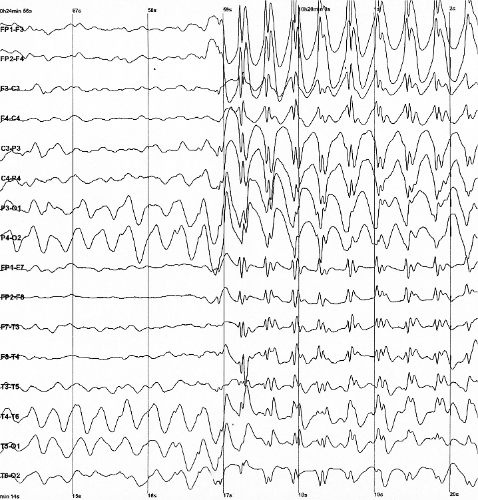
\includegraphics[width=0.6\textwidth]{eeg_example}
    \caption{Example of epileptic spikes monitored with \acs{eeg}}
    \label{fig:eeg_example}
\end{figure}

The number of electrodes used can range from a few dozen to hundreds. They are positioned on specific sections of the patient's head, therefore different electrodes monitor the activity of different areas of the brain. In this way, by looking at the \acs{eeg} and knowing the position of each electrode, the specialist can understand which areas of the patient's brain are involved in the seizure. The electrodes are identified based on whether they are placed on the left or right side of the head and also based on the lobe they are recording from (frontal lobes, temporal lobes, parietal lobes or occipital lobes). The \acs{eeg} monitoring captures several types of brain waves, which differ in the frequency. Specific ranges of frequencies are determined by particular moments of the day, situations and states of mind.

The \acs{eeg} is a very helpful tool for epilepsy diagnosis, but it cannot show for certain the presence of epileptic seizures. In fact, despite the existence of typical signal patterns associated with epilepsy, usually epileptic seizures look very different on the \acs{eeg} depending on the patient: some seizures are recognizable thanks to the presence of typical spikes in the electrical signals; other seizures happen without showing any visible change in the \acs{eeg}. Therefore, we have reason to think that for some patients the seizure is "hidden" in the relations between signals behaviour, more than in the behaviour of each signal itself. Even when the change in the \acs{eeg} pattern is clear, it could involve only a subset of electrodes (partial seizures) or all the electrodes (generalized seizures), and it is difficult to determine if the disruption of the signal is actually caused by epilepsy or if it simply represents an 'abnormal' \acs{eeg}, which could happen without the presence of seizures.

%------------------------------------------------
% Problem definition
%------------------------------------------------

\section{Problem definition} \label{sec: problem_definition}
\paragraph{} The focus of this thesis is on the problem of seizure prediction, of which we are going to analyze three different cases in order to have a clearer and more complete idea of the machine learning models potentialities on epileptic seizures data.

The seizure prediction problem can be treated as a classification problem, whose aim is to predict a class associated with each sample. In the case of an \acs{eeg}, if we consider discrete instants of time (time steps), we can represent the \acs{eeg} information as a matrix $N \times F$, where the rows represent the $N$ electrodes and the columns represent the features associated with the $F$ time steps. So, for each of the $N$ electrodes, we have a sequence of $F$ values representing the amplitude over time. The task can be treated as a classification problem by associating each time step with a label or target, which represents the class of membership between \textit{seizure} and \textit{non-seizure}. This means that each time step is classified based on the presence or absence of an ongoing epileptic seizure in that instant. If we indicate with $x_t$ the set of signals features related to a single time step, we can say that each time step $t$ with features $x_t$ has an associated target $y_t$, which is equal to $1$ if there is an ongoing seizure and to $0$ otherwise. Thus considered, the seizure prediction problem becomes the task of predicting the class target $y_t$ related to the time step's features $x_t$.

\begin{figure}[htbp]
    \centering
    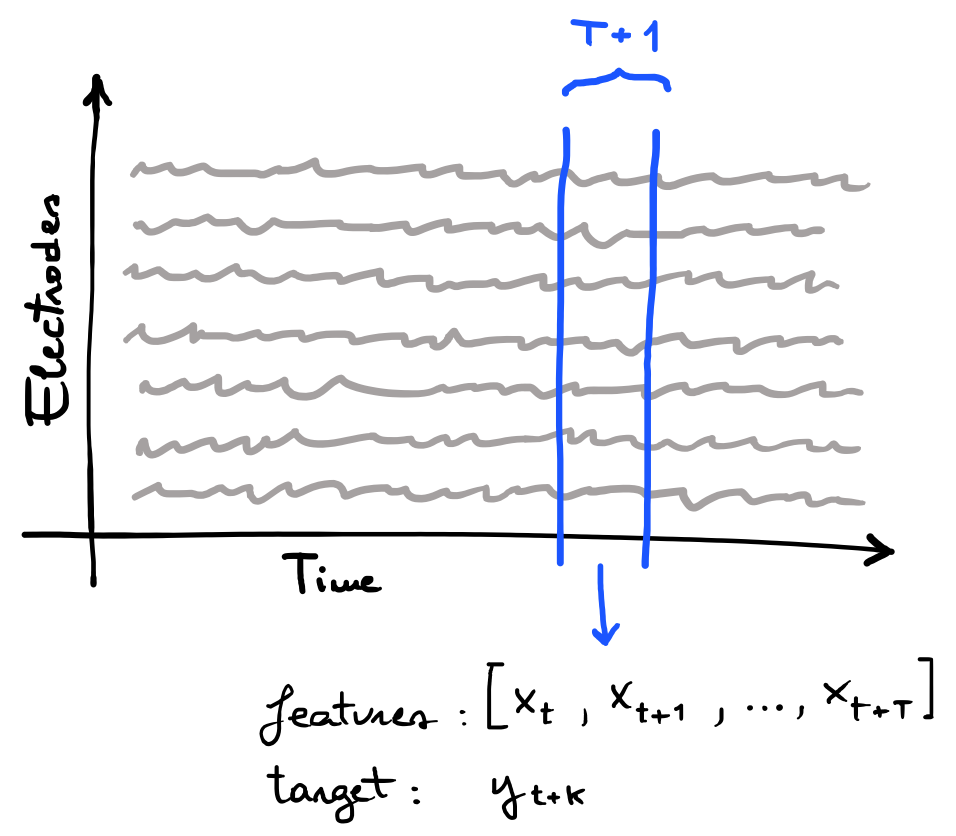
\includegraphics[width=0.6\textwidth]{problem_def}
    \caption{Problem definition}
    \label{fig:problem_def}
\end{figure}

Let's consider a time portion of $T+1$ discrete time steps in an \acs{eeg}: the portion will be characterized by a sequence of features $[x_t, x_{t+1}, x_{t+2}, ... , x_{t+T}]$, one for each time step $t$, representing the signals amplitude (measured in volts) in that instant. Let's imagine that the time portion is used to predict a single target $y_{t+k}$, which indicates whether the time step $t+k$ is part of an ongoing epileptic seizure or not. The described situation is illustrated in Figure \ref{fig:problem_def}. Considering this scenario, we can individuate three cases of study of the problem, depending on the value of the variables $T$ and $k$:
\begin{itemize}
    \item $T=0,\quad k=0$: in this case, the length of the time portion is equal to $1$ and the target corresponds to label of the single time step in the time portion (see Figure \ref{fig:problem_def1}). So at each time step $x_t$ is associated the target $y_t$ (as in the case described above). We can consider this case as a baseline scenario of the prediction problem, that is the detection based on a time step.\\
    \textsc{Example:} \quad$T=0, k=0\quad \Rightarrow{}\quad [x_3] \rightarrow{} y_3$
    \begin{figure}[h]
        \centering
        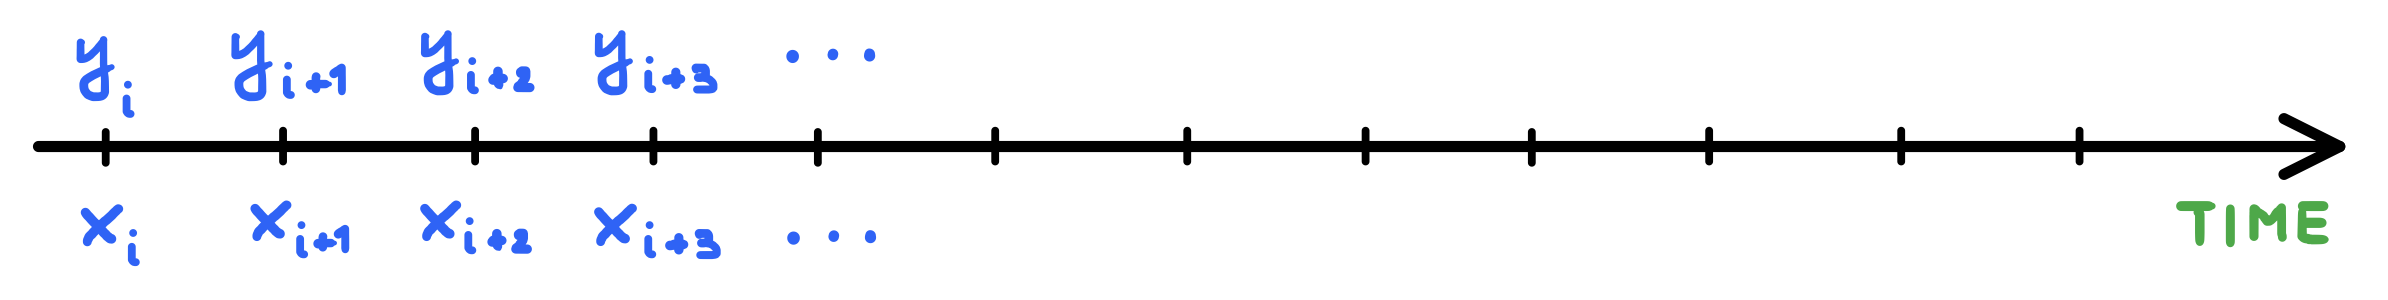
\includegraphics[width=0.8\textwidth]{problem_def1}
        \caption{Detection on a time step, representing the sample $x_i$ with target $y_i$}
        \label{fig:problem_def1}
    \end{figure}
    \item $T>0,\quad k=T$: in this case, the length of the time portion is greater that $1$, so a sample consists of a sequence of time steps, and the target is the label associated to the last time step of the sequence (see Figure \ref{fig:problem_def2}). So at each sequence $[x_t, x_{t+1}, ... , x_{t+T}]$ is associated the target $y_{t+T}$. This is still a borderline case of prediction, but with the addition of temporal dependencies between time steps, that is the detection based on a sequence of time steps.\\
    \textsc{Example:} \quad$T=5, k=5\quad \Rightarrow{}\quad [x_0, x_1, ..., x_5] \rightarrow{} y_5$
    \begin{figure}[h]
        \centering
        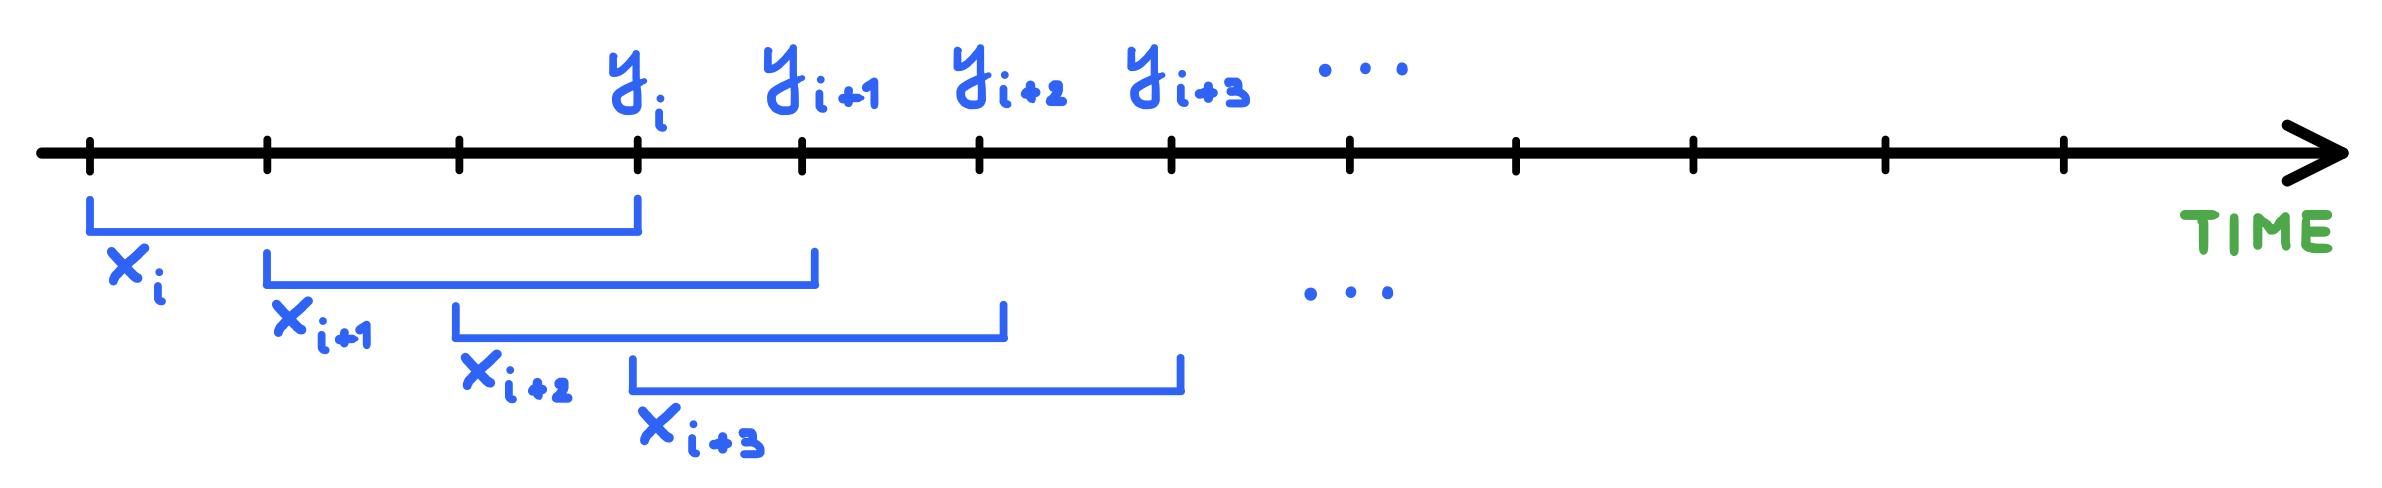
\includegraphics[width=0.8\textwidth]{problem_def2}
        \caption{Detection on a sequence, representing the sample $x_i$ with target $y_i$}
        \label{fig:problem_def2}
    \end{figure}
    \item $k>T$: in this case, we have a sequence of time steps whose target is associated to a time step that does not belong the sequence, but is forwards in time ($t>T+1$) (see Figure \ref{fig:problem_def3}). This means that at each sequence $[x_t, x_{t+1}, ... , x_{t+T}]$ is associated the target $y_{t+k}$, where $(t+k) > (t+T)$. This is the real prediction problem, since temporal dependencies are used to predict a time step some time in the future, so we are dealing with the prediction based on a sequence of time steps.\\
    \textsc{Example:} \quad$T=5, k=8\quad \Rightarrow{}\quad [x_0, x_1, ..., x_5] \rightarrow{} y_8$
    \begin{figure}[h]
        \centering
        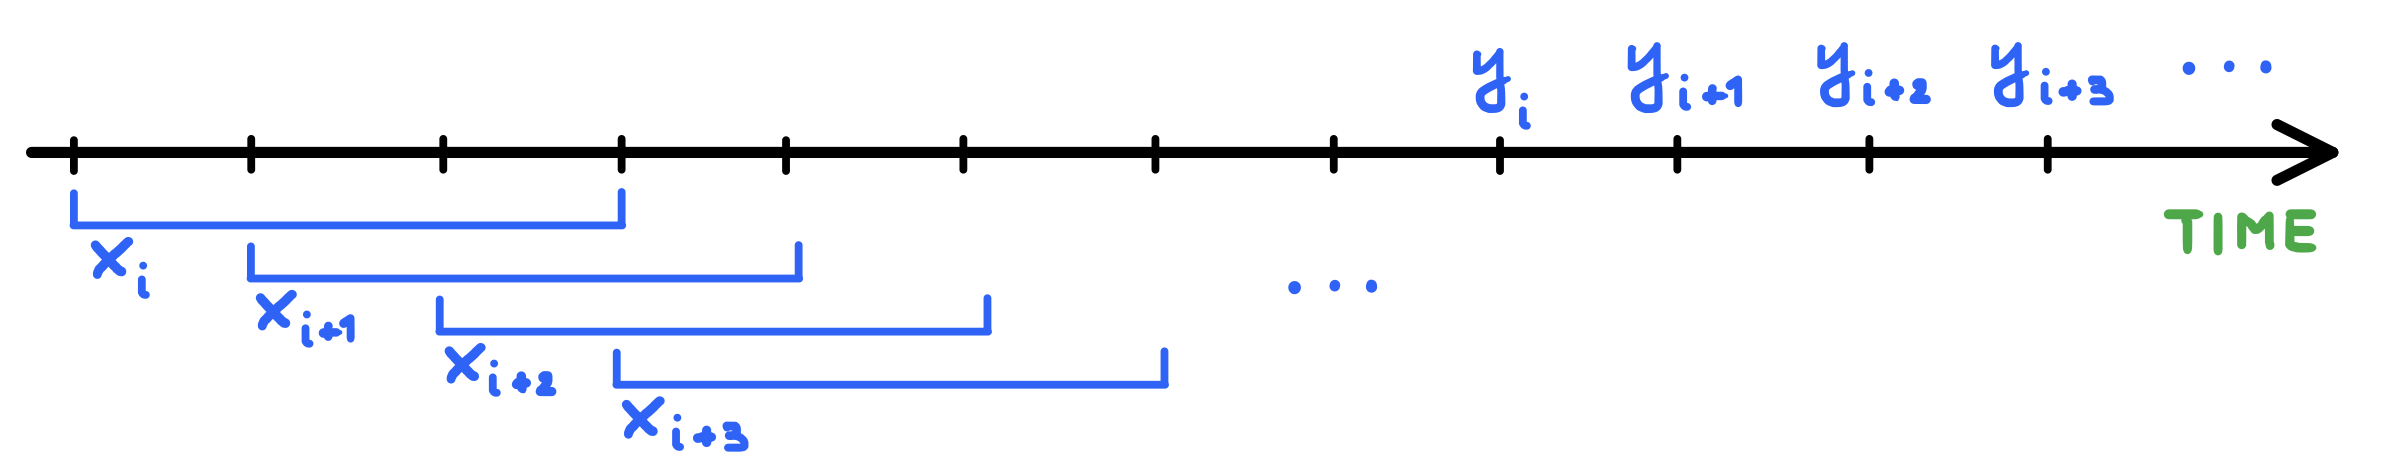
\includegraphics[width=0.8\textwidth]{problem_def3}
        \caption{Prediction on a sequence, representing the sample $x_i$ with target $y_i$}
        \label{fig:problem_def3}
    \end{figure}
\end{itemize}
The first two cases are examples of borderline cases of the prediction problem, that we define detection, since the target $y_{t+k}$ to predict is associated to a time step that is still inside the time window we look at to predict it ($k \leq T$). The third case, on the other hand, is a genuine prediction problem, since the target $y_{t+k}$ to predict is associated to a time step that is outside the time window we look at to predict it and it is forwards in time with respect to the time window ($k > T$). The difficulty of this last case is that we cannot look at the features $x_t$ in order to predict the target $y_t$, but we have to rely on information from previous time steps.

%------------------------------------------------
% Classification
%------------------------------------------------

\section{Classification} \label{sec: classification}
\paragraph{} The problem of epileptic seizure prediction can be identified as a classification task. Classification is the process of predicting the target associated with each sample in the data. In other words, the classification task consists in finding a mapping function from the input sample's features to the discrete output targets. This task is usually associated to data that can be assigned to a certain number of categories, which correspond to the targets to predict. When the data needs to be assigned to only two categories, we talk about binary classification. In this project, the problem of epileptic seizure (as described in Section \ref{sec: problem_definition}) can be considered a binary classification task, since we want to classify the time steps in two classes, which are the \textit{seizure} class and the \textit{non-seizure} class.

One of the most common methods to solve a binary classification task is logistic regression. Since the majority of models used in this project rely on logistic regression, we are going to use it as an example in order to provide a more complete description of the classification problem.

The logistic regression algorithm is used to estimate the probability that an instance belongs to a particular class \cite{OReilly:handsonML}. If the estimated probability is greater than a fixed threshold, which is commonly set to $0.5$, then the model assigns the instance to the positive class (in our case, \textit{seizure} class), otherwise it assigns the instance to the negative class (in our case, \textit{non-seizure} class). In this way, logistic regression can be used as a binary classifier.

Let's look at a very simple logistic regression model as an example: it computes the weighted sum of the input features $\mathbf{x}$ multiplied to the model parameter $\theta$ and it outputs the logistic of the result:
\begin{align}
    \hat{p} = h_{\theta}(\mathbf{X}) = \sigma\left(\theta^T \mathbf{x}\right)
\end{align}
The logistic $\sigma$ is a sigmoid function that generates a number between $0$ and $1$, representing the probability $\hat{p}$ that an instance $\mathbf{x}$ belongs to the positive class. The sigmoid function is illustrated in Figure \ref{fig:sigmoid} and it is mathematically defined as:
\begin{align}
    \sigma(t) = \frac{1}{1 + \exp{(-t)}}
\end{align}

\begin{figure}[htbp]
    \centering
    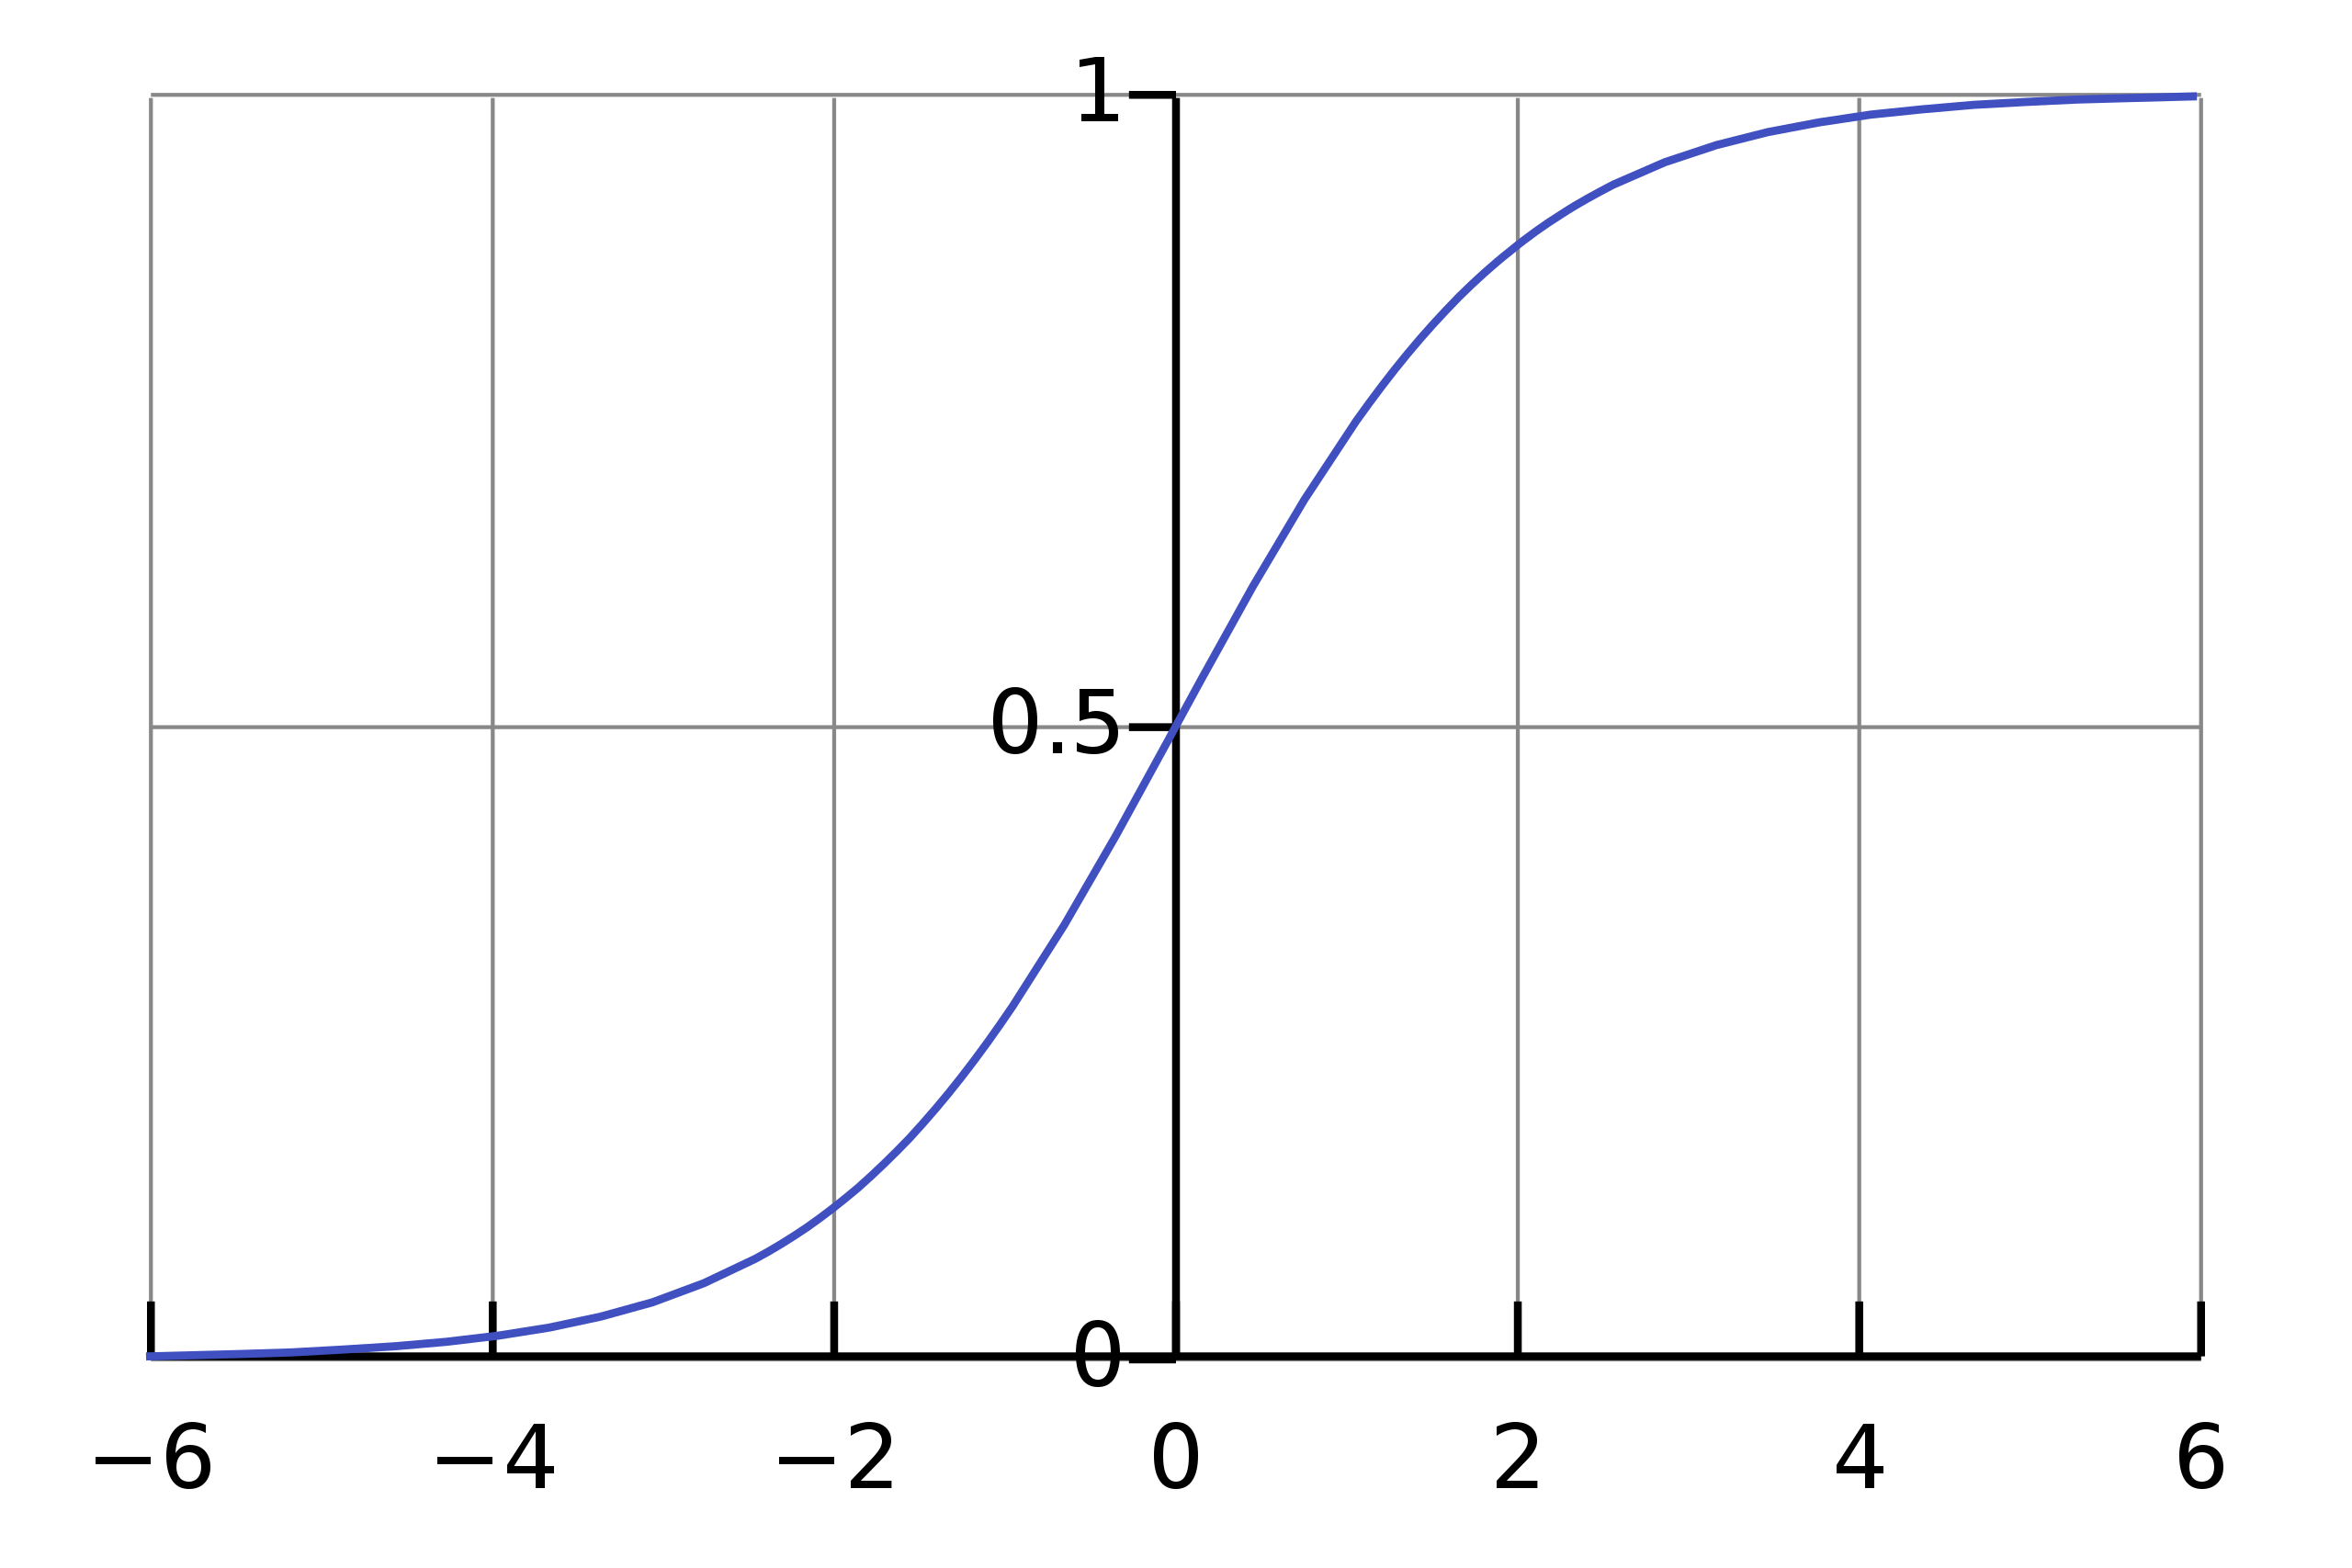
\includegraphics[width=0.6\textwidth]{sigmoid}
    \caption{Sigmoid function (from \textit{Wikipedia, the free encyclopedia})}
    \label{fig:sigmoid}
\end{figure}

The predictions $\hat{y}$ for the binary classifier can be easily obtained by applying the following equation to the estimated probability $\hat{p}$:
\begin{align}
    \hat{y} = \left\{\begin{array}{l}{0 \text { if } \hat{p}<0.5} \\ {1 \text { if } \hat{p} \geq 0.5}\end{array}\right.
\end{align}

The model parameter $\theta$ is trained in order to estimate high probabilities for positive instances and low probabilities for negative ones. In order to train it, we need a cost function that directs the model on the right track. For logistic regression algorithms, usually the most suitable cost function is the \textit{log loss}, since it captures exactly the aim of the classifier:
\begin{align}
    c(\theta) = \left\{\begin{array}{ll}{-\log (\hat{p})} & {\text { if } y=1} \\ {-\log (1-\hat{p})} & {\text { if } y=0}\end{array}\right.
\end{align}
$-\log (\hat{p})$ becomes higher and higher and tends toward infinity the more $\hat{p}$ get close to $0$, while it gets near to $0$ when $\hat{p}$ approaches $1$. $-\log (1-\hat{p})$ behaves in the opposite way, so it makes sense to use the first one for the positive class and the second one for the negative class. The cost function is applied to multiple training instances by computing the average cost over all the $n$ instances:
\begin{align}
    \textit{error } = -\frac{1}{n} \sum^{n}_{i=1}\left[y_i \log(\hat{p}_i) +
    (1 - y_i) \log(1 - \hat{p}_i)\right]
\end{align}
The log loss cost function is then used by an optimizer, for instance Gradient Descent or Root Mean Square Propagation algorithms, in order to update the model parameters accordingly. Usually, like in this project, the optimizer works on mini-batches, so the model parameters are updated after each mini-batch.

The algorithms that we studied in this work leverage this learning process, but instead of using such a simple model consisting of only one parameter, we used a set of more complex machine learning models and applied logistic regression to each of them to build several binary classifiers.

%------------------------------------------------
% Metrics
%------------------------------------------------

\section{Metrics} \label{sec: metrics}
\paragraph{} In order to evaluate the models, four metrics have been chosen, which are commonly used for binary classifiers: loss, accuracy, ROC-AUC and recall. The first two metrics are the most common performance measures for all the machine learning models.

\paragraph{Loss} The loss is the cost function evaluated on a particular set of data. In our case, we used the log loss (already described in Section \ref{sec: classification}) for deep learning models and the mean squared error (\acs{mse}) loss for classic machine learning models as cost functions. The \acs{mse} loss, also called Brier score, is the mean squared difference between the predicted probability and the actual target. The \acs{mse} loss takes values between 0 and 1 and it suggests whether the predictions are well calibrated. Its formula is:
\begin{align}
    \textit{MSE loss}=\frac{1}{n} \sum_{i=1}^{n}(\hat{p}_{i} - y_{i})^{2}
\end{align}
where $n$ is the number of samples, $\hat{p}_i$ is the predicted probability of sample $i$ and $y_i$ is the target of sample $i$.

\paragraph{Accuracy} The accuracy is simply the ratio of correct prediction, which in a binary classifier is represented by the number of true prediction (true positive and true negative) over the total number of predictions:
\begin{align}
    \textit{acc } = \frac{(TP + TN)}{(TP + TN + FP + FN)}
\end{align}
where \textit{TP} = true positive, \textit{TN} = true negative, \textit{FP} = false positive, \textit{FN} = false negative.

\paragraph{Recall} The recall, also called sensitivity or true positive rate, is the number of positive instances correctly classified over the total number of positive instances:
\begin{align}
    \textit{recall } = \frac{(TP)}{(TP + FN)}
\end{align}

\paragraph{ROC-AUC} The receiver operating characteristic curve (\acs{roc} curve) is a plot of the true positive rate (recall) against the false positive rate (shown in Figure \ref{fig:roc_auc}):
\begin{align}
    \textit{TPR } = \frac{(TP)}{(TP + FN)} \qquad\qquad \textit{FPR } = \frac{(FP)}{(FP + TN)}
\end{align}
The false positive rate is the number of negative instances incorrectly classified as positive over the total number of negative instances.
\begin{figure}[htbp]
    \centering
    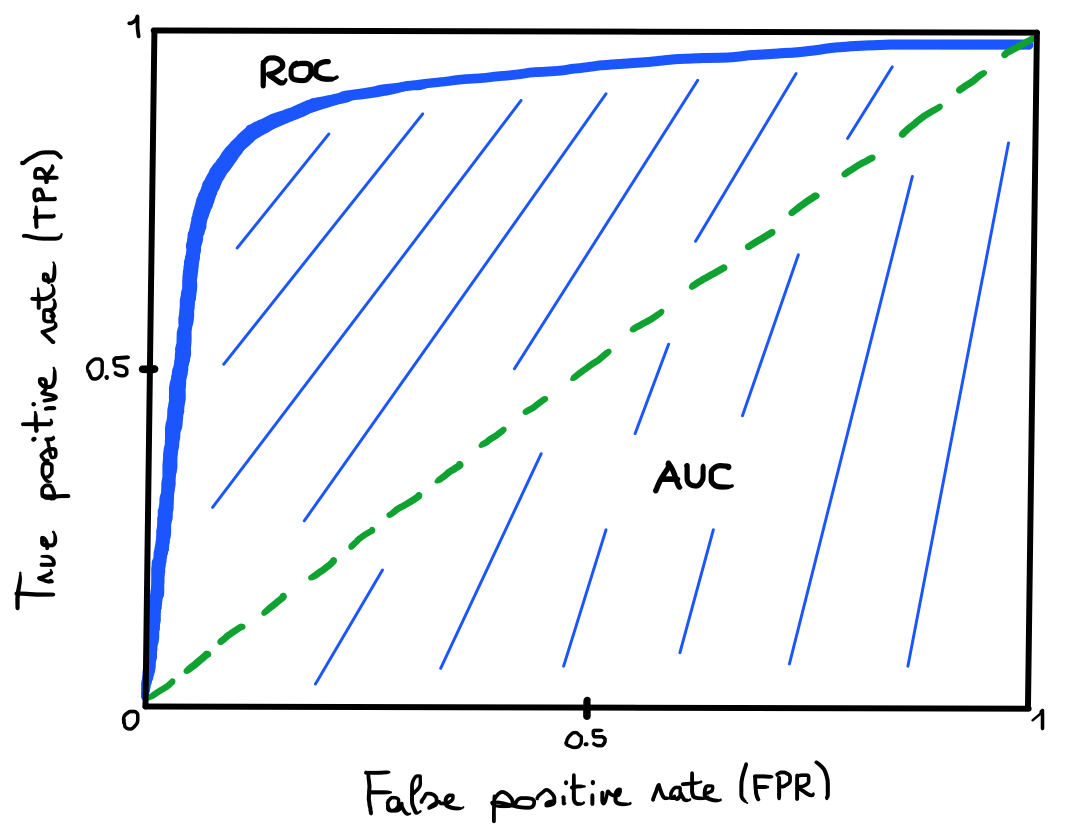
\includegraphics[width=0.6\textwidth]{roc_auc}
    \caption{\acs{roc} curve and respective \acs{auc}}
    \label{fig:roc_auc}
\end{figure}

The \acs{roc} curve represents a plot of TPR and FPR at different classification thresholds: if we lower the threshold, the classifier predicts more items as positive, so both TPR and FPR increase. In order to find the best classification threshold, we need to find a tradeoff between TPR and FPR, trying to obtain a higher TPR as possible and a lower FPR as possible (looking at the curve, we need to find the point that is closest to the upper left corner). For this purpose we can rely on the \textit{area under the \acs{roc} curve} (\acs{auc}), which provides a performance measure for different classification thresholds. The ROC-AUC ranges from 0 to 1 and its value represents the quality of the classifier predictions. A perfect classifier has \acs{auc} = 1, while a completely random classifier has \acs{auc} = 0.5.

%------------------------------------------------
% Classic machine learning models
%------------------------------------------------

\section{Classic machine learning models} \label{sec: classic_ml_models}
\paragraph{} Machine learning models are able to perform a specific task efficiently, without the need of explicit instructions, but relying uniquely on the patterns and features they learn from data. Giving the nature of this project's problem and the type of data we are working on, all the models that have been used have been trained in a supervised manner; this means that the training data fed to the algorithm includes the labels. In the case of a classification task, the training data consist of both the data features and the respective classes of membership, so that the model can learn from examples and discover patterns that allow it to make good predictions on new data.

In this section we are going to describe the classic machine learning algorithms that have been used, leaving the deep learning models (neural networks) for the next section.

\subsection{Random forest}
\paragraph{} A random forest is an ensemble of decision trees, which are machine learning algorithms able to perform both classification and regression \cite{OReilly:handsonML}. To understand how a random forest works, we first need to say a few words about decision trees.

A decision tree is a model represented as a tree in graph theory, with a root node, internal vertices, leaf nodes and edges between them. Each node can be seen as a decision unit: it contains a boolean expression based on some input features and it makes decisions based on this condition. The leaf nodes make and exception since, for classification tasks, each of them correspond to a different class. The classification of a single input instance, then, works as follows: starting from the root node, each node evaluate its boolean expression on one (or multiple) instance's feature and, depending on whether the condition is \textit{True} or \textit{False}, the path to follow continues on the left or right child of that node. The process goes on until a leaf node is reaches and the instance is finally assigned to the class corresponding to that leaf node. Figure \ref{fig:decision_tree} shows and example of a decision tree applied to the famous Iris dataset for classification. In that case, the features used by nodes to create a condition are at first the petal length and then the petal width. The three leaf nodes correspond to the tree classes: setosa, versicolor and virginica. The \textit{gini} attribute assigned to each node measures its impurity, which depends on the class distribution of the instances to which the node is applied. If $gini = 0$, then the node is pure, meaning that all the instances to which it is applied belong to the same class. If all the leaf nodes' \textit{gini} attribute is equal to zero, then the decision tree has perfectly classified all the instances.
\begin{figure}[htbp]
    \centering
    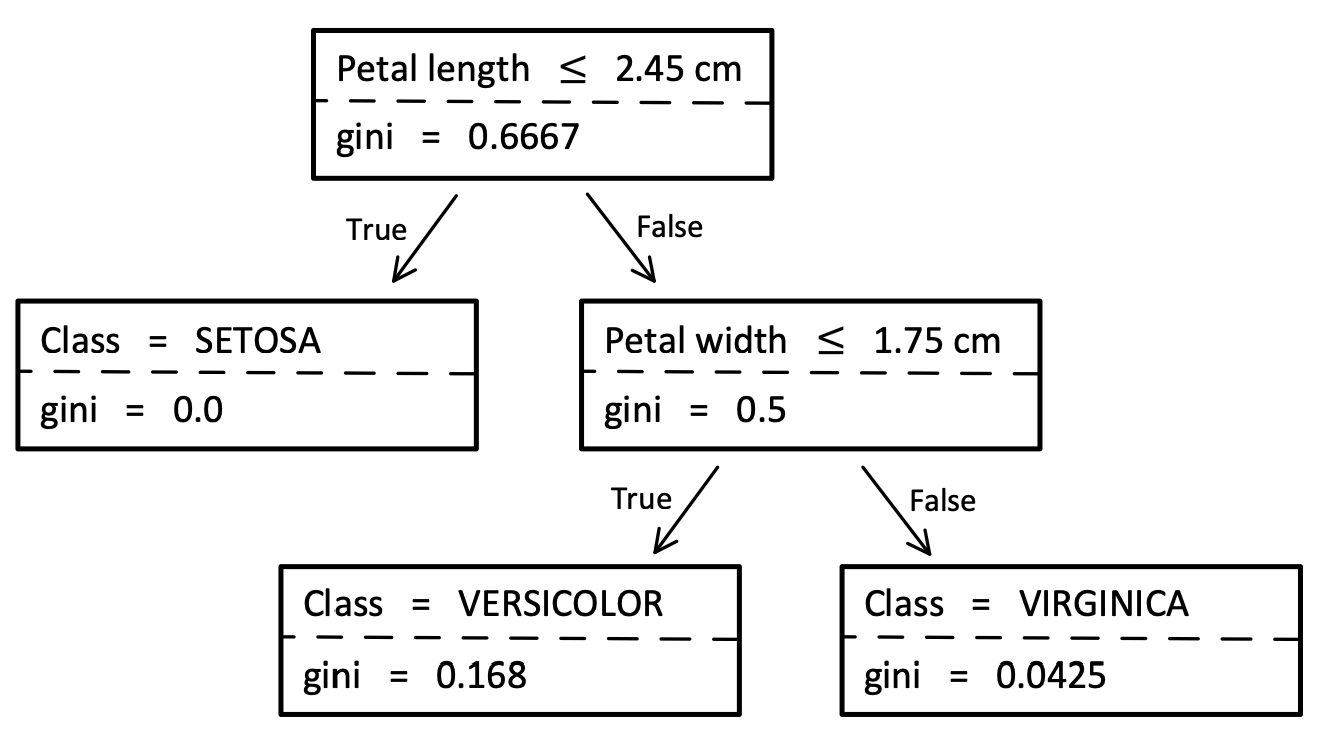
\includegraphics[width=0.7\textwidth]{decision_tree}
    \caption{Example of decision tree applied to the famous Iris dataset for classification}
    \label{fig:decision_tree}
\end{figure}

When the final prediction is computed using an ensemble of decision trees, we talk about random forest. In a random forest, $k$ different decision trees are trained in parallel on different random subsets of the training set. The sampling of the data can be performed with replacement (\textit{bootstrapping}), like in this project, or without replacement. Both methods allow training instances to be selected multiple times for different decision trees, but, when using bootstrapping, the same instance could be selected multiple times also for the same decision tree. Once all the decision trees have been trained, the random forest prediction is computed by aggregating the predictions of all its decision trees. Typically the statistical mode is used as aggregation function, but the average can be used as well. A random forest can be regularized by setting the number of decision trees to use and their maximum depth.

In general, random forest algorithms work better than decision trees and are less prone to overfitting. The reason is the greater tree diversity: in addiction to the data sampling, when splitting a node during the construction of the tree, the split is chosen no longer as the best among all features, but as the best among a random subset of the features.

\subsection{Gradient boosting}
\paragraph{} Gradient boosting (tree-based) is very similar to random forest, as it is itself an ensemble of decision trees. Differently from random forest, in gradient boosting the decision trees are trained in a sequential way, one at a time, and each one tries to correct the errors made by its predecessor. In particular, each new decision tree is fitted on the residual errors made by the previous one. Therefore, while the first decision tree of the sequence will fit the instances $\mathbf{X}$ and the targets $\mathbf{y}$, the second decision tree will fit $\mathbf{X}$ and the residual errors $y_1 = \mathbf{y} - \hat{y}_1$, where $\hat{y}_1$ are the predictions made by the first decision tree on $\mathbf{X}$. Likewise, the third decision tree will fit $\mathbf{X}$ and the residual errors $y_2 = y_1 - \hat{y}_2$, where $\hat{y}_2$ are the predictions made by the second decision tree on $\mathbf{X}$, and so on. So we can consider gradient boosting as a gradient descent algorithm.

Usually gradient boosting have better performance with respect to random forest, but, since decision trees are not trained independently, it is more prone to overfitting.

\subsection{Support vector machine}
\paragraph{} \acf{svm} is a very powerful machine learning algorithm able to perform both linear and non-linear classification and regression \cite{OReilly:handsonML}. It is a binary classifier, but it can be used also as a multiple-class classifier. In order to classify data, the \acs{svm} represents the instances as points on a decision surface and divides them through a decision boundary that is placed in the middle of the largest possible gap between the two classes' instances (positive and negative class). In other words, if we imagine the data projected in a 2-dimensional space, the \acs{svm} tries to find a line able to separate the positive and negative instances staying as far away as possible from the closest instances. This situation is illustrated in Figure \ref{fig:svm_line}, where the two group of instances, belonging to the blue and green classes, are divided by the red line. The boundary generated by the \acs{svm} is placed as far as possible from the instances, trying to maximize the distance $w$ from the nearest instances. In this way, in case we made a small error in the location of the boundary, we have a margin of error that prevents a misclassification. The instances that lie on the edges of the decision boundary's margins are called \textit{support vectors} (in Figure \ref{fig:svm_line} they are represented as filled circles). The position of the support vectors completely determines the max-margin decision boundary and the distance between support vectors of different classes determine the width of the optimal boundary’s margins.
\begin{figure}[htbp]
    \centering
    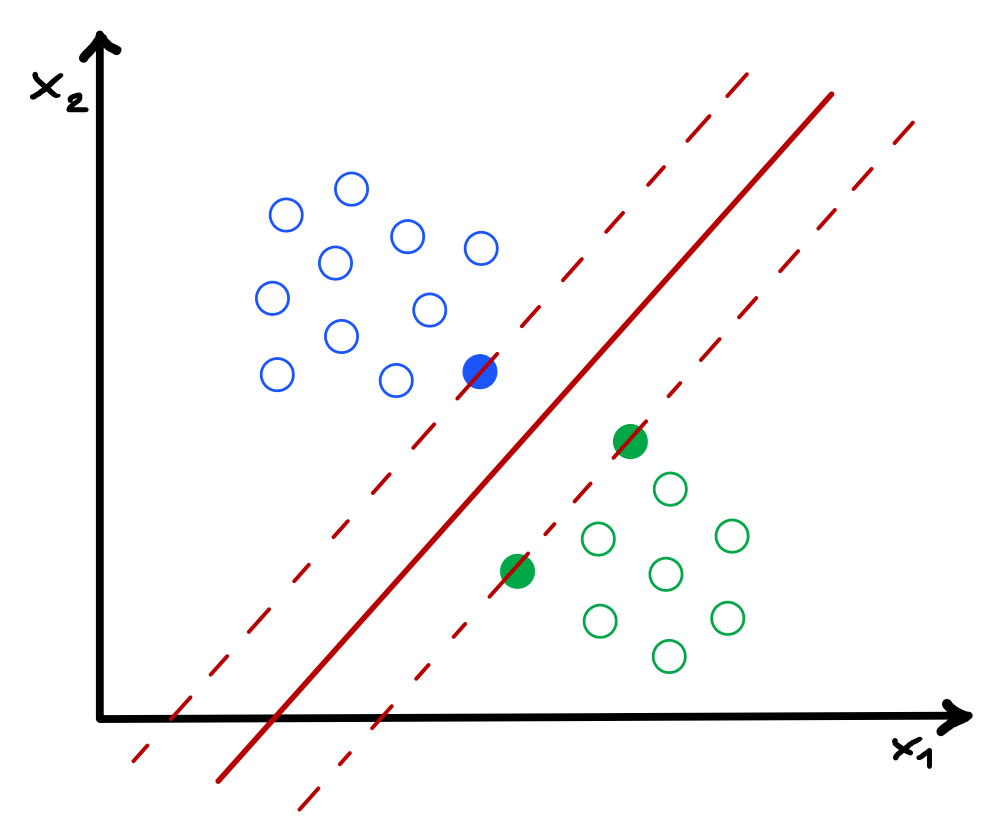
\includegraphics[width=0.4\textwidth]{svm_line}
    \caption{Example of \acs{svm} decision boundary for data classification}
    \label{fig:svm_line}
\end{figure}

In the general case with $d$-dimensional data, \acsp{svm} find a ($d-1$)-dimensional hyperplane such that the margin of separation between the two classes is maximized.

If the data points are linearly separable, the \acs{svm} is able to construct two parallel hyperplanes that separate the data points in the two respective classes. The hyperplanes can be respectively described by the two equations:
\begin{align}
    &\vec{w} \cdot \vec{x}^{+}-b=1 \\
    &\vec{w} \cdot \vec{x}^{-}-b=-1
\end{align}
The distance between the two hyperplane is $\frac{2}{\|\vec{w}\|}$, so, in order to maximize the distance between them, we want to minimize $\|\vec{w}\|$, while avoiding margin violations (\textit{hard margin}) or limiting them (\textit{soft margin}).

Hard margin can be used for problems where the data points are linearly separable. In this case, the max-margin hyperplane is completely determined by those data points which are nearest to it and we want to prevent data points from falling into the margin. To reach this result, we can use the following objective function, subjected to the following constraints:
\begin{align}
    &\text{objective function }= \min \frac{1}{2}\|\vec{w}\|^2 =  \min \frac{1}{2} w^{T} w\\
    &\text{constraints }= \left\{\begin{array}{ll}{\text{if } y=1 :} & {w^{T} x+b \geq 1} \\ {\text{if } y=0 :} & {w^{T} x+b <-1}\end{array}\right.
\end{align}
These constraints guarantee that each point lies on the correct side of the margin.

In some cases, the problem can be non-linear and therefore not solvable with hard-margin; in other cases, the problem can be linear, but we would like a general solution that takes into account the presence of some errors in the data. In these situations, soft-margin can be used in place of hard-margin. Soft-margin \acsp{svm} allow some exceptional data points to fall into the margin or to lie on the wrong side of the margin. Soft-margin \acs{svm} introduces two new parameters: $\varepsilon_i$ represents the distance of $x_i$ from his true class margin hyperplane; $C$ is a parameter that allows to control better the softness of the margin, defining the tradeoff between the objective and the constraints. If $C$ is very big, the \acs{svm} becomes very rigid and behaves similarly to hard-margin; on the other hand, if $C$ is very small, the \acs{svm} imposes a smaller penalization for misclassified samples. Soft-margin is defined by the following objective function, subjected to the following constraints:
\begin{align}
    &\text{objective function }= \min \frac{1}{2} w^{T} w + C \sum^{n}_{i=1} \varepsilon_i\\
    &\text{constraints }= \left\{\begin{array}{lll}{\text{if } y=1 :} & {w^{T} x+b \geq (1 - \varepsilon_i)} \\ {\text{if } y=0 :} & {w^{T} x+b < (-1 + \varepsilon_i)} \\ {\text{for all } i :} & {\varepsilon_i \geq 0}\end{array}\right.
\end{align}
Figure \ref{fig:svm_formulas} shows a geometric representation of the parameters and formulas just presented.
\begin{figure}[htbp]
    \centering
    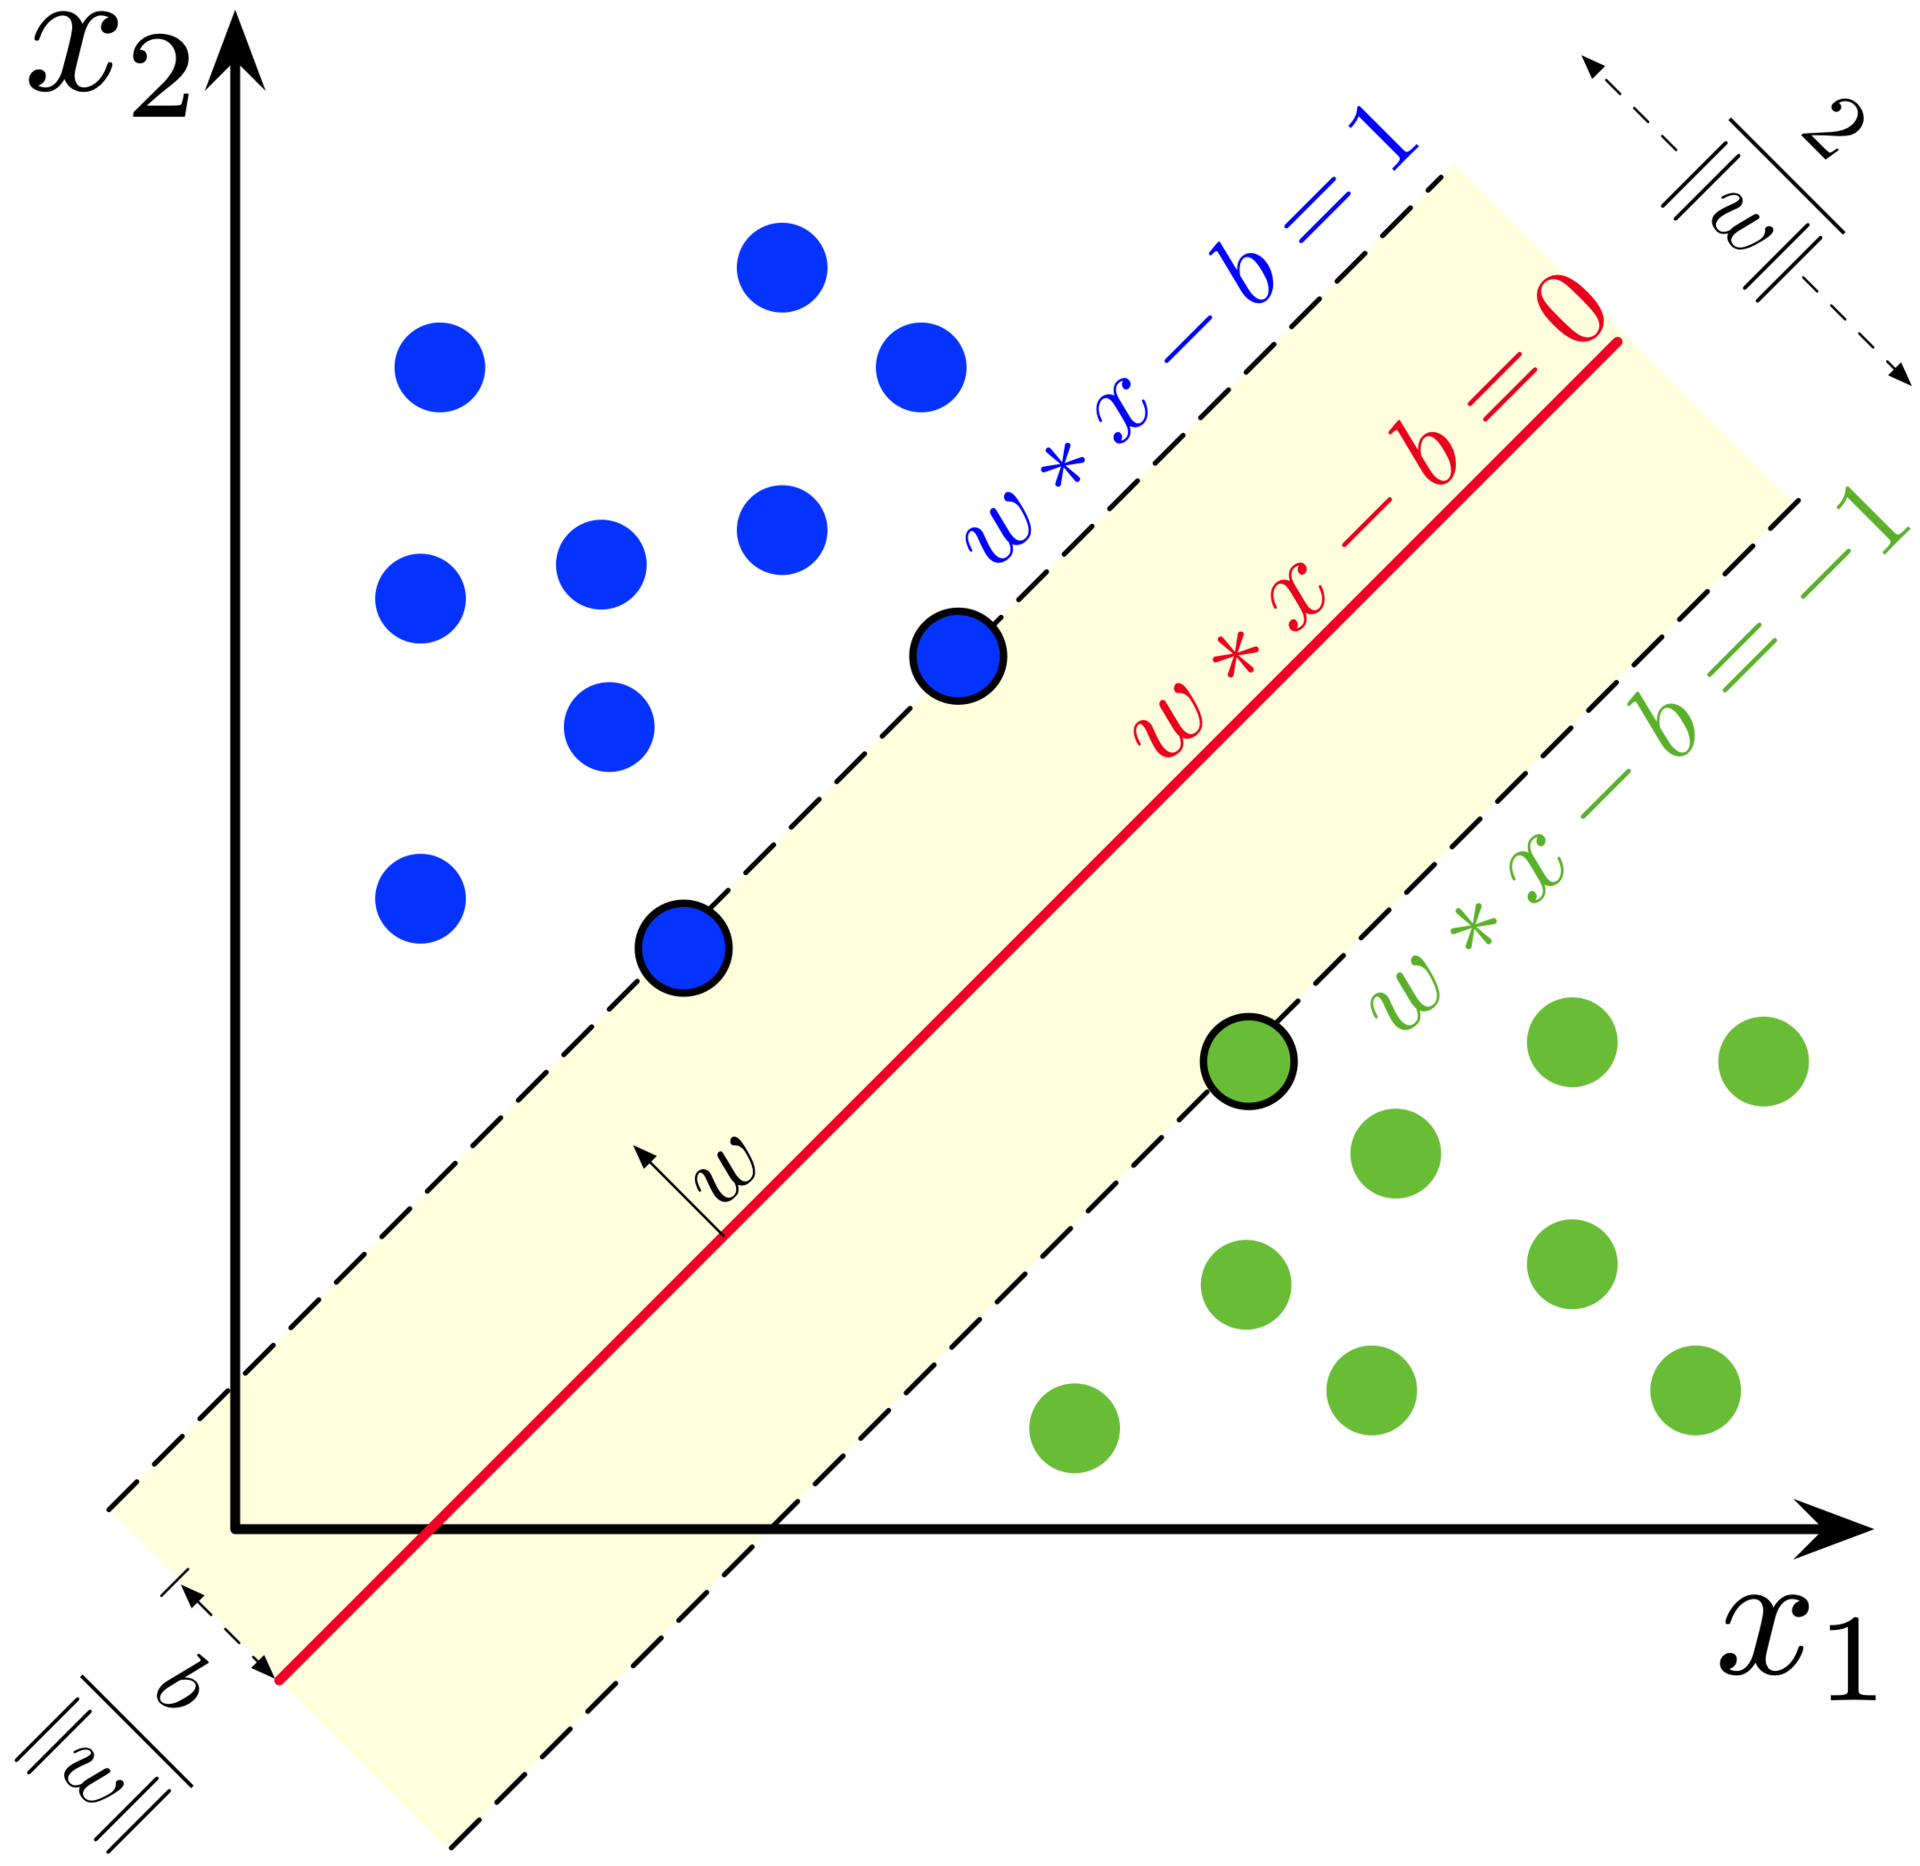
\includegraphics[width=0.4\textwidth]{svm_formulas}
    \caption{Geometric representation of \acs{svm}'s equations}
    \label{fig:svm_formulas}
\end{figure}

When data are not linearly separable, we can still use \acs{svm} in two ways: we can simply use soft-margin and permit some tolerance in presence of errors, or we can rely on a kernel function $K(a, b)$. A kernel function allows the \acs{svm} to lead the data points to a situation where they are linearly separable again. Indeed, the data can be mapped to a higher-dimensional feature space, where they are linearly separable by an optimal hyperplane. A feature map is the function that maps the data points to an higher-dimensional feature space: the function $\phi(x_i)$ maps every $x_i$ to the new feature space:
\begin{align}
    <\phi(a), \phi(b)>
\end{align}
The increase of space's dimensions can be computationally expensive, due to the computation of all the additional features. To avoid an high-cost computation, we can use the \textit{kernel trick}: applying a kernel function allows to compute the dot product of weights in the lower-dimensional space instead of in the higher-dimensional space:
\begin{align}
    <\phi(a), \phi(b)> = K(a, b)
\end{align}
The trick consists in expressing the problem just in function of the dot products, without the need to know the entire mapping to the new feature space. Actually, a kernel is a function that is able to compute the dot product $\phi(a)^T \phi(b)$ based only on the original vectors $a$ and $b$, without the need to compute the transformation $\phi$ on the vectors. Figure \ref{fig:svm_nonlinear} shows an example of a non-linear separable problem that could be solved by mapping data to a higher-dimensional space.
\begin{figure}[htbp]
    \centering
    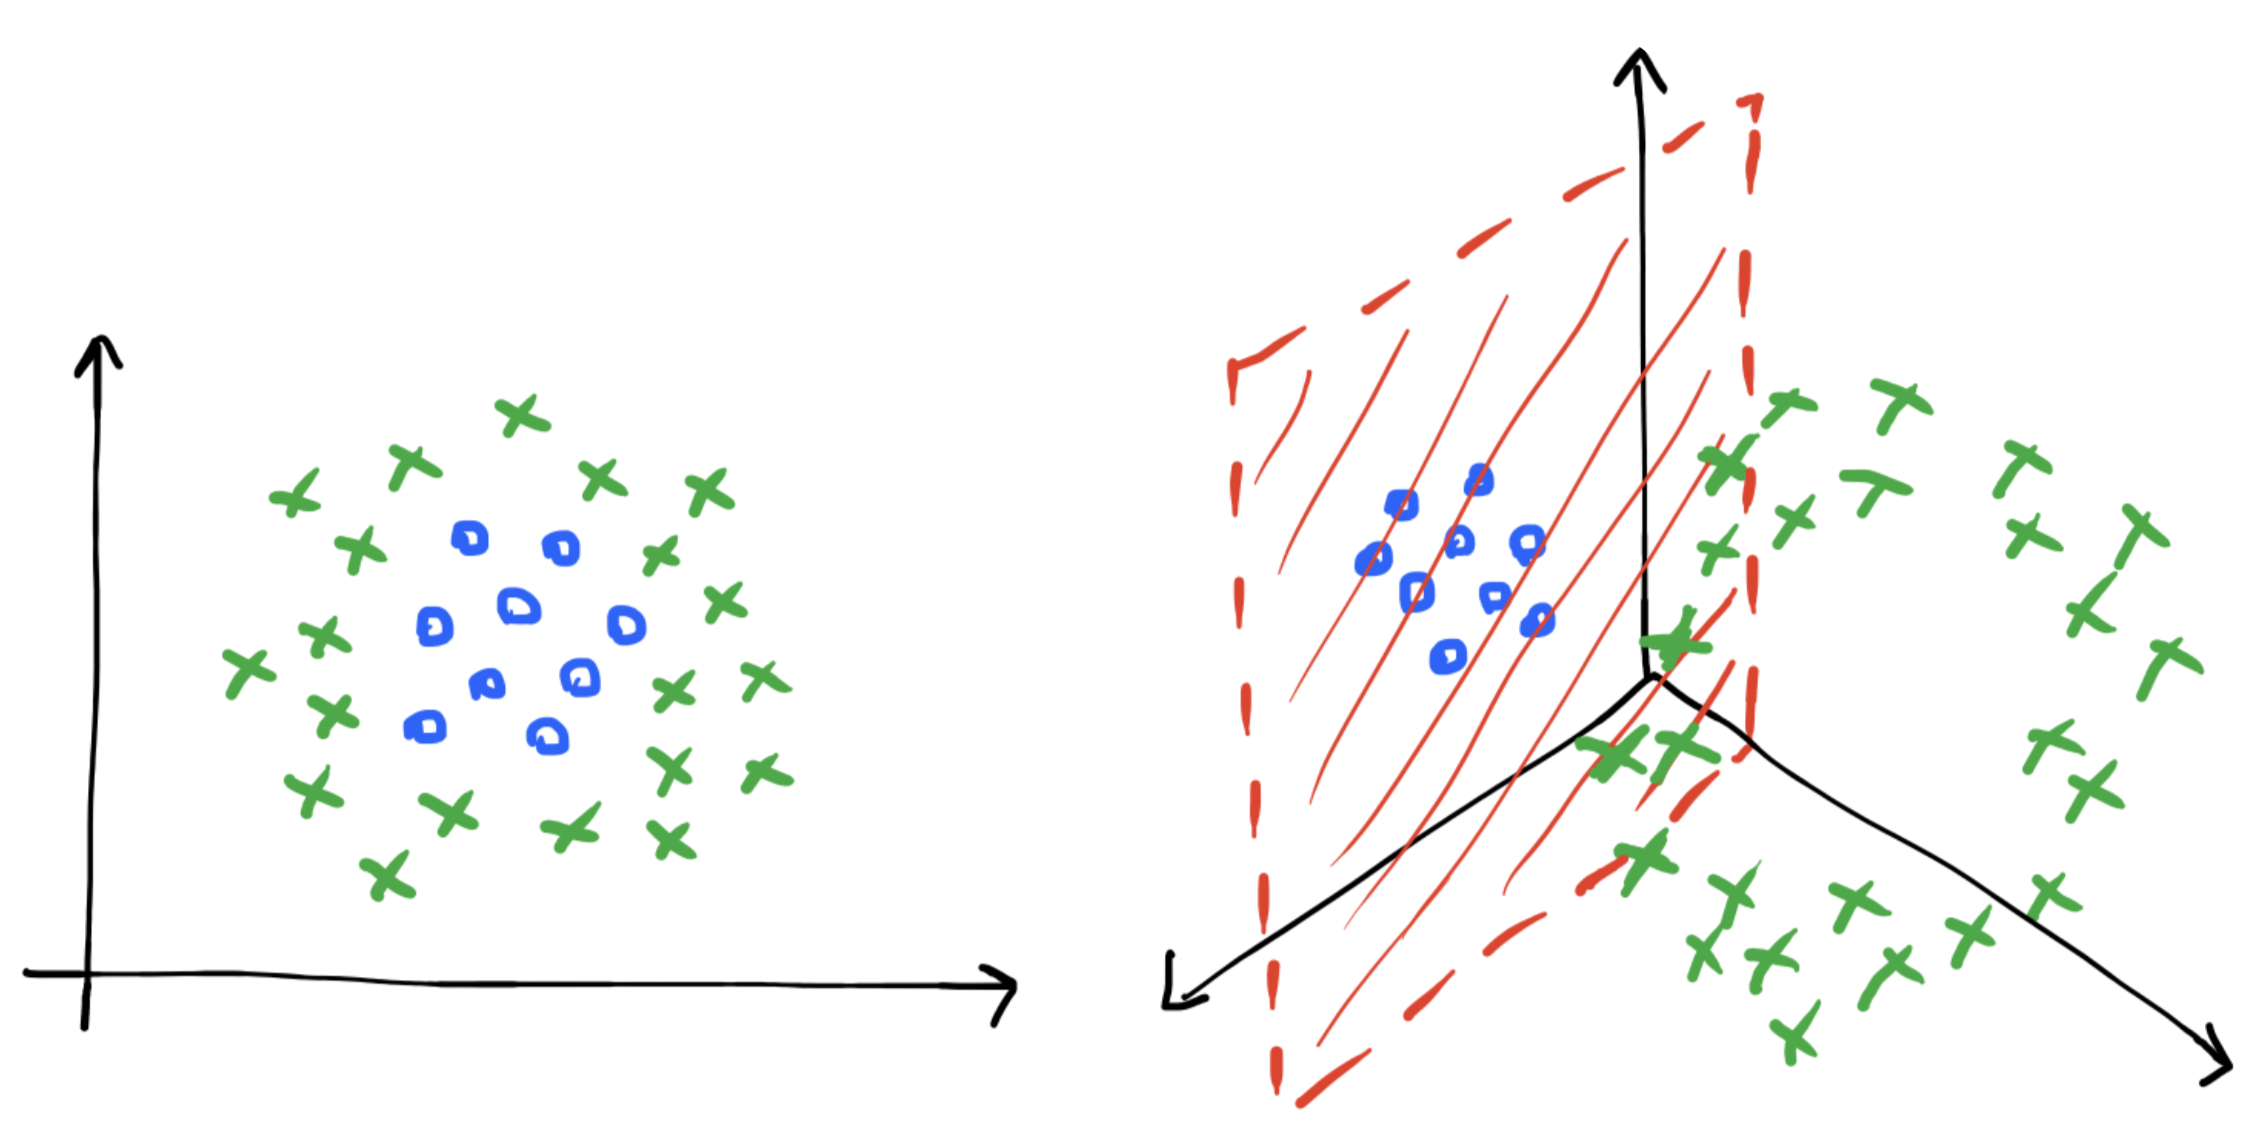
\includegraphics[width=0.6\textwidth]{svm_nonlinear}
    \caption{Example of a non-linear separable problem solved in a higher-dimensional space}
    \label{fig:svm_nonlinear}
\end{figure}

A frequently used kernel is the Gaussian \acf{rbf} kernel. This kernel generates new features by measuring the distance between the support vectors and all other instances: the function value decreases as the distance from the support vectors grows, so it can be considered a similarity measure. Through Gaussian \acs{rbf} kernel, the input vector is mapped to an infinite vector and then normalized by dividing each component by the vector’s length. The Gaussian \acs{rbf} kernel is defined by the equation:
\begin{align}
    K(a, b) = \exp \left(-\frac{\|a - b\|^{2}}{2 \sigma^{2}}\right) = \exp \left( -\gamma \|a - b\|^{2} \right)
\end{align}
The hyperparameter $\gamma = \frac{1}{2 \sigma^{2}}$ can be used as regularization term, since it controls how strict the decision boundary is by determining a strong sharpness if $\gamma$ is big (if $\sigma$ is small) and a weak sharpness otherwise (if $\sigma$ is big). So if the \acs{svm} is overfitting, $\gamma$ should be reduced, and if it is underfitting, $\gamma$ should be increased.

The kernel trick can be used together with the soft-margin in order to reach good performance and better generalization.

%------------------------------------------------
% Deep learning models
%------------------------------------------------

\section{Deep learning models} \label{sec: dl_models}
\paragraph{} Deep learning is a subfield of machine learning that differentiate itself for the specific type of models that it uses in order to learn a certain task. Deep learning models use a hierarchical representation of the features in order to make predictions \cite{Nvidia:dl}. Like other machine learning algorithms, deep learning models automatically extract common patterns found in the data, which become the crucial features to be used in the classification or regression process. The difference with standard machine learning methods is in the way the features are gathered. Deep learning models organize the feature identification in a hierarchical way, by extracting multiple layers of non-linear features to be used for making predictions. The \textit{deep} hierarchy of non-linear features allows the model to learn more complex features with respect to standard machine learning algorithms. The most common deep learning models, which make use of a hierarchical representation of the features, are \textit{artificial neural networks}.


\subsection{Artificial neural networks}
\paragraph{} Artificial neural networks, or simply neural networks (\acsp{nn}), are very powerful and versatile models that are inspired by human neural networks: the structure of artificial neural networks is comparable to the one of our brain, which has neurons and connection between them to transmit electrical impulses. Similarly, artificial neural networks are composed by several neurons which are the computational cores of the model and which transmit the processed information to each other.

Neural networks organize the neurons in layers: the input layer is represented by the input data, the output layer is the last one that process data and returns the result of the entire model, while all the layers in between are called \textit{hidden layers} and, in addition to transforming the data, they send the processed information to the next layer. Figure \ref{fig:nn_layers} shows an example of a typical network's structure.
\begin{figure}[htbp]
    \centering
    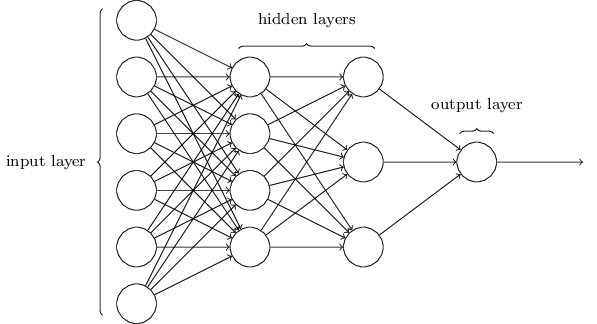
\includegraphics[width=0.7\textwidth]{nn_layers}
    \caption{Neural network's structure and layers (from \textit{Neural Networks and Deep Learning} free online book)}
    \label{fig:nn_layers}
\end{figure}

The most classic form of neural networks is the \textit{feed-forward neural network} \acs{fcnn}, also called dense neural network. A \acs{fcnn} consists of a sequence of fully-connected layers \cite{OReilly:TFforDL}. Each layer represents a function (linear and non-linear transformations) from $\mathbb{R}^F$ to $\mathbb{R}^{F_m}$. This means that, for each input instance having $F$ features, the corresponding output will have dimensionality $F_m$, where $F_m$ is the number of neurons in the network's output layer (the $m$-th layer). Even for the hidden layers, the output dimension depends on the number of neurons present in the layer.

The network is called \textit{fully-connected} because the output of each neuron in one layer is sent as input of each neuron in the next layer, so there is a direct connection between all the neurons belonging to subsequent layers. Figure \ref{fig:nn_dense} shows and example of dense neural network, making visible the full interconnection between subsequent layers.
\begin{figure}[htbp]
    \centering
    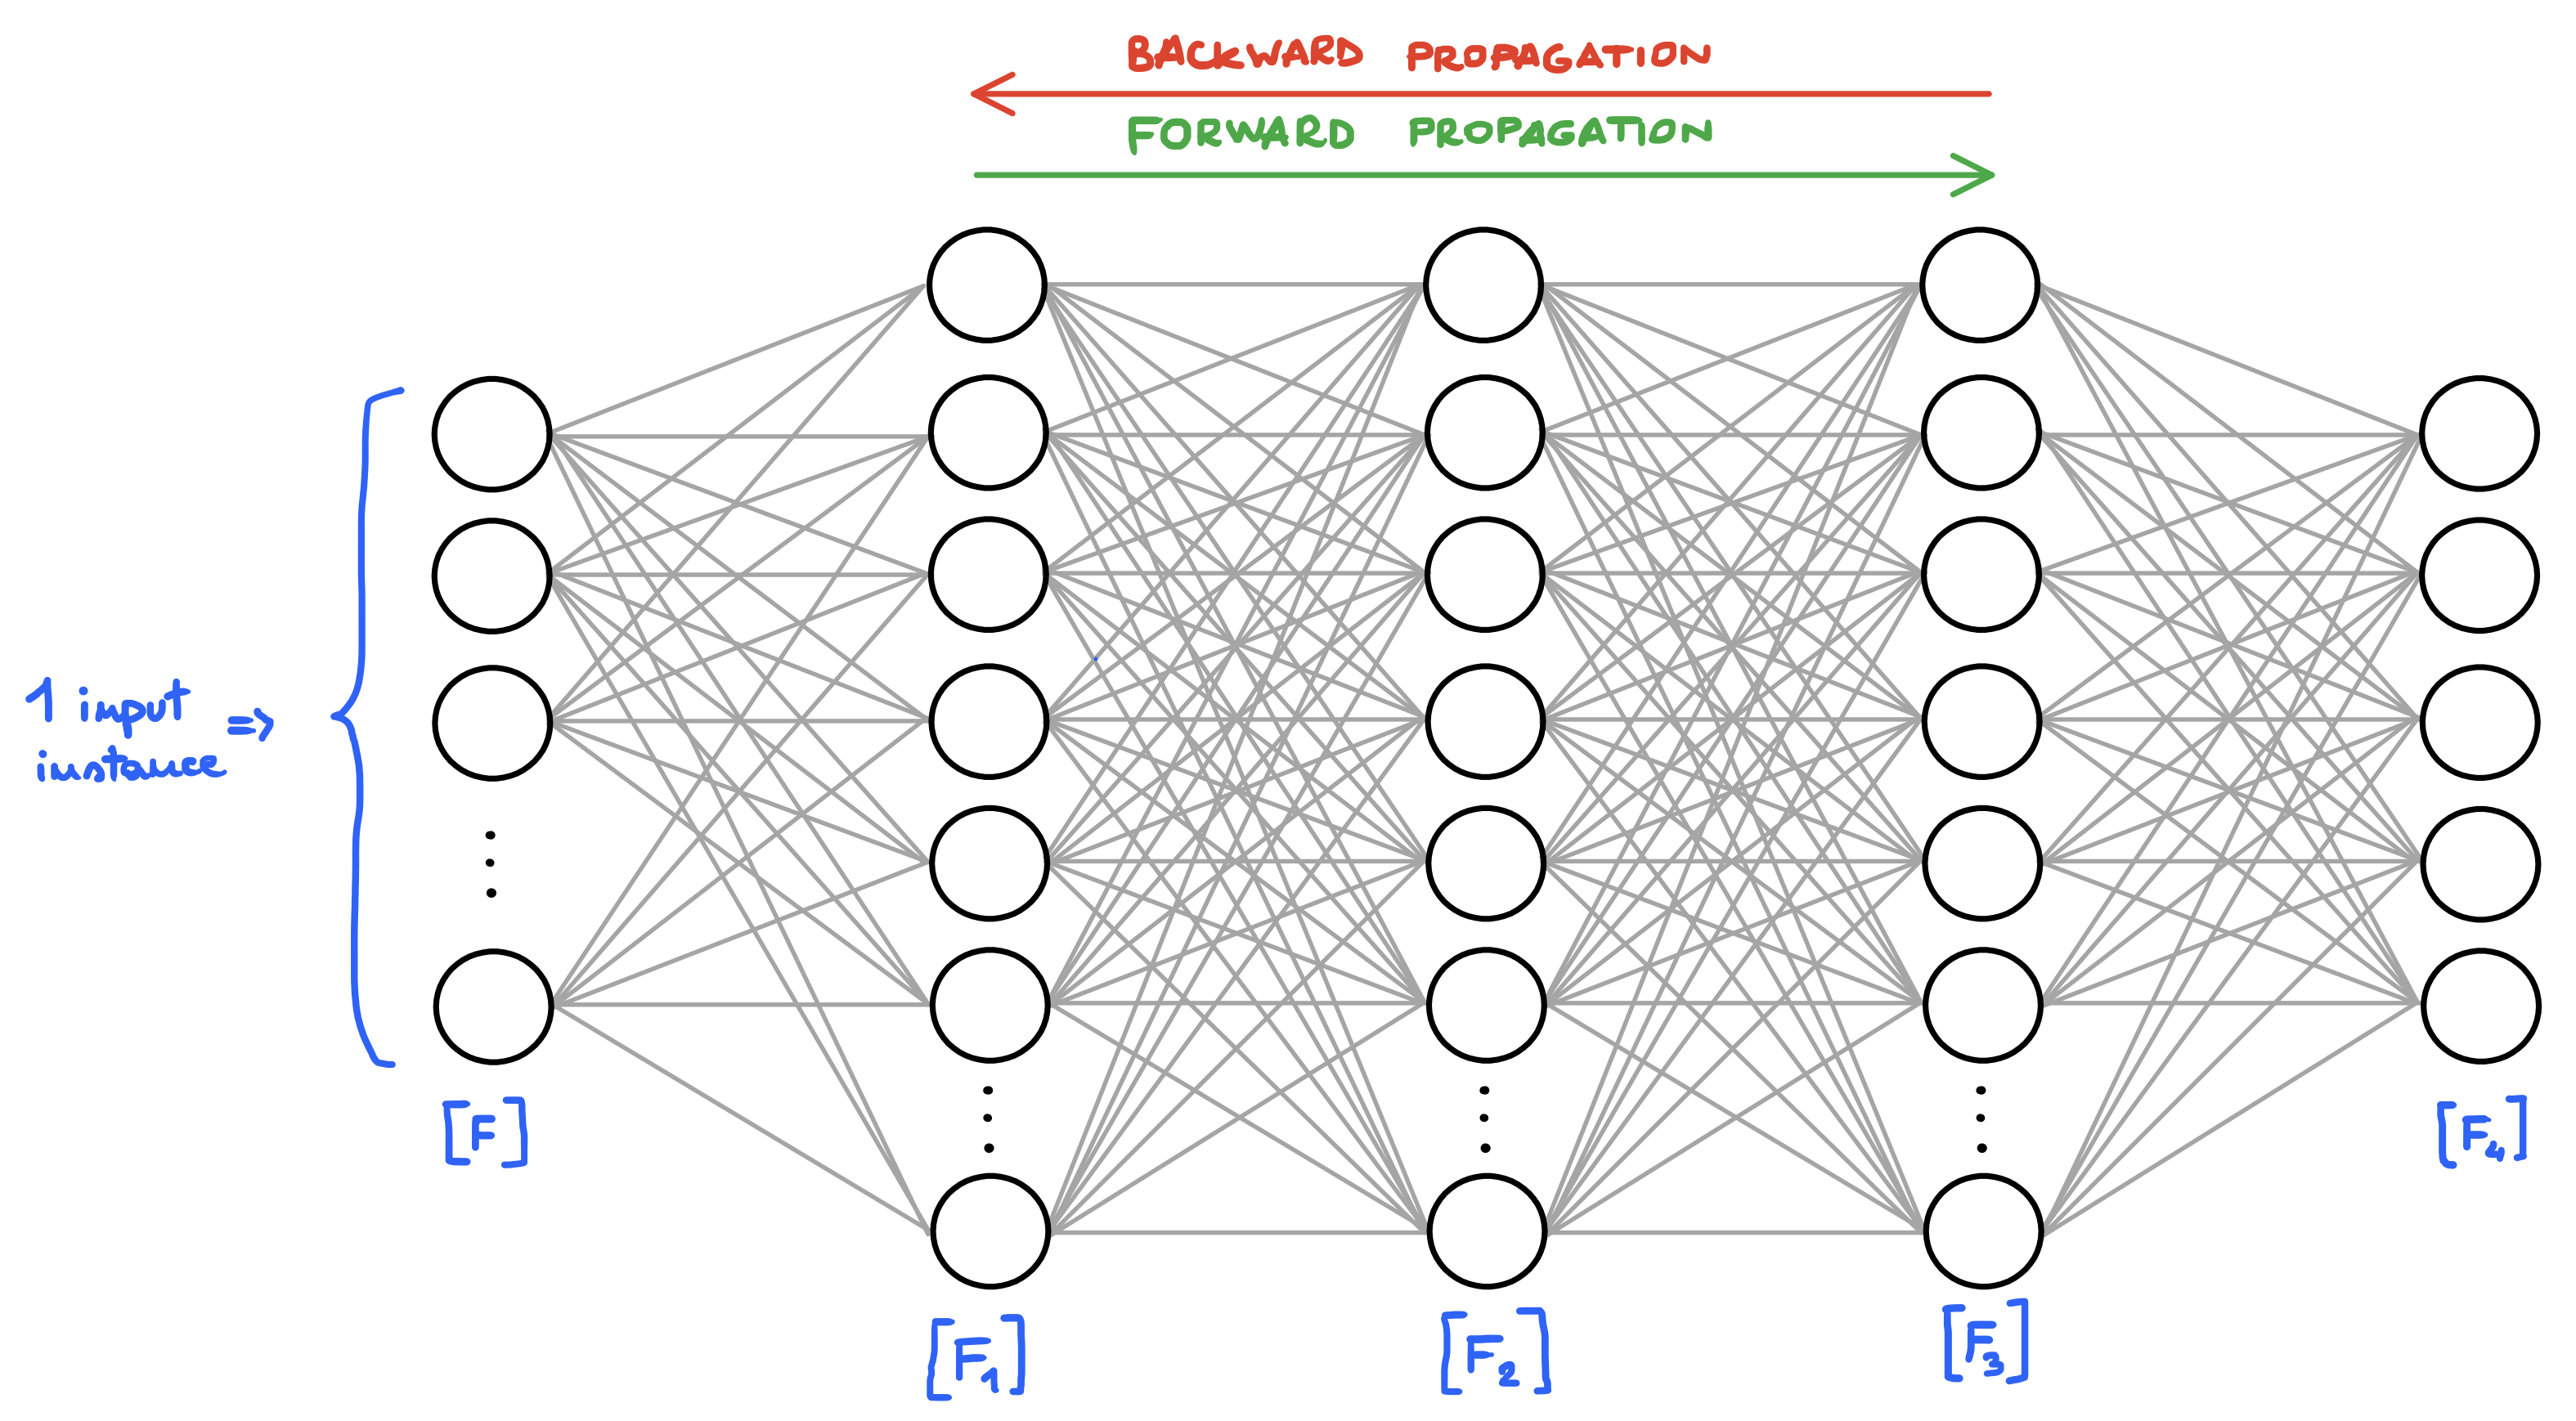
\includegraphics[width=0.9\textwidth]{nn_dense}
    \caption{Example of dense neural network}
    \label{fig:nn_dense}
\end{figure}

Each neuron processes the input data by computing the following transformation:
\begin{align}
    \mathbf{x}_{i}^{l}=\sigma\left(\sum_{j} \mathbf{w}_{ij}^{l} \mathbf{x}_{j}^{l-1} + \mathbf{b}_{i}^{l}\right)
\end{align}
where the subscript represent the $i^{th}$ or $j^{th}$ neuron of the layer in the superscript, which is the $l^{th}$ or $(l-1)^{th}$ layer, $\mathbf{x}$ represents the input features, $\mathbf{w}$ represents the correspondent weights, $\mathbf{b}$ represents the bias term, usually equal to 1, and $\sigma$ represents the activation function. The weighted sum plus the bias term form the linear part of the transformation, followed by the non-linear part, which is the application of the activation function. The bias term helps the network approximating the objective function; while the activation function, as already mentioned, introduces the non-linearity properties by mapping the data to the desired output. Figure \ref{fig:nn_neuron} illustrates the functioning of a single neuron.
\begin{figure}[htbp]
    \centering
    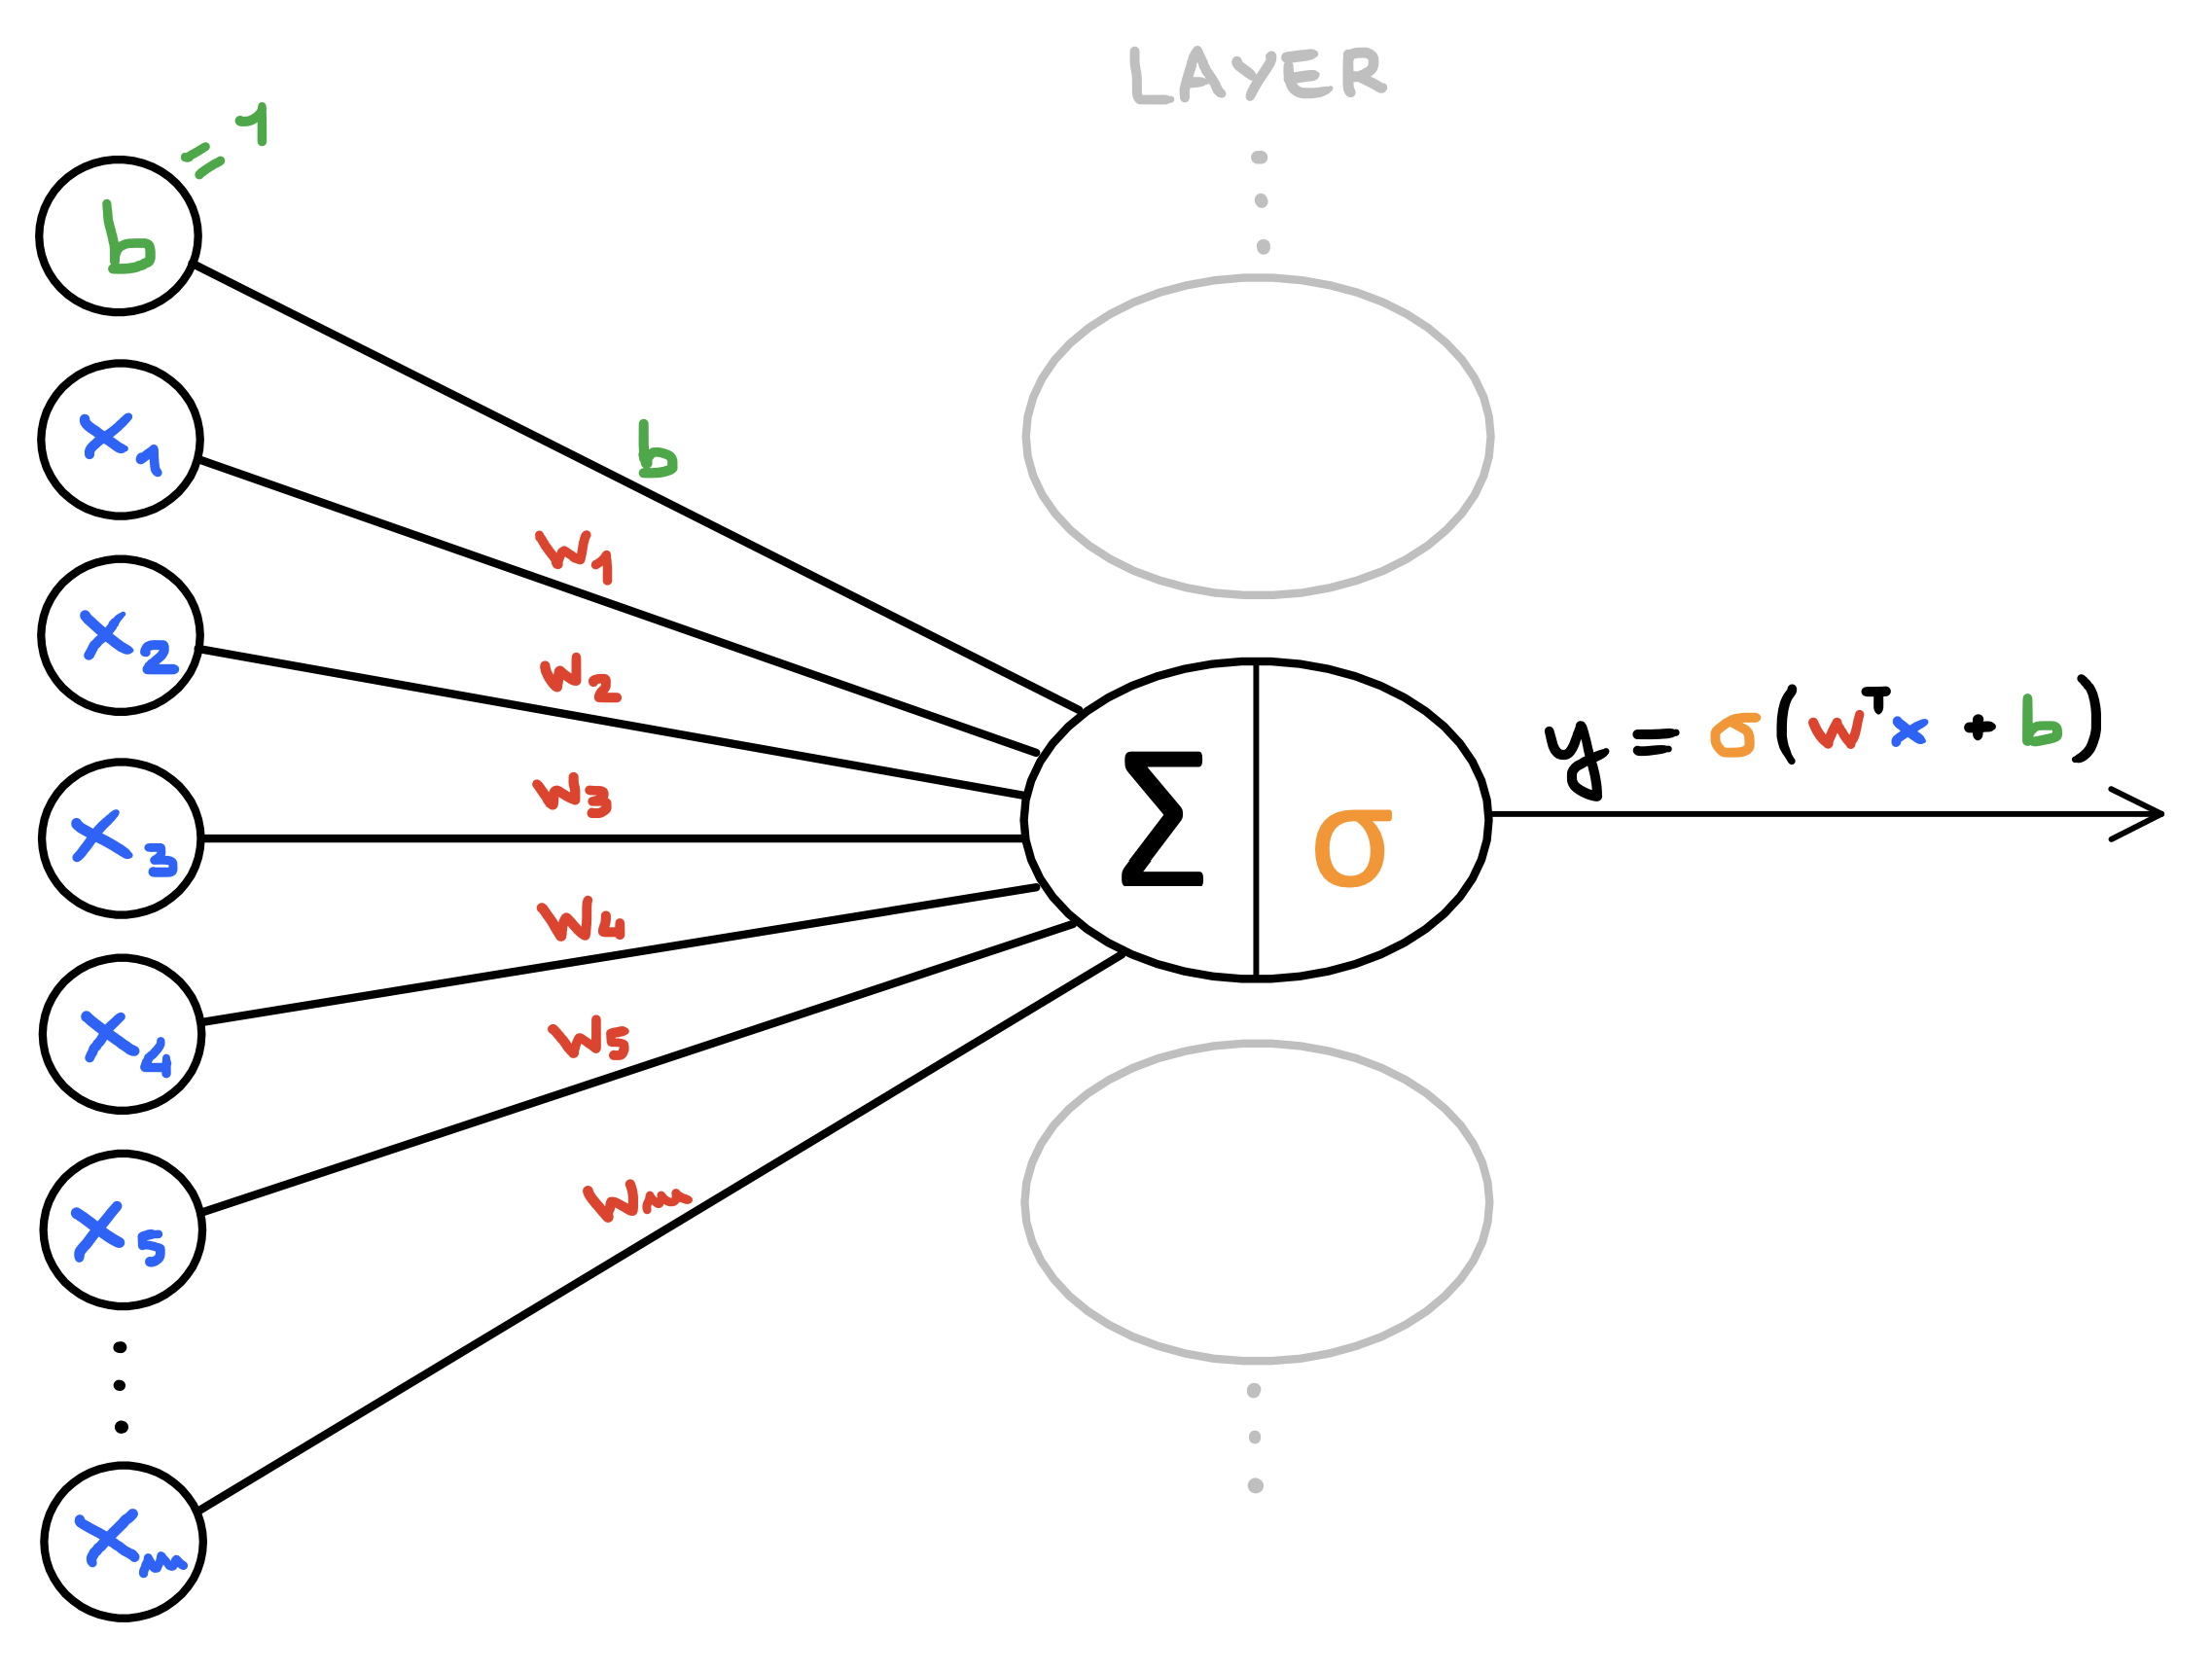
\includegraphics[width=0.6\textwidth]{nn_neuron}
    \caption{Illustrated description of the functioning of a single neuron}
    \label{fig:nn_neuron}
\end{figure}

Each neuron in a layer performs this operation and the outputs of all the neurons of that layer will be the inputs for the next layer. Formally, the inputs and outputs of layers of a neural network can be described by the equations:
\begin{align}
    &h^{\textit{out}}_{0} = \mathbf{X}\qquad\qquad\qquad \text{(input layer)}\\
    &h^{\textit{in}}_{i} = h^{\textit{out}}_{i-1} \times \mathbf{W}_i + \mathbf{B}_i\\
    &h^{\textit{out}}_{i} = \phi_i (h^{\textit{in}}_{i})
\end{align}
where $\mathbf{X}$ is the features matrix of input data, $\mathbf{W}_i$ is the weights matrix of layer $i$, $\mathbf{B}_i$ is the bias vector of layer $i$, $\phi_i$ is the activation function used by neurons of layer $i$, and the operator $\times$ represents matrix multiplication.

When used for classification tasks, the output layer of a \acs{fcnn} has a number of neurons that is equal to the number of classes of the data. In this way, each output of the network (computed through softmax or sigmoid activation function) corresponds to the estimated probability that the input instance belongs to the corresponding class. The instance is then assigned to the class which obtained higher probability.

\subsection{Neural network's training process}
\paragraph{} The training process of neural networks takes places through two steps: the forward and backward propagations. For each training input instance, the model computes the output of every neuron in each consecutive layer until it reaches the final predictions from the output layer (\textit{forward pass)}. After that, it compares its prediction with the actual targets and measures the output error. The error is then propagated through each layer in reverse in order to compute the error contribution (error gradient) from each neuron's connection, until it reaches the input layer (\textit{backward pass}). The error is then used by the optimizer to update the connections weights and allow the model to learn. The neural networks in which the activation flows only in one direction are included in the category of feed-forward neural networks.

The \textit{backpropagation} represents the core of the learning process of a neural network, since it is the procedure to update the model's learnable parameters. After the generation of the predictions (forward pass), the gradient of the loss function with respect to the weights is computed; then the weights are updated in the opposite direction of the gradient. This operation is called \textit{Gradient Descent}. The "magnitude" of the update is given by the \textit{learning rate}, which can be decisive in the search for the loss function's global minimum.


\subsection{Optimizers}
\paragraph{} An optimization algorithm determines the way in which the model's parameters (\textit{weights}) are updated during the training process. The aim of an optimizer is to minimize an objective function that is dependent on the model's weights, which is the cost function. Since the cost function is computed using the model's predictions and the latter are determined by the weights and input features, the weights have a crucial role in minimizing the cost function. Since the weights values are determined by the Gradient Descent, the role of an optimizer is to optimize the Gradient Descent process, in order to make it more efficient and effective. In this project, the optimizer that has been used for all the models is the \acf{adam} optimizer.

\paragraph{\acs{adam} optimizer} \acs{adam} is one of the most popular and used optimizers in deep learning, that usually has good performances. It is based on two intuitions: adaptive learning rate (inspired by RMSProp optimizer) and momentum optimization \cite{arXiv:adam} \cite{arXiv:optimizers}. An adaptive learning rate method computes individual learning rates for different model's learnable parameters; while a momentum method helps accelerating the Gradient Descent process by adding a fraction of the update vector of the past time step to the current update vector. This optimizer stores two moments: the first moment $m_t$ (the mean), which is estimated as the exponentially decaying average of past gradients, and the second moment $v_t$ (the uncentered variance), which is estimated as the exponentially decaying average of past squared gradients. The two moments are computed respectively as follows:
\begin{align}
    m_{t} &=\beta_{1} m_{t-1}+\left(1-\beta_{1}\right) g_{t} \\
    v_{t} &=\beta_{2} v_{t-1}+\left(1-\beta_{2}\right) g_{t}^{2}
\end{align}
where $g_{t}$ is the gradient on current mini-batch and $\beta_1$, $\beta_2$ are optimizer's decay rates, usually set close to 1. Since $m_t$ and $v_t$ are initialized as zero-vectors, they are biased towards zero, therefore they need to be corrected:
\begin{align}
    \hat{m}_{t} =\frac{m_{t}}{1-\beta_{1}^{t}} \qquad\qquad\qquad
    \hat{v}_{t} =\frac{v_{t}}{1-\beta_{2}^{t}}
\end{align}
The first moment $m_t$ is used as momentum optimization parameter, while the second moment $v_t$ is used to adapt the learning rate to each different weight. The resulting \acs{adam} update rule for model's weights is the formula:
\begin{align}
    \theta_{t+1}=\theta_{t}-\frac{\eta}{\sqrt{\hat{v}_{t}}+\epsilon} \hat{m}_{t}
\end{align}
where $\theta$ is the model weight and $\eta$ is the learning rate ($\epsilon$ is just a smoothing term usually initialized to a tiny number).


\subsection{Activation functions}
An activation function is a non-linear mapping between the input and the output. Activation functions are essential in neural networks layers, since they introduce the non-linearity properties to the model: without activation functions, the neural network would be a simple linear transformation and it would not be able to learn from complex data.

Some activation functions are more suited to hidden layers, while others are perfect to compute the final output of the model. In this project, we used the sigmoid function as activation function for the last layer of our models in order to classify data, as previously explained in Section \ref{sec: classification}. For the hidden layers, we used both \acf{relu} and \acf{tanh} activation functions.

\paragraph{ReLU} \acs{relu} is a very popular and extremely fast and effective activation function for hidden layers. Its principle is very simple: it keeps only positive values, while setting to 0 all the negative ones.
\begin{align}
    \text{R}(x) = max(0, x)
\end{align}
The \acs{relu} function is illustrated in Figure \ref{fig:relu}. The \acs{relu} activation function is very effective for very deep networks, since it helps avoiding the vanishing gradient problem. This problem arises when the gradient of the loss function, used to update the model's weights, assumes too small values during the backpropagation across the layers and the network is not able to learn anymore. \acs{relu}, thanks to the sparsity of its outputs, helps avoiding this problem.

\paragraph{Tanh} \acs{tanh} is similar to sigmoid, but it ranges from $-1$ to $1$. It maps negative input as strongly negative, positive ones as strongly positive and zero inputs near zero. Its formula is:
\begin{align}
    \tanh{(x)} = \frac{e^{2x} - 1}{e^{2x} + 1}
\end{align}
The \acs{tanh} function is illustrated in Figure \ref{fig:tanh}.
\begin{figure}[htbp]
    \centering
    \begin{subfigure}[t]{0.5\textwidth}
		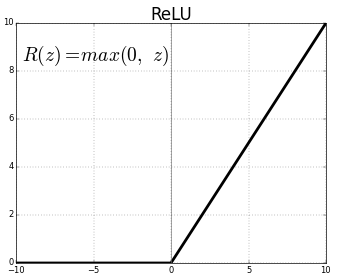
\includegraphics[width=0.9\textwidth]{relu}
        \caption{ReLU activation function (from \textit{Medium})}
        \label{fig:relu}
	\end{subfigure}%
	~
	\begin{subfigure}[t]{0.5\textwidth}
		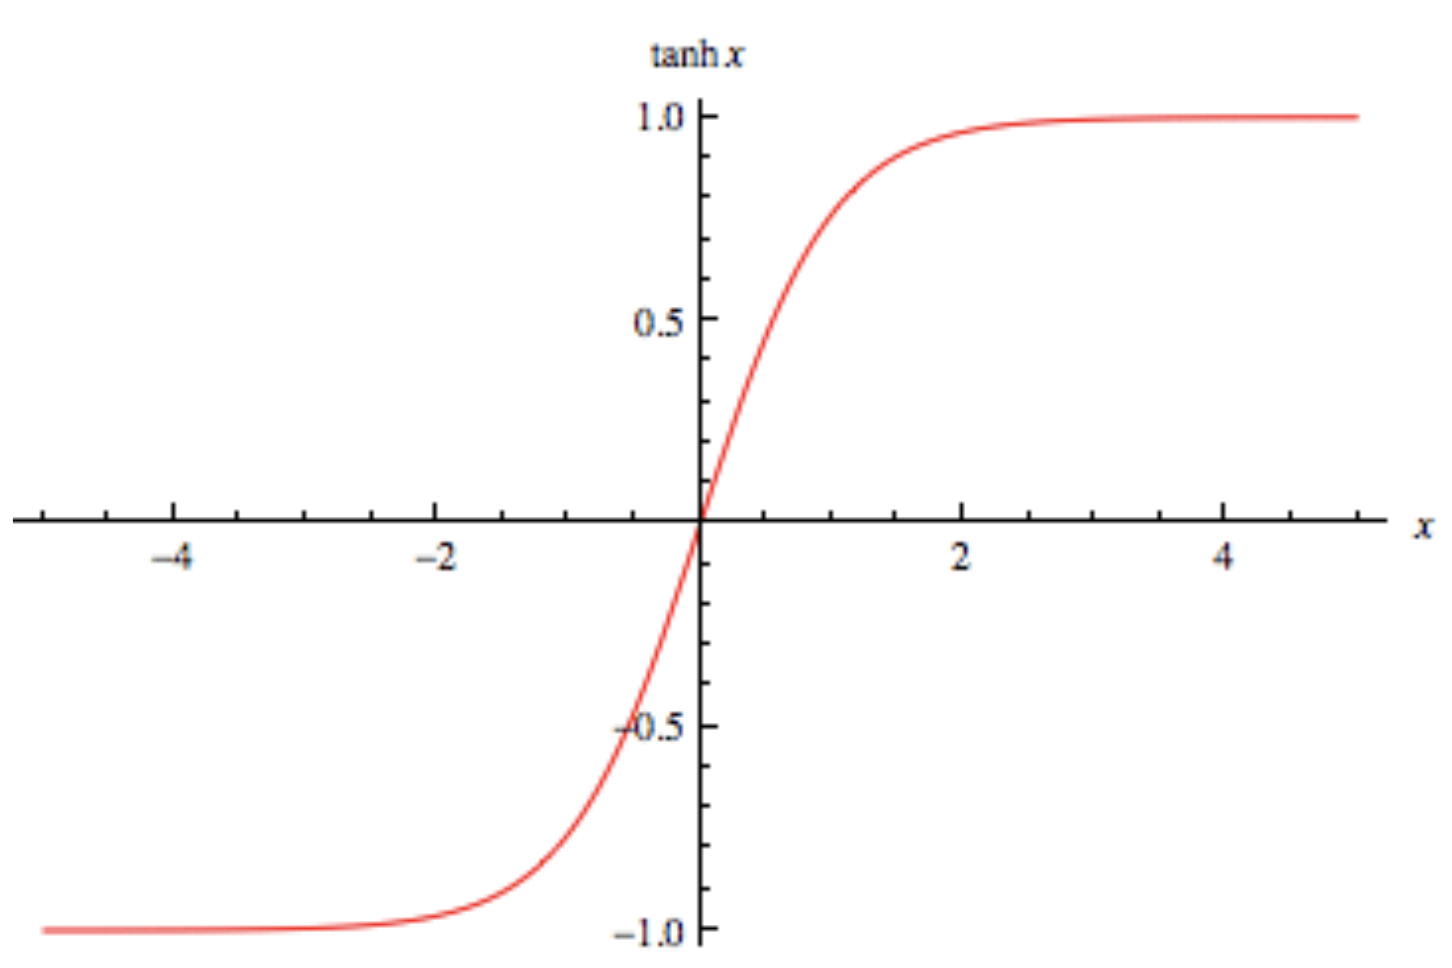
\includegraphics[width=1\textwidth]{tanh}
        \caption{Tanh activation function (from \textit{Wolfram MathWorld})}
        \label{fig:tanh}
	\end{subfigure}
	\caption{Activation functions}
\end{figure}


\subsection{Regularization}
\paragraph{} Regularization techniques are very useful in deep learning in order to avoid overfitting. Deep neural networks generally have a huge amount of parameters, which represent their power to learn from complex datasets; this flexibility, however, sometimes leads to the overfitting of the training set, preventing the model from making good predictions on any other dataset \cite{OReilly:handsonML}. To solve this problem, there exist several regularization methods, which in some way limit the amount of freedom of the model by encouraging the optimization process to find simpler solutions.

The regularization techniques used in this project are the $\ell_{2}$ regularization and dropout.

\paragraph{$\mathbf{\ell_2}$ regularization} The $\ell_2$ regularization, also called Ridge Regression or Tikhonov regularization, constrains the model's flexibility by adding a regularization term to the cost function. In this way, while trying to fit the data, the model is forced to keep the weights as small as possible. The regularization term added to the loss function is the 2-norm (Euclidean distance) squared, controlled by the parameter $\lambda$, which handles the amount of regularization of the model. This is expressed by the equation:
\begin{align}
    &\textit{regularization term } = \lambda \|\theta\|_{2}^{2} = 
    \lambda \sum_{i=1}^{m} \theta_{i}^{2}\\
    &\textit{error } = (\textit{loss function}) + \lambda \sum_{i=1}^{m} \theta_{i}^{2}
\end{align}
where $\|\cdot\|_{2}$ represents the 2-norm and $m$ is the length of the weights vector $\theta$ of the model. If $\lambda = 0$, then there is no regularization, since the regularization term added to the loss function is zero. If $\lambda$ is too large, then the weights take a value very close to zero and the model underfits the data, not being able to learn from it.

\paragraph{Dropout} Dropout is probably the most popular regularization technique in deep learning. The principle is very simple: during the training process, some layer's neurons are "dropped out", which means they are set to zero and completely ignored. The neurons to shut down are selected from each layer based on a probability $p$. This means that, at each training step, each neuron has a probability $p$ of being shut down for that training step. The probability $p$ represents the dropout rate, that is the fraction of nodes to ignore.
\begin{figure}[htbp]
    \centering
    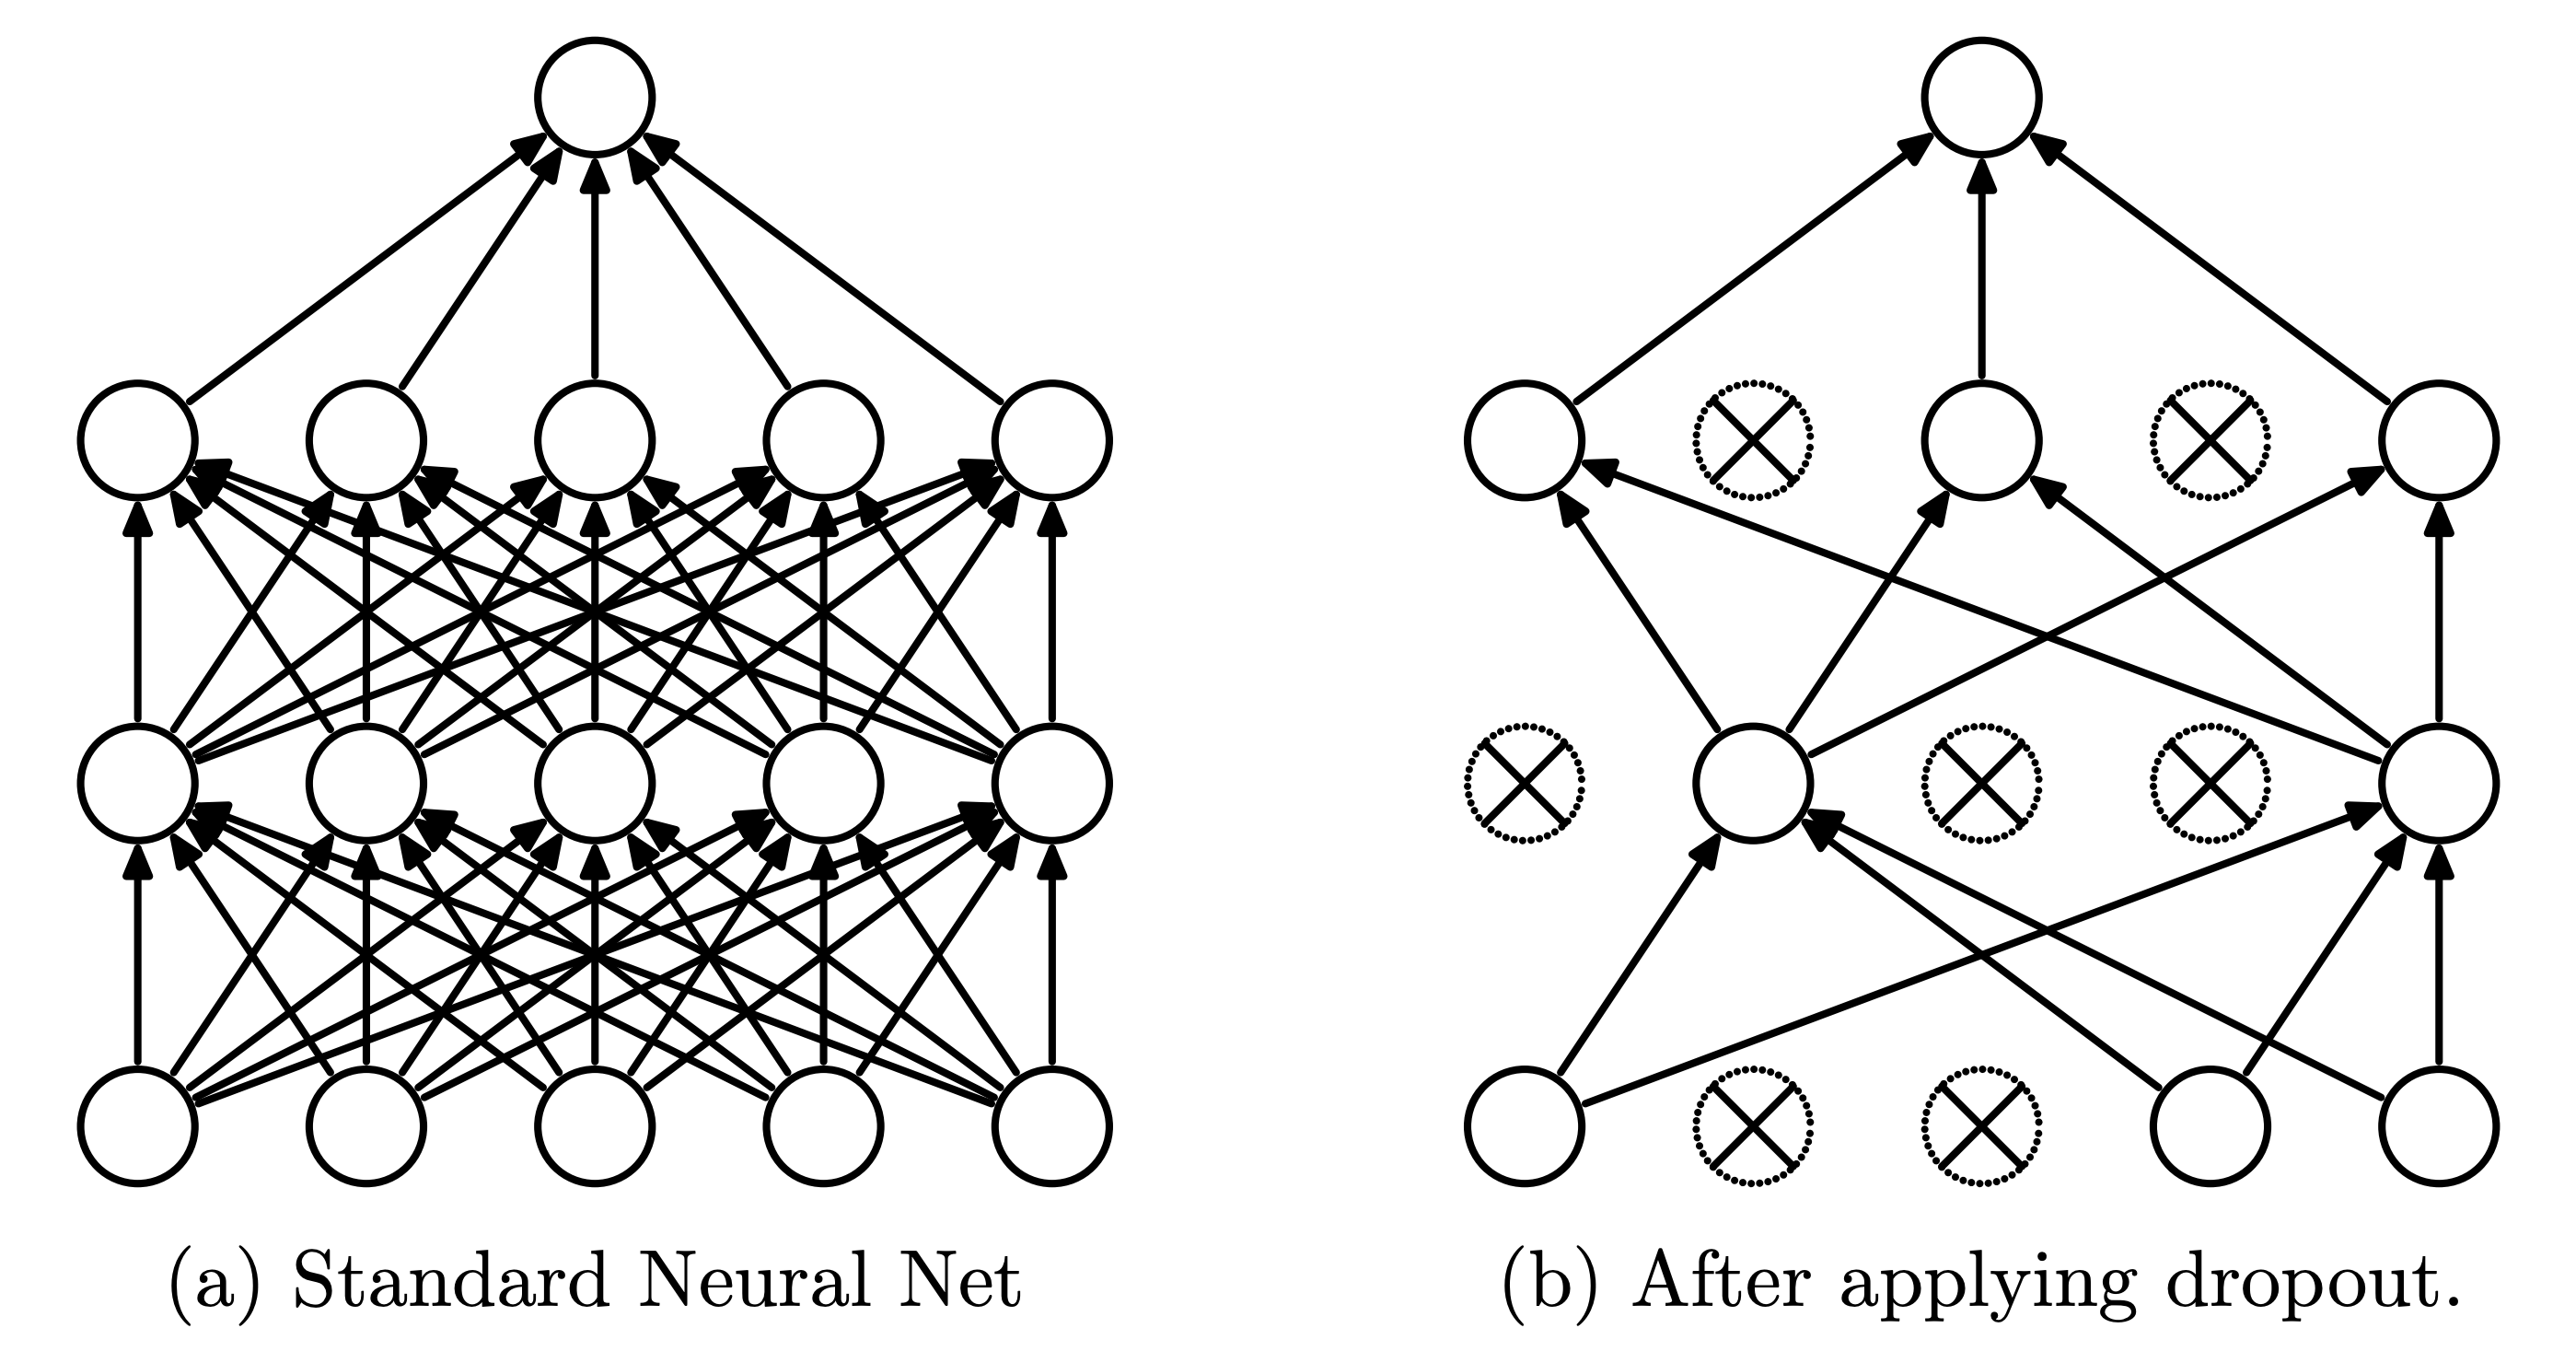
\includegraphics[width=0.7\textwidth]{dropout}
    \caption{Illustrated example of dropout (from \textit{Srivastava, Nitish, et al. ”Dropout: a simple way to prevent neural networks from overfitting”, JMLR 2014})}
    \label{fig:dropout}
\end{figure}

Figure \ref{fig:dropout} shows and example of dropout applied to a simple dense neural network. The idea behind dropout is that the network cannot rely on the features of each individual neuron, because if an essential neuron is shut down, then the network is not able to perform well. By ignoring some percentage of different neurons at each training step, the model is forced to learn more robust features, that work well together with the features of other groups of neurons. This approach prevents co-adaption, which is a situation that arises when some neurons are highly dependant on others. Dropout forces each single neuron to learn informative features, different from the ones learned by other neurons. In this way, a neuron is not dependant on the features of few individual neurons, leading to a better generalization.


\subsection{Convolutional neural network}
\paragraph{} Convolutional neural networks (\acsp{cnn}) are feed-forward networks that work very well especially for image recognition and complex visual tasks in general \cite{OReilly:handsonML}. A typical \acs{cnn} architecture consists of different building blocks: the convolutional layers, which identify low-level features in the image and learn to assemble them into higher-level features; the pooling layers, which subsample the image in order to reduce its dimensionality; finally, the dense network, which is at the end of the architecture and that uses the extracted features to make a prediction (see Figure \ref{fig:nn_conv}). Let's look at the functioning of convolutional and pooling layers.
\begin{figure}[htbp]
    \centering
    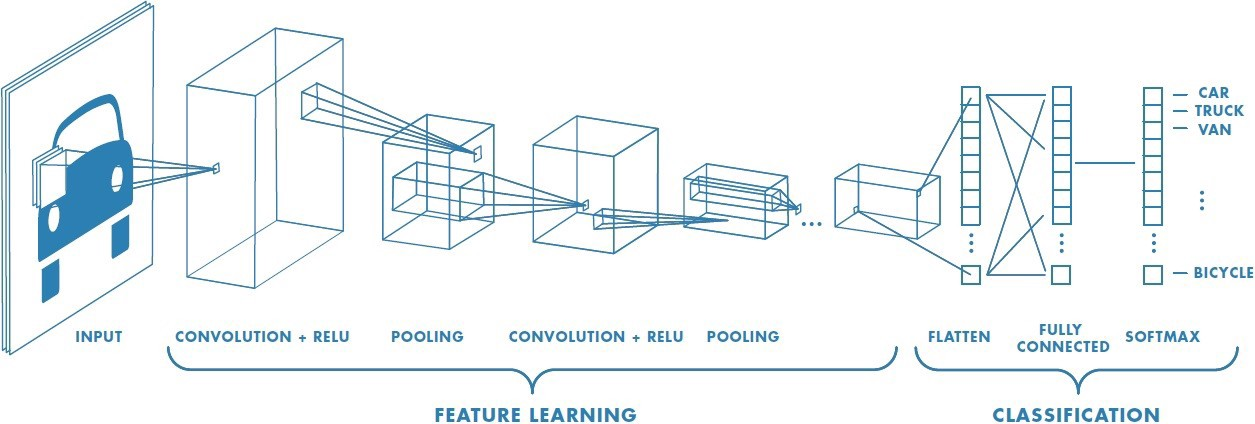
\includegraphics[width=1\textwidth]{nn_conv}
    \caption{Typical architecture of a convolutional neural network (from \textit{Medium - Towards Data Science})}
    \label{fig:nn_conv}
\end{figure}

Convolutional layers are different from dense layers only for the fact that they are not fully-connected: in convolutional layers, neurons are not connected to all previous layer's neurons, but only to neurons in their receptive fields. If we represent one layer's neurons mapped in 2D as a matrix, we can say that each neuron in the current matrix $l$ looks at a limited region of the previous matrix $l-1$, so it is connected only to neurons located within that region, as shown in Figure \ref{fig:nn_conv_layer}. This architecture allows to focus on low-level features in the first layer, where neurons look at small regions of the input image, and to aggregate them in high-level features in the following layers, where neurons combine lower-level features form the previous layer.
\begin{figure}[htbp]
    \centering
    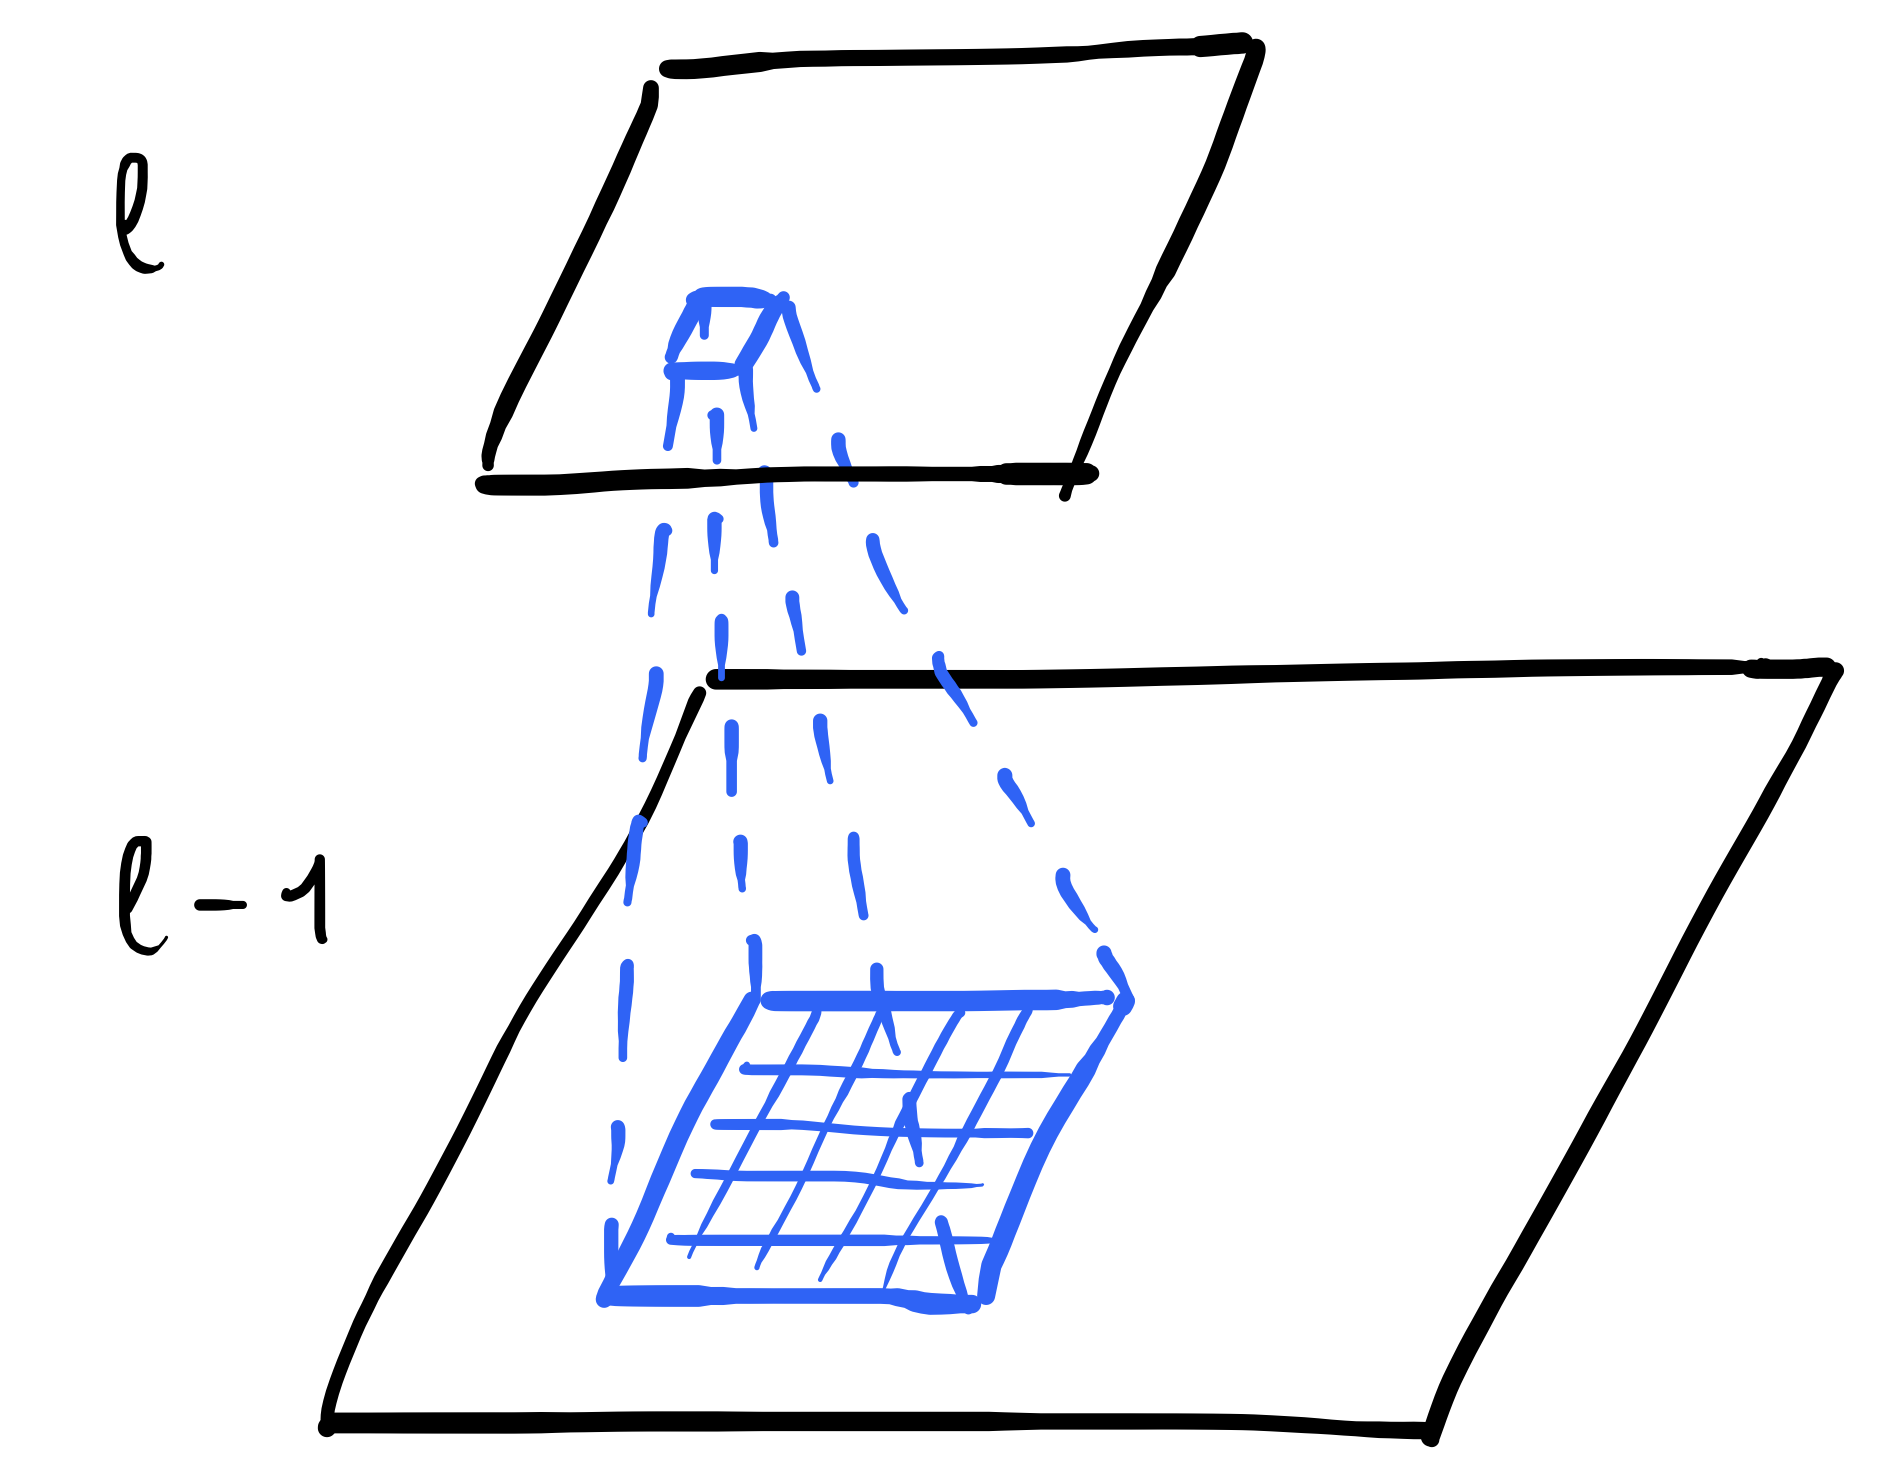
\includegraphics[width=0.35\textwidth]{nn_conv_layer}
    \caption{Relation between convolutional layer's neurons}
    \label{fig:nn_conv_layer}
\end{figure}

\begin{figure}[htbp]
    \centering
    \begin{subfigure}[t]{0.25\textwidth}
		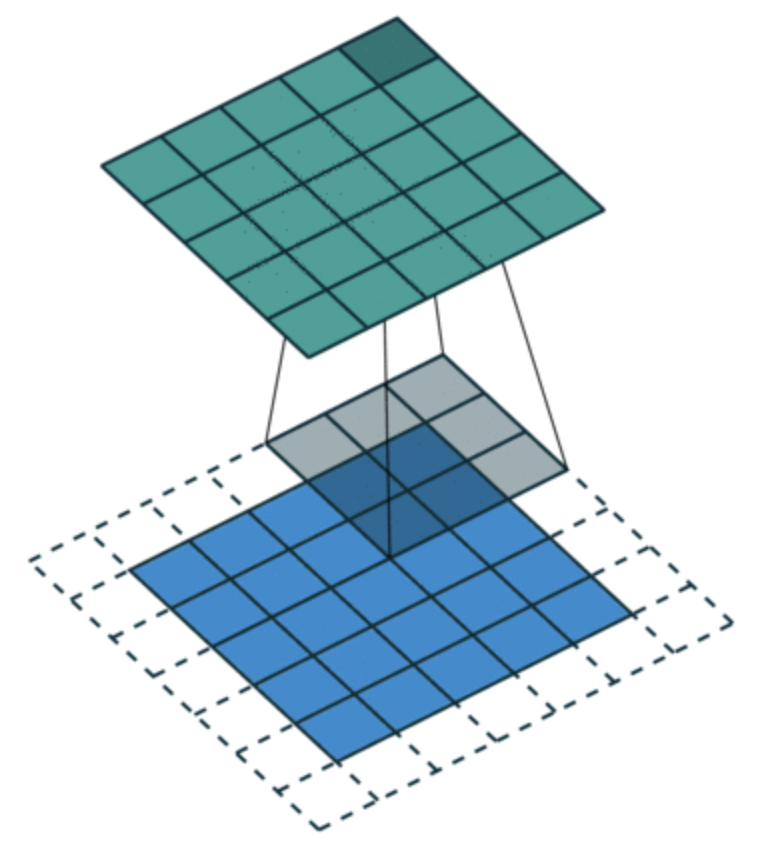
\includegraphics[width=1\textwidth]{nn_conv_padding}
        \caption{Zero padding}
        \label{fig:nn_conv_padding}
	\end{subfigure}
	~
	\begin{subfigure}[t]{0.8\textwidth}
		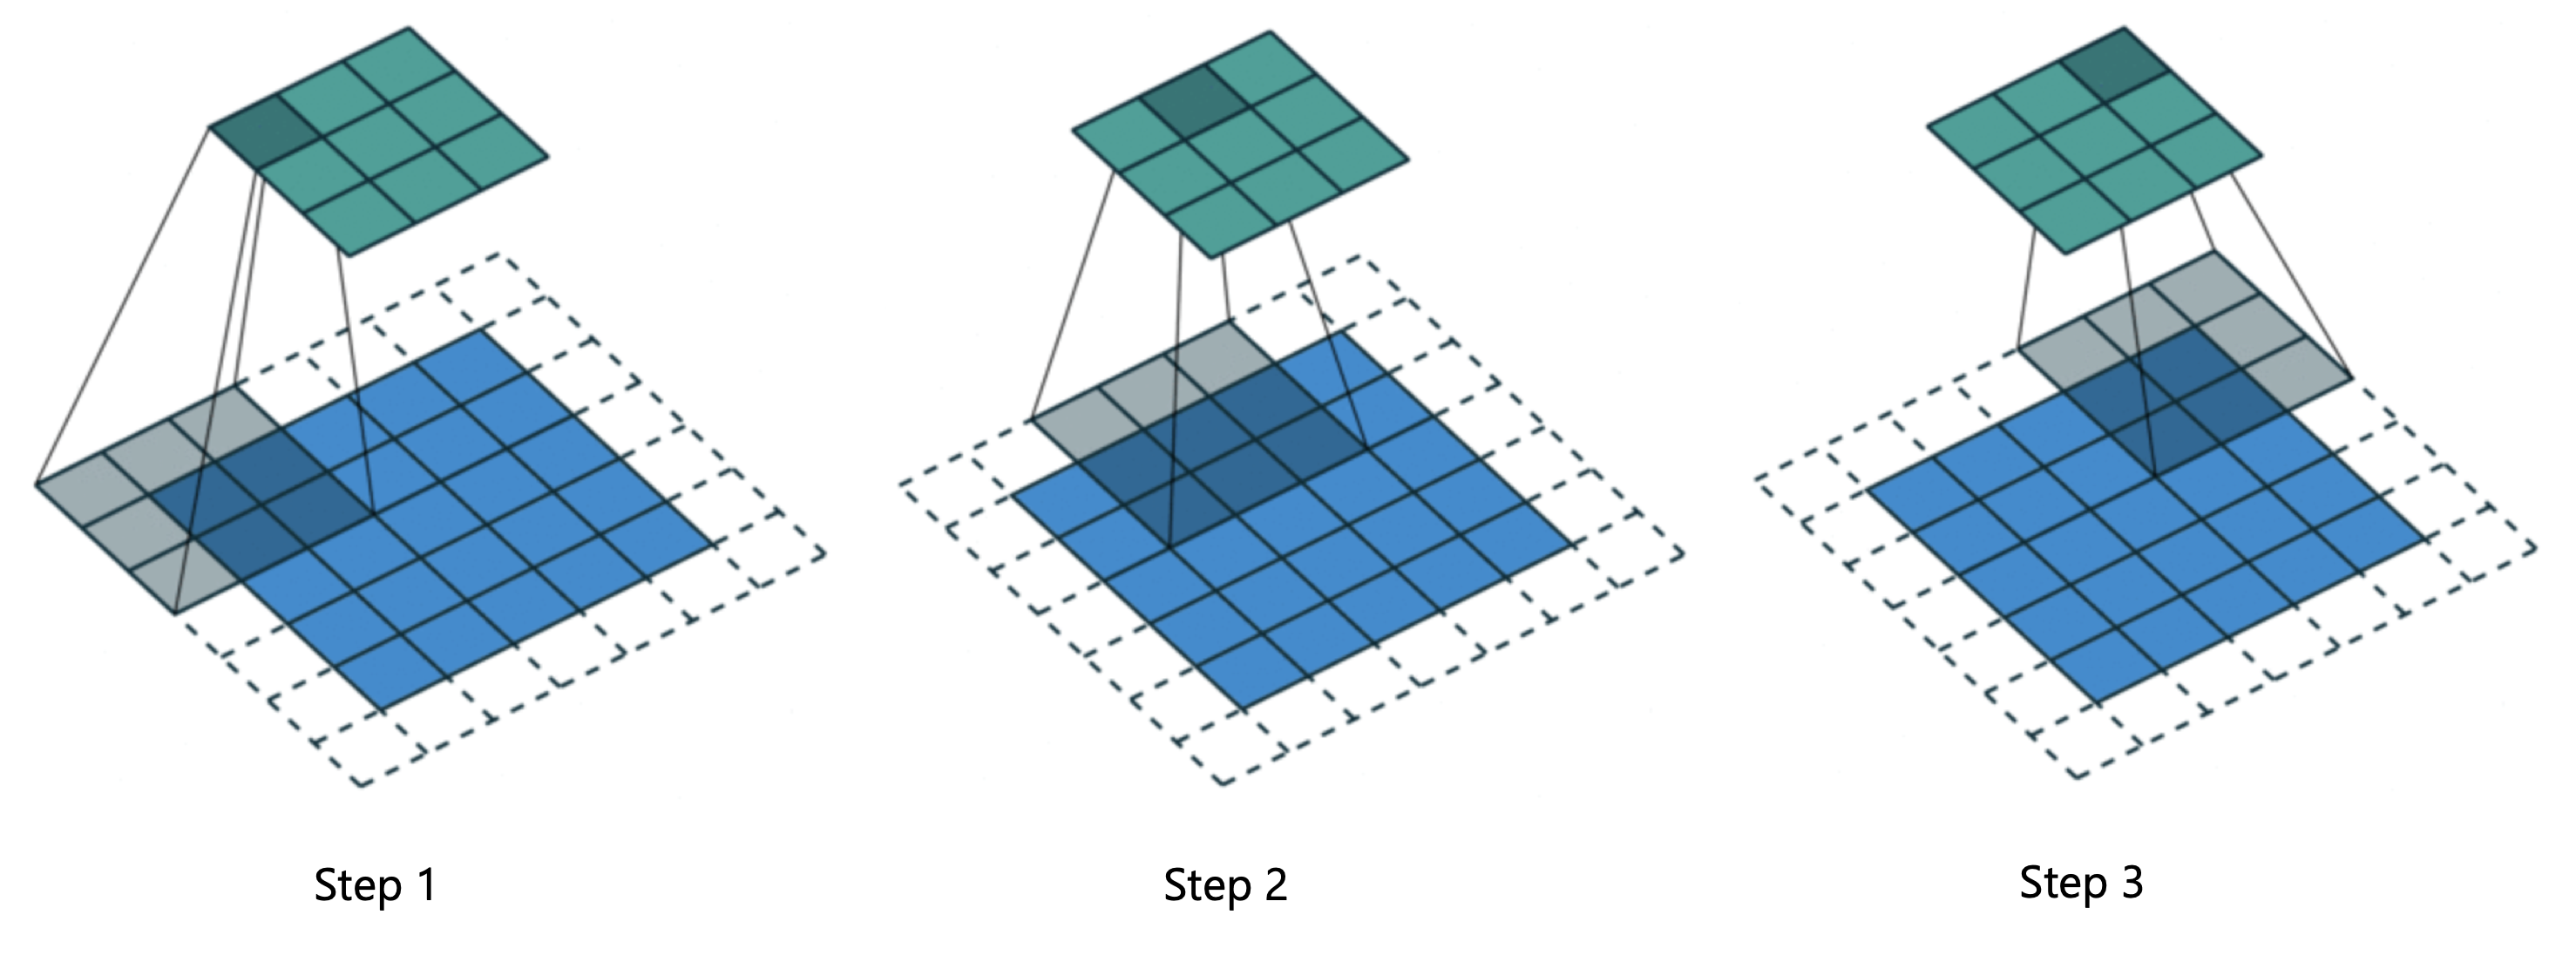
\includegraphics[width=1\textwidth]{nn_conv_stride}
        \caption{Sequence of receptive fields with stride equal to 2}
        \label{fig:nn_conv_stride}
    \end{subfigure}
    \caption{(from \textit{Medium - Towards Data Science})}
    \label{fig:padding_stride}
\end{figure}

In order for a layer to have the same dimensionality of the previous layer, zero padding can be applied by adding a zero-frame to the previous layer (Figure \ref{fig:nn_conv_padding}). In order for a layer to have a much smaller dimensionality with respect to the previous layer, we can use a higher stride, which is the distance between two subsequent receptive fields. By default, the stride is set to 1, so usually the difference between two receptive fields is is one row/column of neurons; by increasing the stride, a smaller number of receptive fields is taken into consideration, therefore the following layers is much smaller (Figure \ref{fig:nn_conv_stride}).

In a convolutional layer, neurons weights are represented by \textit{filters} (also called \textit{kernels}). A filter is a matrix of the same size of the receptive field and it contains the weights that are applied to the corresponding receptive field. The application of the same filter to all the receptive fields of an image produces a feature map, which identify and highlight the details of the image that are most similar to the filter. A convolutional layer is composed by several feature maps of equal size, that in practice corresponds to having multiple matrices of neuron stacked together generating a third dimension, which is the number of feature maps. In a convolutional layer, all neurons in the same feature map share the same weights and bias, so they all use the same filter, while from layer to layer the filter used is different. In this way, the convolutional layer applies different filters to the input image and each feature map can specialize on identifying a specific image feature. Figure \ref{fig:nn_conv_filter} shows a $3\times3$ filter applied over three feature maps (depth); for example, it could be the case of a color image composed of three color channels, which correspond to the three feature maps.
\begin{figure}[htbp]
    \centering
    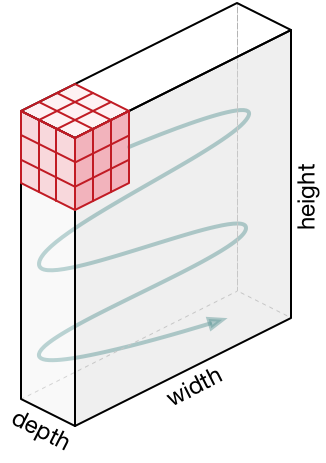
\includegraphics[width=0.3\textwidth]{nn_conv_filter}
    \caption{Movement of a $3\times3$ filter applied over three feature maps (from \textit{Medium - Towards Data Science})}
    \label{fig:nn_conv_filter}
\end{figure}

Convolutional layers are usually followed by pooling layers. As already mentioned, the goal of a pooling layer is to subsample the input image in order to reduce its dimensionality; this action has the positive effects of cutting down the computational and memory loads and of reducing the number of parameters, thus diminishing the risk of overfitting. A pooling layer is very similar to a convolutional layer, since it is focused on a receptive field too and it has configurable size, padding and stride. The crucial difference is that a pooling layer does not have weights, but instead it aggregates all the information in a receptive field by using an aggregation function (for example the mean or max functions). The pooling layer works on every channel (or feature map) independently, so the output has the same depth as the input. The advantage of using a pooling layer also results from the added capability of the model’s invariance to local translation. This means that, since the pooling layer outputs a summarized version of the features detected in a certain area of the input, a small translation of the input generate almost no change in the pooled output.

Through convolutional and pooling layers, a \acs{cnn} is able to learn high-level features, while reducing the data dimensionality, and to use this information to make predictions through the dense neural network at the end of the architecture.


\subsection{Recurrent neural network}
 \paragraph{} Recurrent neural networks (\acsp{rnn}) are usually used to analyze sequences of data and time series in order to predict the future, thanks to their ability to "memorize" past information \cite{OReilly:handsonML}. This is due to the fact that they are not feed-forward network, since the output of a neuron is sent back to itself. In other words, at each time step $t$, a recurrent neuron receives the features of the input $x_t$ as well as its own output $y_{t-1}$ from the previous time step. In this way, each input of a recurrent neuron is determined by the current input instance alongside with some information from all the previous instances. Expanding this logic to an entire layer of recurrent neurons, at each time step $t$, each neuron receives both the input $x_t$ as well as the entire layer's output $y_{t-1}$ from the previous time step. Figure \ref{fig:nn_recurrent} illustrates the logic behind a recurrent neural network, showing the network unrolled through time.
\begin{figure}[t]
    \centering
    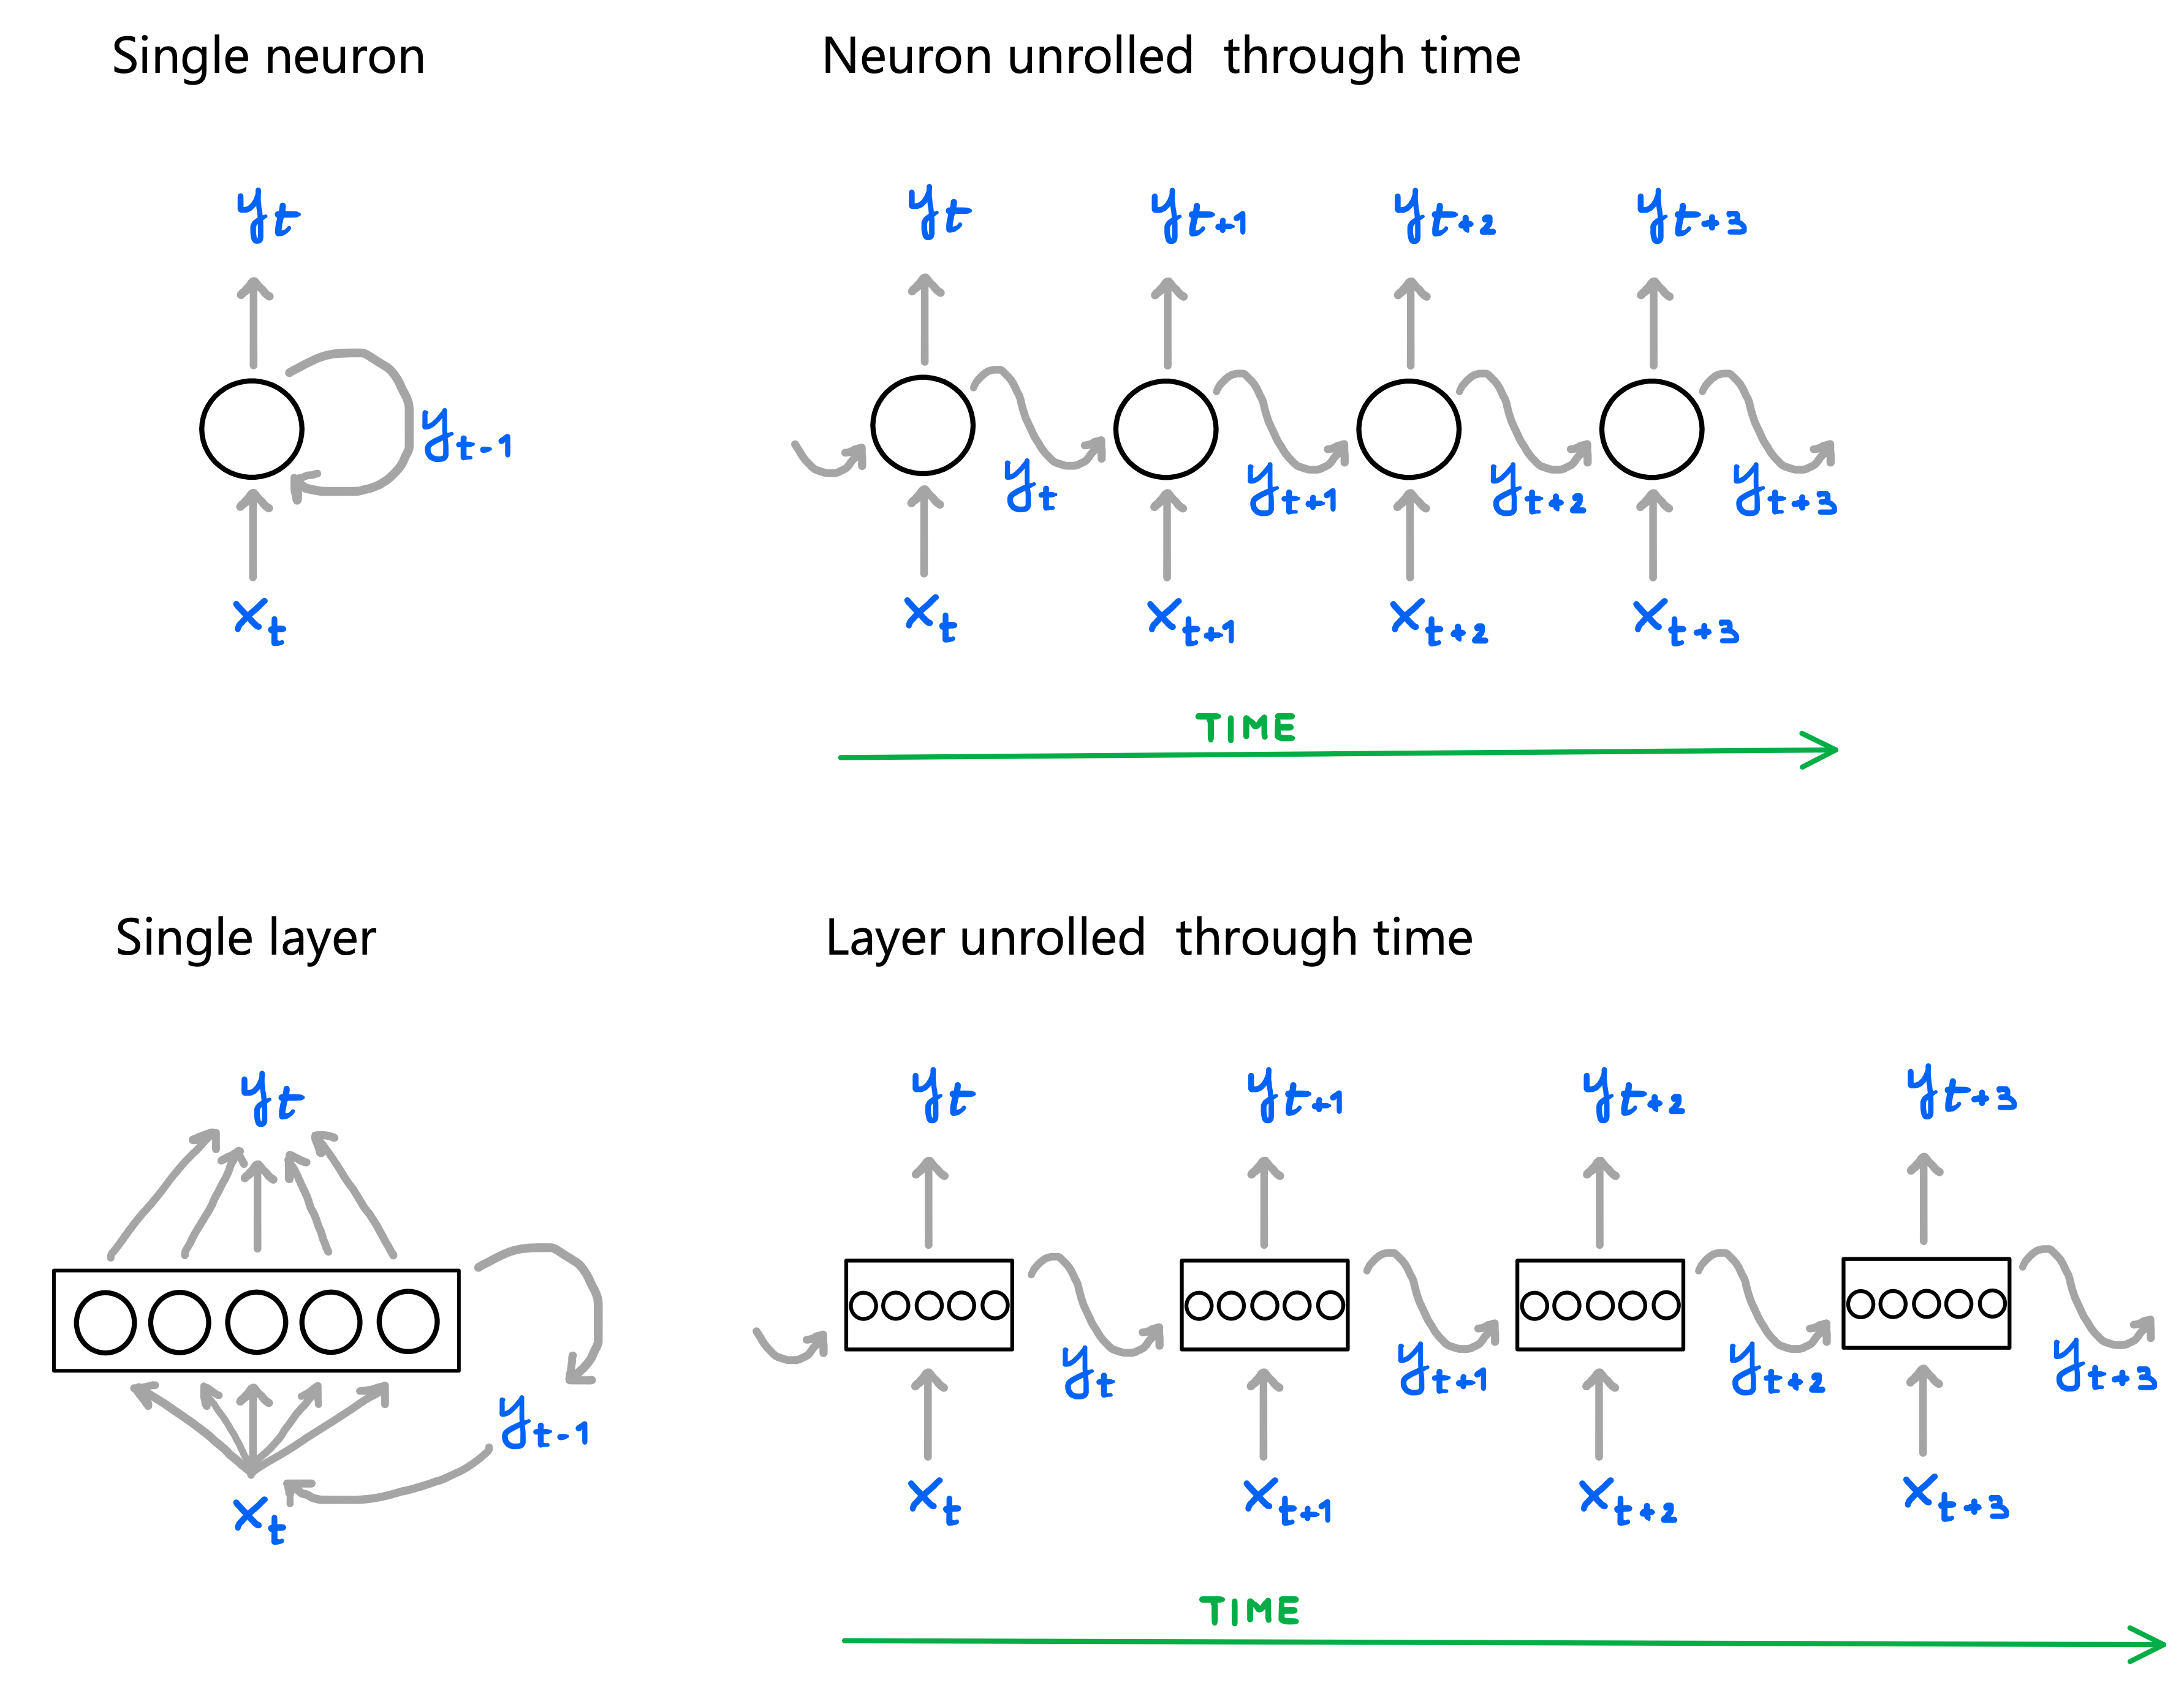
\includegraphics[width=1\textwidth]{nn_recurrent}
    \caption{Logic behind a recurrent neural network}
    \label{fig:nn_recurrent}
\end{figure}

Each recurrent neuron has two sets of weights, one for the inputs $x_t$ and the other for the previous output $y_{t-1}$. Naming $\mathbf{W}_x$ and $\mathbf{W}_y$ respectively these two sets of weights, we can rewrite the equation for the output $\mathbf{Y}_t$ of a recurrent layer:
\begin{align}
    \mathbf{Y}_t = \phi (\mathbf{X}_t \mathbf{W}_x + \mathbf{Y}_{t-1} \mathbf{W}_y + \mathbf{b})
\end{align}
where $\phi$ is the activation function of the layer and $\mathbf{b}$ is the bias. Concatenating the inputs $[\begin{array}{ll}{\mathbf{X}_t} & {\mathbf{Y}_{t-1}}\end{array}]$ and the weights $\mathbf{W} = \left[\begin{array}{c}{\mathbf{W}_x} \\ {\mathbf{W}_y}\end{array}\right]$, we can rewrite the equation as:
    \begin{align}
        \mathbf{Y}_t = \phi ([\begin{array}{ll}{\mathbf{X}_t} & {\mathbf{Y}_{t-1}}\end{array}] \mathbf{W} + \mathbf{b})
    \end{align}

We can say that the network is able to store some sort of "memory" of the past inputs and to use this information for the outputs of the the following time steps. A neuron, or layer of neurons, that is able to preserve some state across time steps is called a \textit{memory cell}. A cell's state at time $t$ can be denoted with $\mathbf{h}_t$, which corresponds to a function $\mathbf{h}_t = f(\mathbf{h}_{t-1}, \mathbf{x}_t)$. In the case of basic memory cells like the ones in a recurrent neural network, the element $\mathbf{h}_{t-1}$ corresponds exactly to the notation $\mathbf{y}_{t-1}$ that we used until now to denote the output from the previous time step.

The standard recurrent neural network model presents some drawbacks. First of all, when the network is trained on long sequences, it may suffer form the vanishing/exploding gradient problem, leading to convergence issues in the training procedure. Moreover, on the long run, the memory of information about the first time steps tends to fade away, since part of the information is lost at each step. We could consider the \acs{rnn} to have a short-term memory, which is not optimal when we need to predict events based on a long sequence of time steps. That is where the \acs{lstm} neural network comes in.


\subsection{\acs{lstm} neural network}
\paragraph{} An \acs{lstm} neural network, differently from a \acs{rnn}, is made of \textit{Long Short-Term Memory} (\acs{lstm}) cells \cite{NeuralComputation:lstm}. This type of cells allows the model to perform much better and to converge faster, in addition to preserving long-term information in long sequences. As shown in Figure \ref{fig:rnn_vs_lstm}, while the standard \acs{rnn} cell contains only a single computational unit (showed as a yellow box), the \acs{lstm} cell contains four interacting units (or layers), each one having a well-defined purpose. An \acs{lstm} cell keeps "in memory" two states, one for the short-term memory and the other for the long-term memory, respectively $\mathbf{h}_t$ and $\mathbf{C}_t$ (also called \textit{cell state}). The first one is the same that we saw for standard recurrent network's cells, while the cell state is what makes the \acs{lstm} model so special.
\begin{figure}[t]
    \centering
    \begin{subfigure}[t]{0.8\textwidth}
		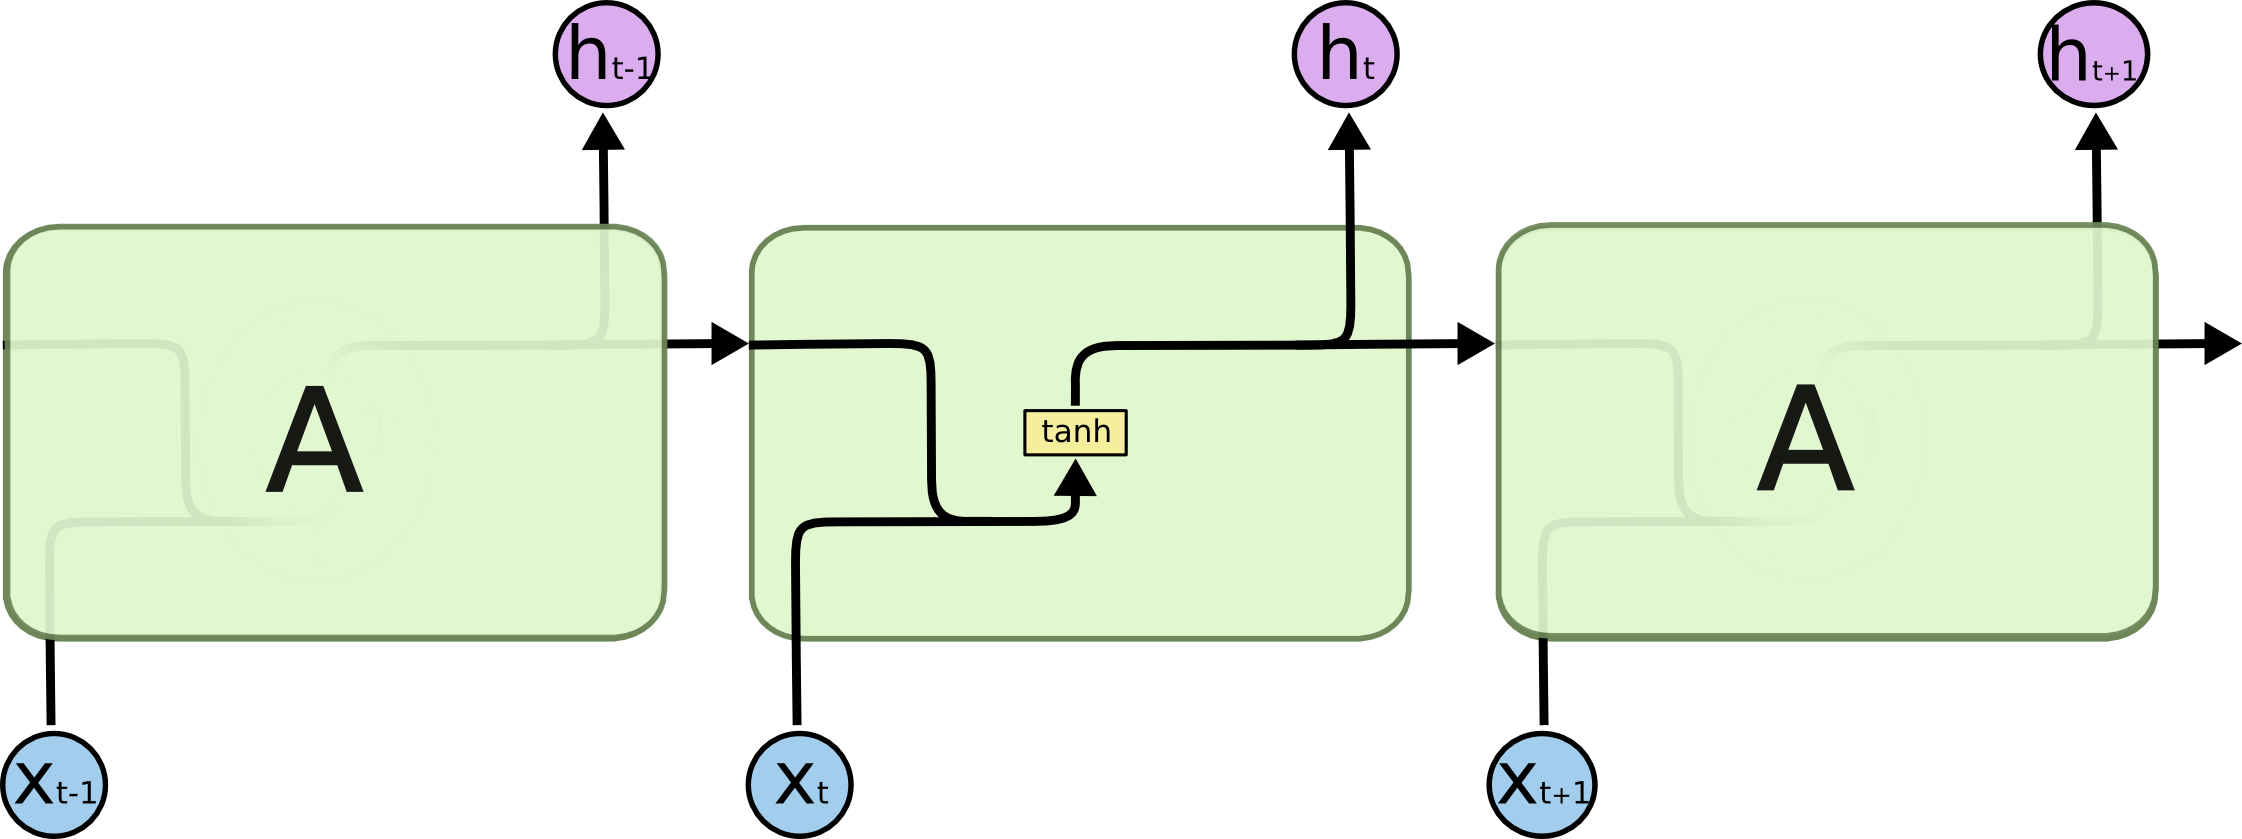
\includegraphics[width=1\textwidth]{nn_simplernn}
        \caption{Standard \acs{rnn} cell}
        \label{fig:nn_simplernn}
	\end{subfigure}
	~
	\begin{subfigure}[t]{0.8\textwidth}
		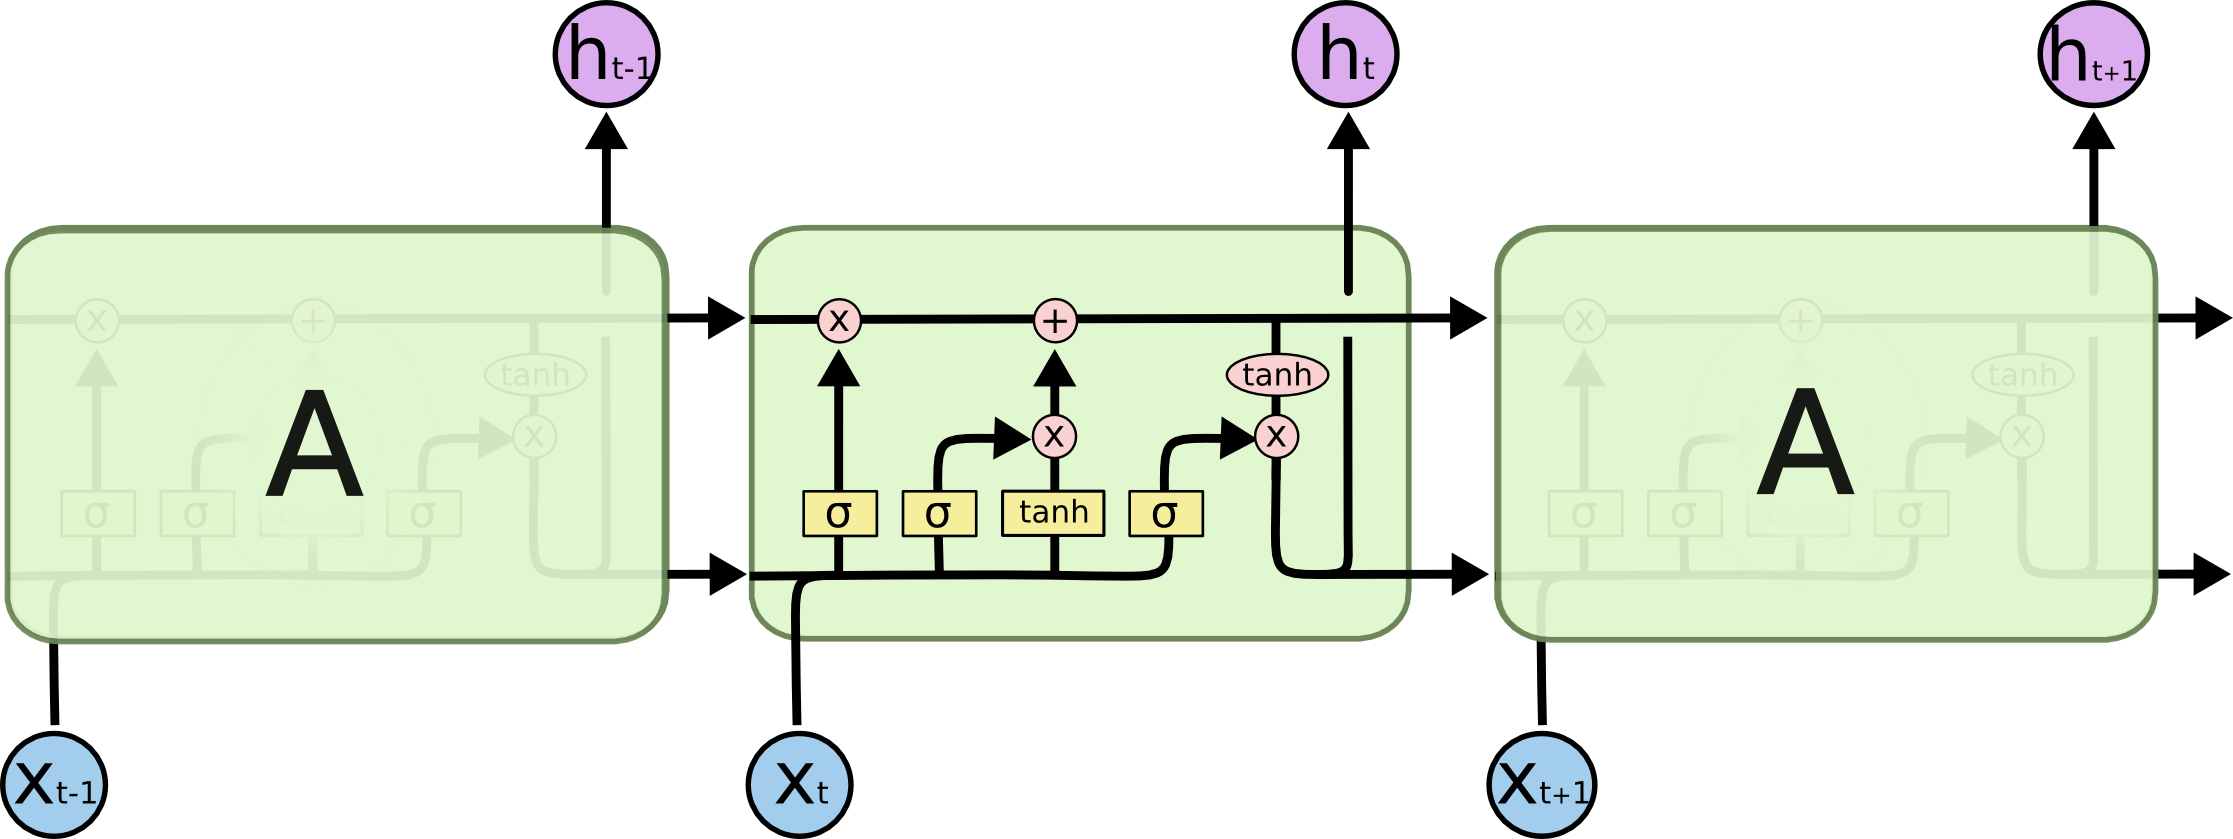
\includegraphics[width=1\textwidth]{nn_lstm}
        \caption{\acs{lstm} cell}
        \label{fig:nn_lstm}
    \end{subfigure}
    ~
    \begin{subfigure}[t]{0.6\textwidth}
		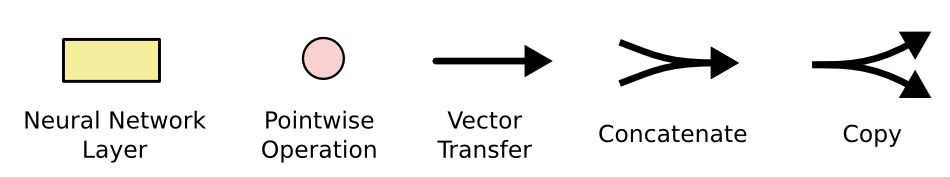
\includegraphics[width=1\textwidth]{nn_lstm_notation}
        \caption{Image notation}
        \label{fig:nn_lstm_notation}
	\end{subfigure}
    \caption{Difference between a standard \acs{rnn} cell and a \acs{lstm} cell (from \textit{colah's blog})}
    \label{fig:rnn_vs_lstm}
\end{figure}

In addition to the three inputs $\mathbf{x}_t$, $\mathbf{h}_{t-1}$ and $\mathbf{C}_{t-1}$, the \acs{lstm} cell makes use of four different fully connected layer, three of them using a sigmoid activation function and the remaining one using a \acs{tanh} activation function. Each one of the sigmoid activation outputs goes through a \textit{gate}, indicated in Figure \ref{fig:rnn_vs_lstm} with the symbol $\otimes$, representing an element-wise multiplication. Gates use the output of the sigmoids (between 0 and 1) to determine how much information should be let through. Let's dive into the functioning of an \acs{lstm} cell.

The cell state allows the network to decide what to store in the long-term memory and what to discard. Traversing the cell from left to right (Figure \ref{fig:nn_lstm_step1}), the cell states goes through two operations, the first being the \textit{forget gate} and the second being and addition operation. The forget state determines which long-term information to drop from $\mathbf{C}_{t-1}$ and it is controlled by the first sigmoid layer's output $f_t$, calculated from $\mathbf{x}_t$ and $\mathbf{h}_{t-1}$ (Figure \ref{fig:nn_lstm_step2}). The addition operation, on the other hand, adds information to the cell state based on the output of the \textit{input gate}, which determines which new information coming from $\mathbf{x}_t$ and $\mathbf{h}_{t-1}$ will be stored in the cell state (Figure \ref{fig:nn_lstm_step4}). The input gate is controlled by the second sigmoid layer's output $i_t$ and by the \acs{tanh} layer's output $\tilde{C}_t$ (Figure \ref{fig:nn_lstm_step3}). After that, the long-term state $\mathbf{C}_t$ is ready to be output, but before that, its state is copied to be passed to a \acs{tanh} activation function and to be filtered by the last gate, which is the \textit{output gate}, controlled by the third sigmoid layer's output $o_t$ (Figure \ref{fig:nn_lstm_step4}). This operation is essential in order to produce the short-term state $\mathbf{h}_t$ to output.

To sum up the fully-connected layer's roles:
\begin{itemize}
    \item The \acs{tanh} layer that outputs $\tilde{C}_t$ takes as inputs $\mathbf{x}_t$ and $\mathbf{h}_{t-1}$ and it is the same that we find in a basic recurrent cell. The result is partially stored as new information in the long-term state.
    \item The sigmoid layer that outputs $f_t$ takes as inputs $\mathbf{x}_t$ and $\mathbf{h}_{t-1}$ and it controls the forget gate. Based on the result, some parts of the long-term state are erased.
    \item The sigmoid layer that outputs $i_t$ takes as inputs $\mathbf{x}_t$ and $\mathbf{h}_{t-1}$ and it controls the input gate. Based on the result, some parts of the new information in $\tilde{C}_t$ are added to the long-term state.
    \item The sigmoid layer that outputs $o_t$ takes as inputs $\mathbf{x}_t$ and $\mathbf{h}_{t-1}$ and it controls the output gate. Based on the result, some parts of the long-term state are read and output as $\mathbf{h}_t$.
\end{itemize}
All the equations for the different outputs can be found in Figure \ref{fig:lstm_steps}.

Through this process, the \acs{lstm} model is able to preserve important information through time and to understand which are the essential inputs to keep and what to discard. This allows the network to learn long-term patterns in the data.
\newpage
\begin{figure}[H]
    \centering
    \begin{subfigure}[t]{0.7\textwidth}
		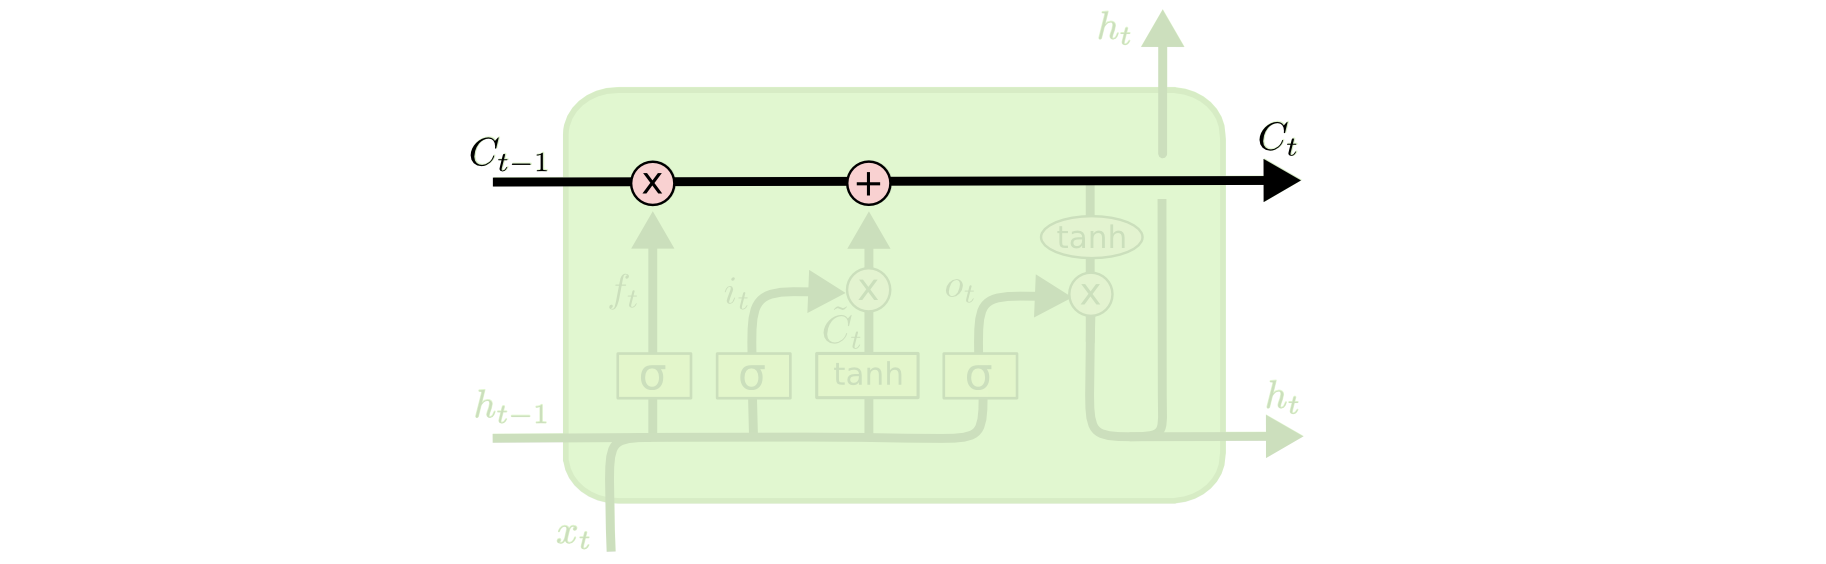
\includegraphics[width=1\textwidth]{nn_lstm_step1}
        \caption{}
        \label{fig:nn_lstm_step1}
	\end{subfigure}
	~
	\begin{subfigure}[t]{0.7\textwidth}
		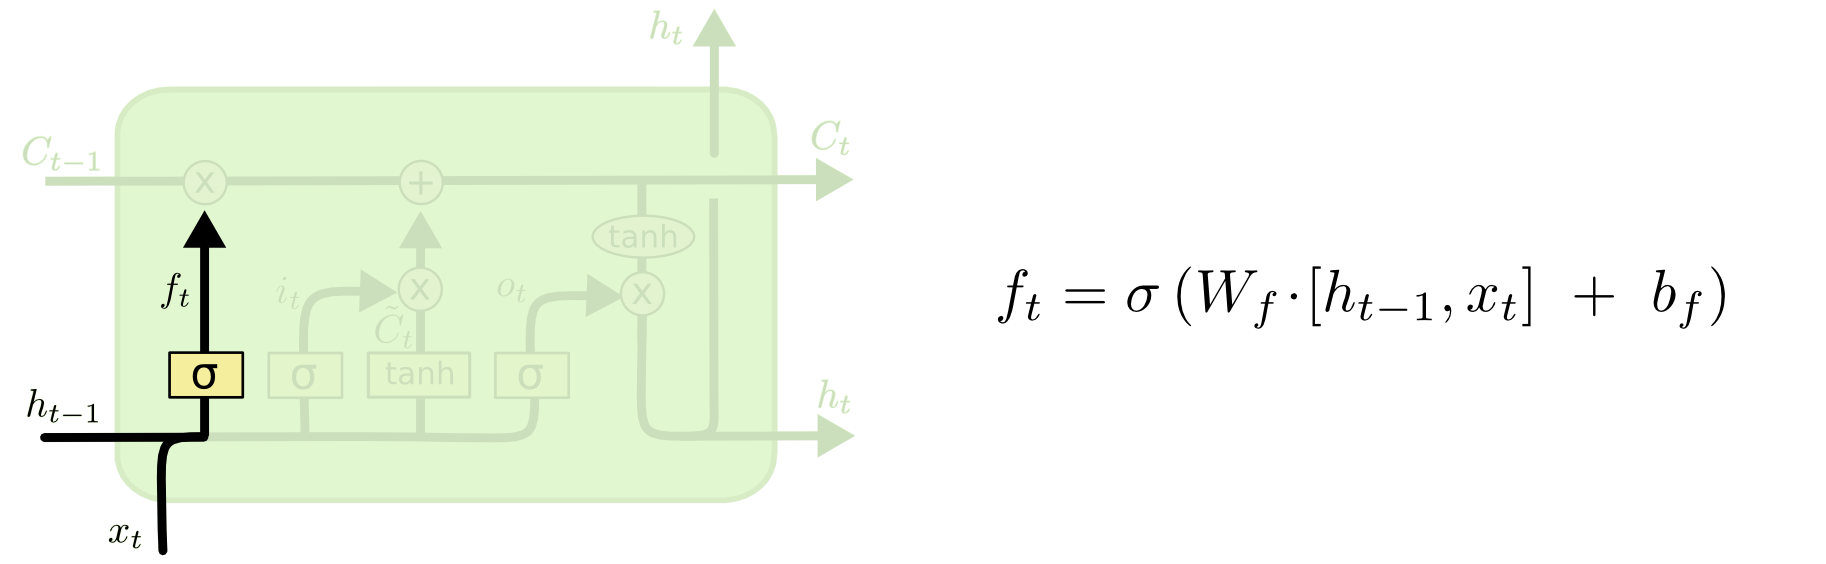
\includegraphics[width=1\textwidth]{nn_lstm_step2}
        \caption{}
        \label{fig:nn_lstm_step2}
    \end{subfigure}
    ~
    \begin{subfigure}[t]{0.7\textwidth}
		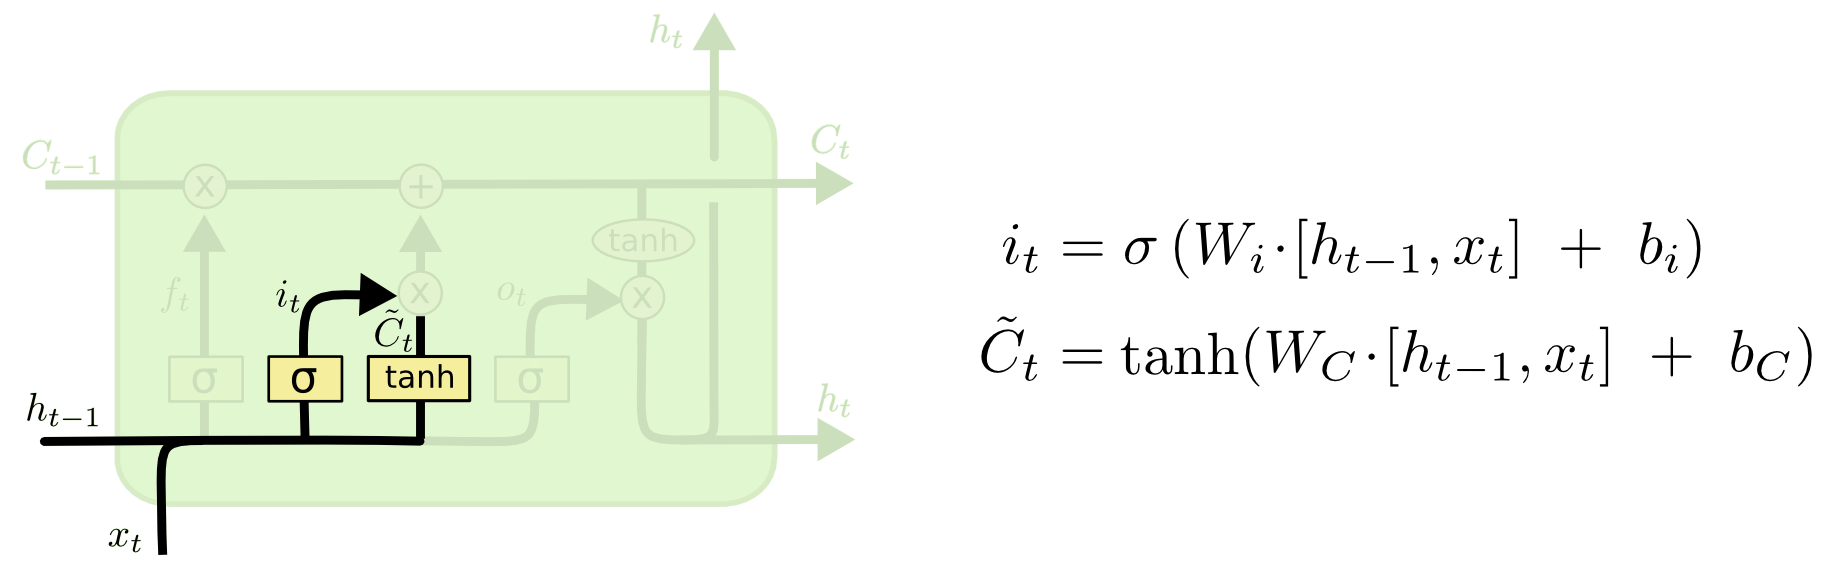
\includegraphics[width=1\textwidth]{nn_lstm_step3}
        \caption{}
        \label{fig:nn_lstm_step3}
    \end{subfigure}
    ~
    \begin{subfigure}[t]{0.7\textwidth}
		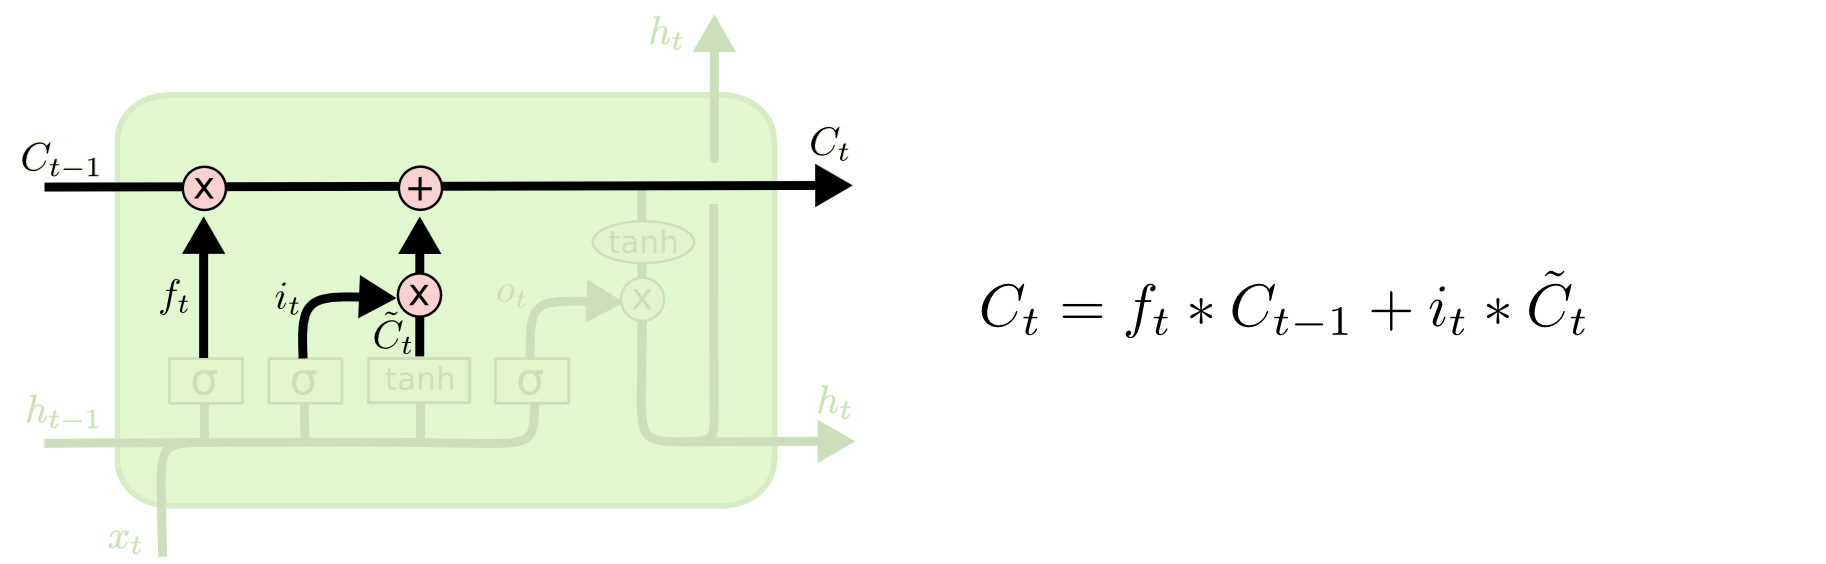
\includegraphics[width=1\textwidth]{nn_lstm_step4}
        \caption{}
        \label{fig:nn_lstm_step4}
    \end{subfigure}
    ~
    \begin{subfigure}[t]{0.7\textwidth}
		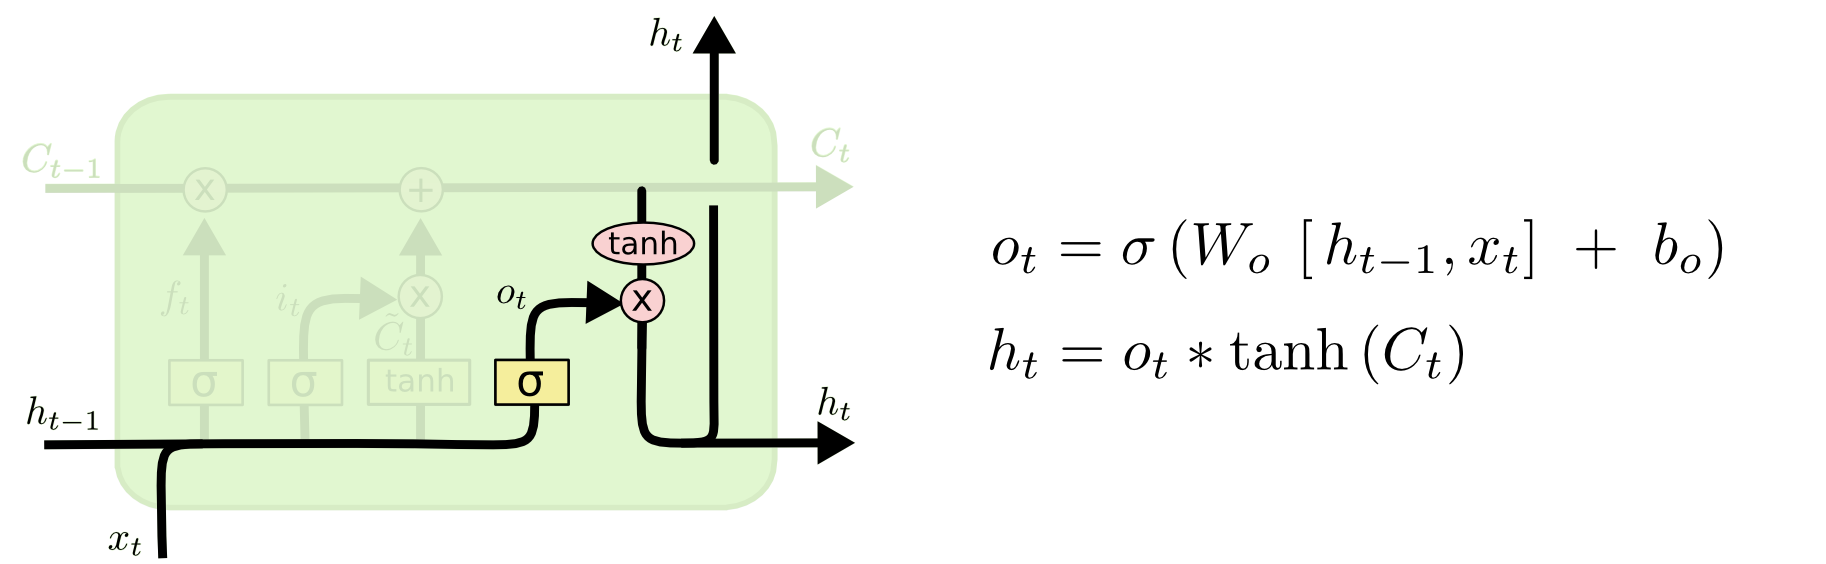
\includegraphics[width=1\textwidth]{nn_lstm_step5}
        \caption{}
        \label{fig:nn_lstm_step5}
    \end{subfigure}
    \caption{Elements in an \acs{lstm} cell step-by-step (from \textit{colah's blog})}
    \label{fig:lstm_steps}
\end{figure}
\newpage

%--------------------------------------------------
% Functional connectivity and graph representation
%--------------------------------------------------

\section{Functional connectivity and graph representation} \label{sec: fc_graphs}
\paragraph{} This section explains some basic knowledge about the functional connectivity of the brain activity and its convenient representation using graphs, which has led to the use of graph-based deep learning models.

Functional connectivity represents the presence of statistical dependencies between the time series of different brain regions \cite{NeurobiologyLanguage:functionalconnectivity}. In other words, functional connectivity measures the relations between time windows of brain activity in different areas of the brain. Assuming that the data respect Gaussian assumptions, these dependencies are usually expressed using covariance or correlation.

In the case of functional \acs{eeg} connectivity, the signal of an electrode represents the brain activity of the brain region in which the electrode is located. We can obtain a sequence of time windows for each brain region's activity by temporally segmenting the signal generated by the electrode located in that region. For instance, if we want to determine the functional connectivity of two brain regions, represented by the electrodes $a_1$ and $a_2$ respectively, we consider their time series $t_{a_1}$ and $t_{a_2}$ and we can compute the Pearson correlation coefficient of the two time series:
\begin{align}
    \textit{corr}_{t_{a_1} t_{a_2}} = \frac{\textit{cov}_{t_{a_1} t_{a_2}}}{\textit{sd}_{t_{a_1}} \cdot \textit{sd}_{t_{a_2}}}
\end{align}
where $\textit{cov}_{t_{a_1} t_{a_2}}$ is the covariance and $\textit{sd}_{t_{a_1}}$ and $\textit{sd}_{t_{a_2}}$ are the standard deviations of the two time series.

Brain's functional connectivity can be properly represented through graphs. A graph is a data structure consisting of nodes and edges. The nodes are entities that hold some sort of information, while the edges are the connections between nodes and they can hold information too. Usually the information held by an edge refer to the relation between the nodes connected by that edge. Graphs are useful to represent non-euclidean data and they can have several properties limiting their flexibility to certain constraints.

In computer science, we can represent a graph with three matrices:
\begin{itemize}
    \item Binary adjacency matrix $\mathbf{A} \in\{0,1\}^{N \times N}$
    \item Node attributes matrix $\mathbf{X} \in \mathbb{R}^{N \times F}$
    \item Edge attributes matrix $\mathbf{E} \in \mathbb{R}^{N \times N \times S}$
\end{itemize}
where $N$ is the number of nodes, $F$ is the number of features for each node and $S$ is the number of edges. The adjacency matrix $\mathbf{A}$ shows the connections between the nodes: the cell at row $i$ and column $j$ contains 1 if there is an edge connecting nodes $i$ and $j$ and it contains 0 otherwise. The node attributes matrix $\mathbf{X}$ contains a row of $F$ features for each node. The edge attributes matrix $\mathbf{E}$ is similar to the adjacency matrix, but instead of containing only ones and zeros, it stores the $S$ attributes of each edge across the third dimension.

A variation of the adjacency matrix is the adjacency matrix with inserted self-loops:
\begin{align*}
    \hat{\mathbf{A}} = \mathbf{A} + \mathbf{I}_N
\end{align*}
where $\mathbf{I}_N$ is an $N \times N$ identity matrix, that is a square matrix with ones on the main diagonal and zeros elsewhere. Another important matrix representing graphs is the degree matrix $\mathbf{D}$, which is a diagonal matrix where each value of the diagonal is the degree of its corresponding node. The degree is the sum of each row of the adjacency matrix.

Functional connectivity can be expressed as a graph by considering each electrode (brain region) as a node and by using the correlation value between electrodes as the attribute of the edges between nodes. In this case, we would obtain a graph having a node for each electrode and an edge for each couple of nodes. In order to reduce the number of edges, we could keep only the most significative ones, that are the ones whose correlation's absolute value is near 1. This representation is able to express the statistical dependencies between brain regions just for a given time instant. In order to introduce the time dimension, we can generate a new graph for each time window, obtaining a sequence of different graphs (see Figure \ref{fig:graph_sequence}). Through this representation, we can see the evolution of brain region dependencies across time, with edges appearing or disappearing based on the correlation value in that time step.
\begin{figure}[htbp]
    \centering
    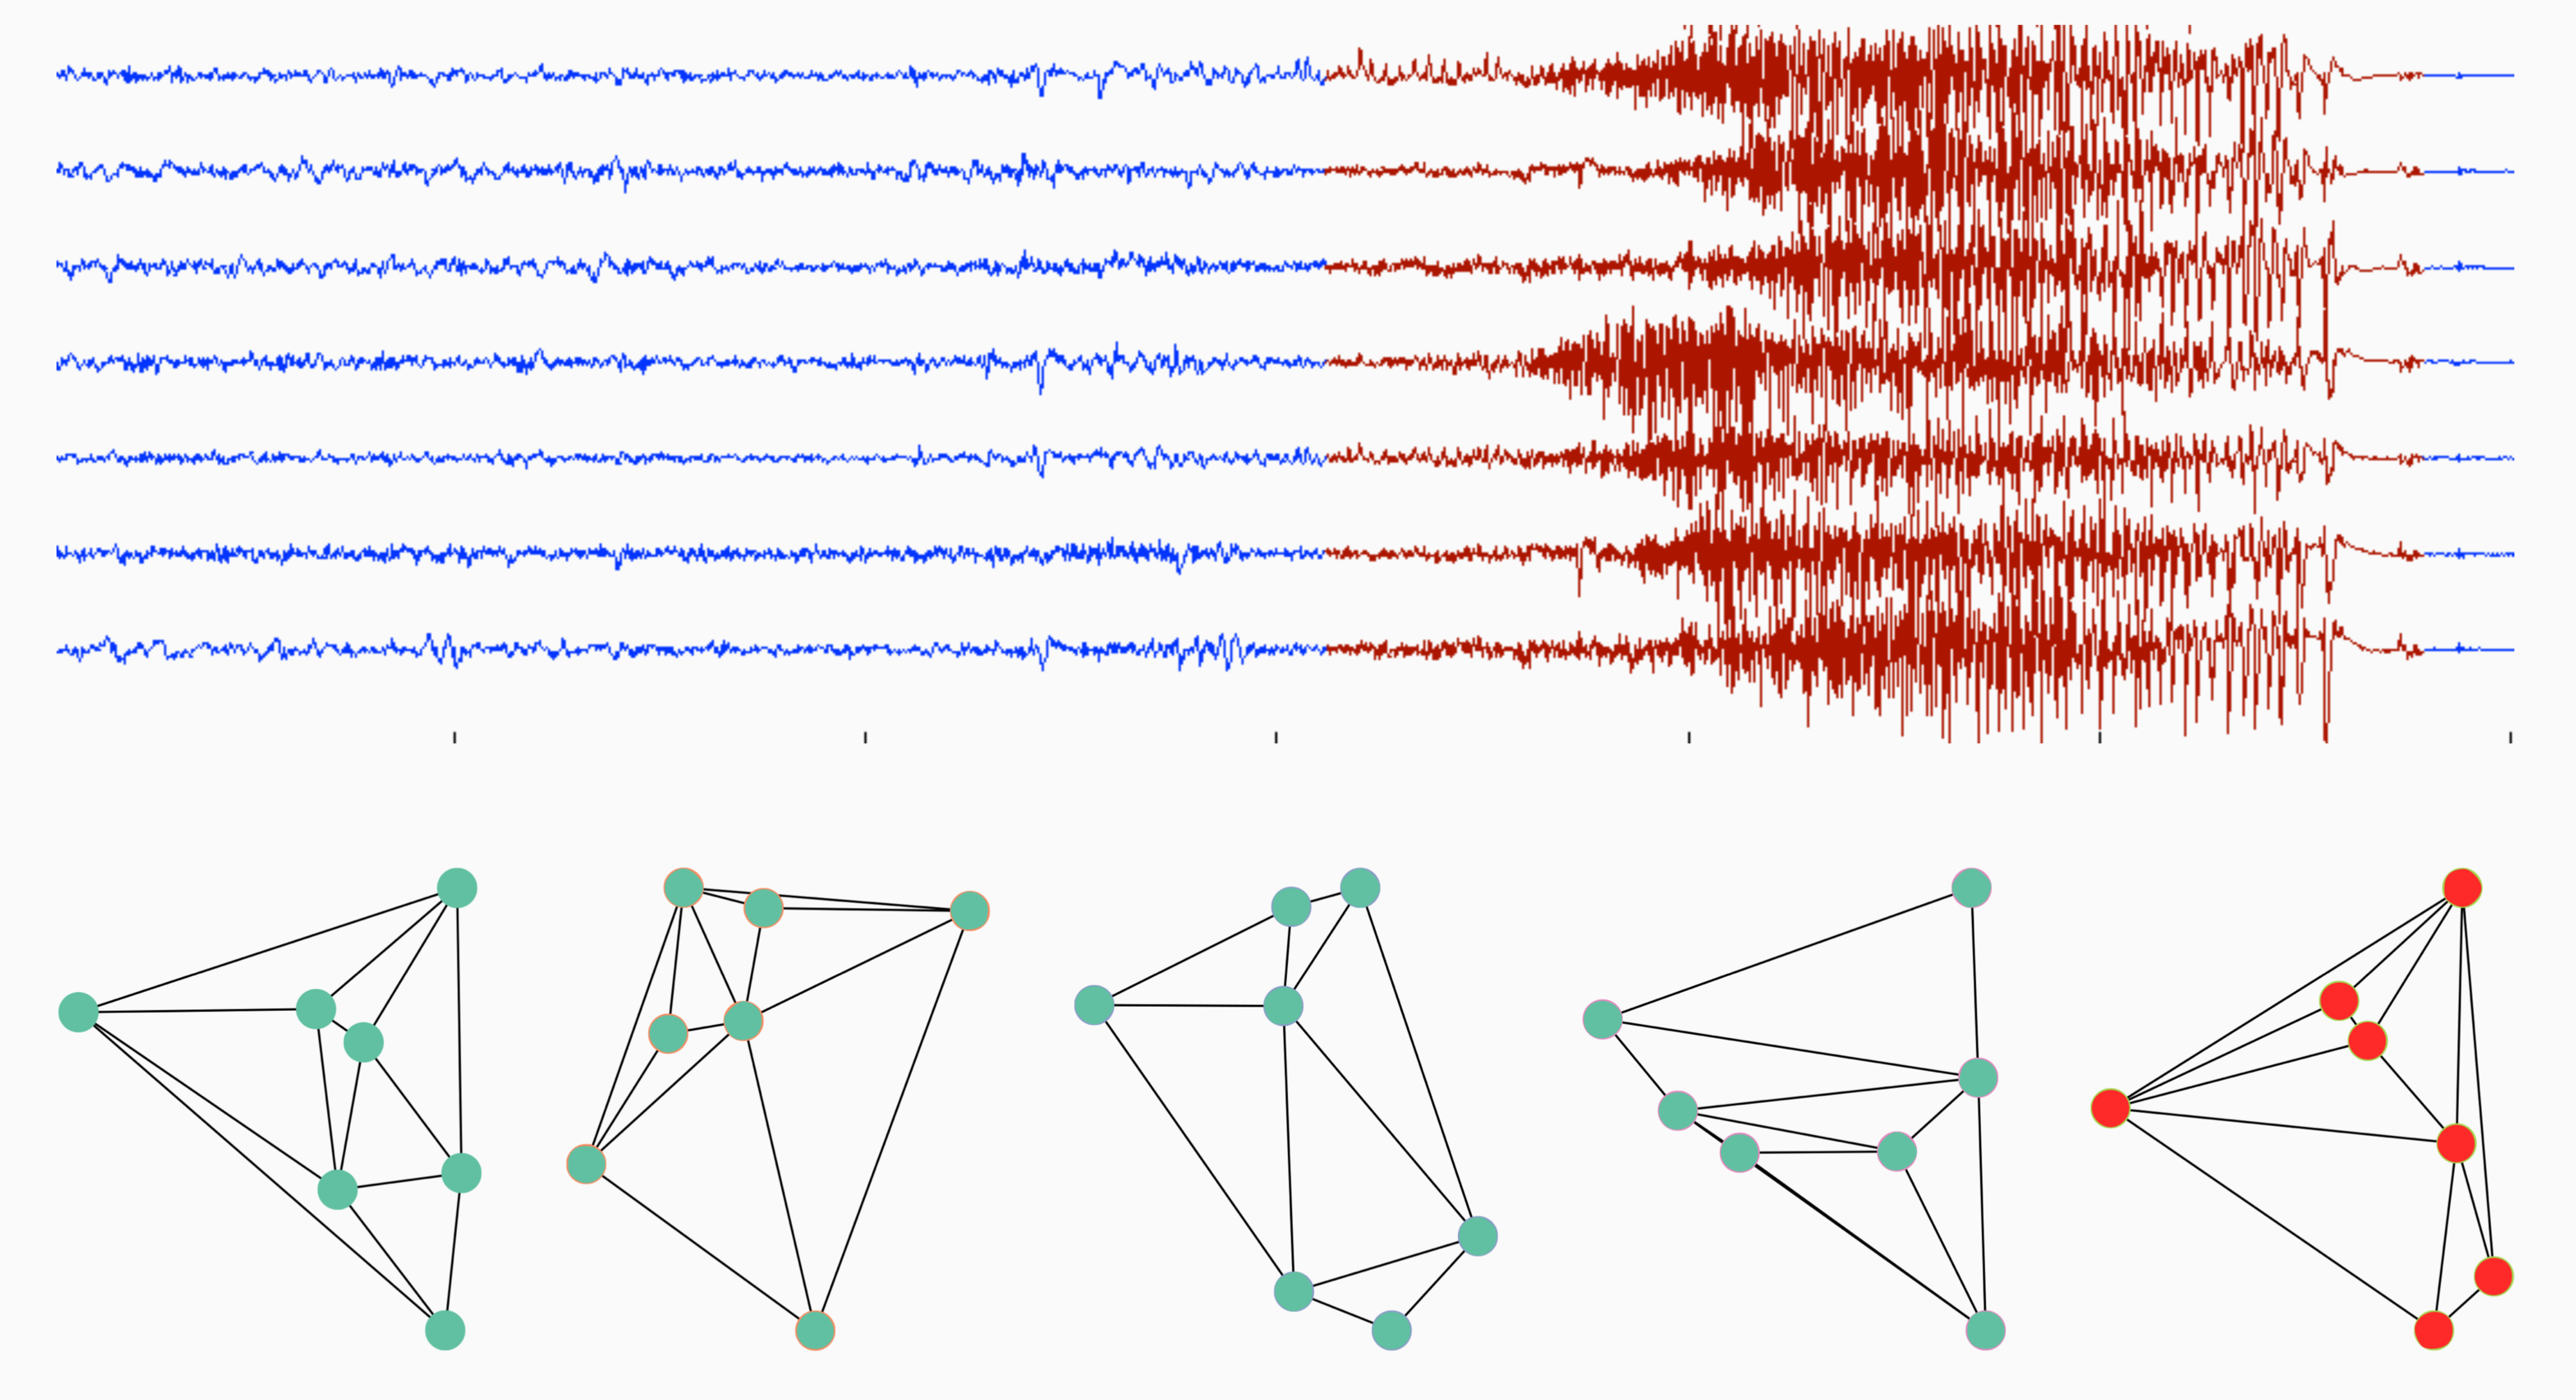
\includegraphics[width=0.8\textwidth]{graph_sequence}
    \caption{Sequence of graphs representing the functional connectivity (from \cite{arXiv:graphstream})}
    \label{fig:graph_sequence}
\end{figure}

%--------------------------------------------------
% Graph-based deep learning models
%--------------------------------------------------

\section{Graph-based deep learning models} \label{sec: graph_dl}
\paragraph{} Geometric deep learning stems from the need to apply deep learning models to non-euclidean data. A lot of research on this topic has been conducted during the last decades in order to develop suitable models for this purpose. One of the most common examples of non-euclidean data is the graph data structure, which is able to encode information about the structure and the relation between entities, while still representing individual features. In order to deal with graph data, graph neural networks (\acsp{gnn}) have been created.

\subsection{Graph neural network and graph convolution} Graph neural networks (\acsp{gnn}) are deep learning models dedicated to working with graph-structured data. They are able to learn from graph information like structure, relationship, connections and individual features of the entities. Their flexibility opens the door to a wide new range of real-world applications, whose data require to take into account the structural information.

One of the most interesting approach to the application of neural networks to graph is the \textit{graph convolution}, which tries to generalize convolutional layers to arbitrary neighbourhoods. The more standard version of convolutional neural networks, indeed, are generally applied to images, where the neighbourhood is determined by the location of the pixels in a 2D space. However, there are situation in which the spatial information is not available and we have to rely on connection between entities in order to define a neighbourhood (just think of molecules or social networks). This is exactly what graph convolution tries to achieve.

Among the most known implementations of graph convolution, there is the \acf{gcn}, from the paper by Kipf and Welling (\cite{arXiv:gcn}). The paper presents a spectral convolutional model applied to graph learning. In a \acs{gcn}, the output of a layer is defined as:
\begin{align}
    \mathbf{X}^{(out)}=\phi\left(\hat{\mathbf{D}}^{-\frac{1}{2}} \hat{\mathbf{A}} \hat{\mathbf{D}}^{-\frac{1}{2}} \mathbf{X}^{(in)} \mathbf{W} + \mathbf{b}\right)
\end{align}
where $\phi$ is the activation function, $\mathbf{b}$ is the bias, $\mathbf{W}$ is the matrix of model's weights, $\mathbf{X}$ is the node attribute matrix, $\tilde{\mathbf{A}}$ is the adjacency matrix with inserted self-loops, computed as $\tilde{\mathbf{A}} = \hat{\mathbf{D}}^{-\frac{1}{2}} \hat{\mathbf{A}} \hat{\mathbf{D}}^{-\frac{1}{2}}$, and $\hat{\mathbf{D}}$ is the degree matrix computed from $\hat{\mathbf{A}}$.

\subsection{Edge-conditioned convolution}
\paragraph{} The graph convolution is able to filter the node features based on the adjacency matrix, but it does not take into account the edge attributes matrix. The \textit{edge-conditioned convolution} (\acs{ecc}) address this issue by replacing the model's weights with a neural network that transforms the edge features into convolutional kernels (\cite{arXiv:eccn}). The resulting formula for a single node is:
\begin{align}
    \mathbf{X}^{(out)}_i=\phi\left(\frac{1}{\mathcal{N}(i)} \sum_{j \in \mathcal{N}(i)} \mathbf{X}^{(in)}_j f(\mathbf{E}_{ji}) + \mathbf{b}\right)
\end{align}
where $\mathcal{N}(i)$ are the one-step neighbourhood of node $i$, $\mathbf{E}$ is the edge attributes matrix and $f(\cdot)$ is a dense neural network that output the convolution kernel as a function of $\mathbf{E}$.

\subsection{Global pooling}
\paragraph{} Like in standard convolutional neural networks, the convolution on graph is usually followed by a pooling layer to get more general features. The problem with the generalization of local pooling layer is that in graph there is no locality as in images. For this reason, the most common approach is to use a global pooling layer on the graph's node features, which reduces the representation of the graph to a single "virtual" node that summarizes all the features of all the original nodes in the graph. This is usually placed after all the convolutional layer, just before the dense neural network for the final prediction.

A global pooling layer aggregates all the node features through an aggregation function (i.e. mean, sum, max functions). For this project, global average pooling has been used, which is defined as:
\begin{align}
    out^{(l)} = \frac{1}{N^{(l)}} \sum_{i=1}^{N^{(l)}} \mathbf{X}^{(l)}_i
\end{align}

The downside of this approach is that, while summarizing the node features, the global pooling layer isn’t able to preserve the graph’s topological information. In order to take into account also the structure of the graph, hierarchical pooling layers have been proposed lately. They are able to coarsens the graph by dropping some of its nodes based on a measure of the importance of the nodes, thus down-sampling the graph representation.

\subsection{Graph-based LSTM and convolutional neural networks}
\paragraph{} For the purpose of this project, graph convolution has been used as a preprocessing tool in order to extract features from the graph data. The graph-conv-pool block, composed by a graph convolutional layer and a global pooling layer, can be followed by any standard neural network, such as dense, convolutional and \acs{lstm} neural networks. With this configuration, the role of the graph-conv-pool block is simply to deal with the graph structure of the data and to extract structural features in a form that can be processed by standard models.

\section{State-of-the-art in seizure prediction}

\todo[inline]{The following part is taken by old chapter 3 - you can reuse it by adapting it in this section}
\paragraph{} Once we identified the problem, we spent some time inquiring about previous approaches to the problem. With this aim, we read several scientific papers about seizure prediction in order to find out which methods have been already used and the level of performance they obtained. Through this research, we realized how complex was the problem and how difficult it was to obtain good results, even using powerful deep learning models. We also found out that, in order to have acceptable results, the majority of these models needed to be trained on a large amount of data, which in the case of epileptic seizures is difficult to gather.\clearpage
%************************************************
% METHODS
%************************************************

\chapter{Methods} \label{chap: methods}

\paragraph{} \textit{This chapter provides a high-level overview of the work that has been done for this project and the process that has been used.}

%------------------------------------------------
% Overview of the project steps
%------------------------------------------------

\section{Overview of the project steps} \label{sec: overview_project_steps}
\paragraph{} The work done for this master thesis project can be summarized via a list of steps we've gone through:
\begin{enumerate}
    \item Definition of the problem to solve;
    \item Research about previous approaches to the problem;
    \item Objective of the project;
    \item Data collection (out of the scope of this project);
    \item Data analysis and familiarization;
    \item Technical definition of the problem;
    \item Choice of the machine learning and deep learning models to use;
    \item Data preprocessing;
    \item Application of the models to the prediction tasks;
    \item Results evaluation;
    \item Conclusions.
\end{enumerate}
The following sections will give a short description of what has been done for each project step.

%------------------------------------------------
% Step 1: Definition of the problem to solve
%------------------------------------------------

\section{Step 1: Definition of the problem to solve} \label{sec: step_definition_problem_to_solve}
\paragraph{} The problem we decided to focus on for this project is the seizure prediction problem, which consists of predicting in advance the happening of an epileptic seizure in a person. The study has been conducted using intracranial electroencephalography data (\acs{ieeg}) and it is devoted to all the people suffering from drug-resistant epilepsy, which are forced to deal with epileptic seizures in everyday life. With the goal of being able to predict epileptic seizures few seconds in advance, the prediction would allow the neurostimulator to intervene in time on the patient brain in order to block the imminent occurrence of the seizure. The possibility to avoid even only a few of the epileptic seizures of a person would already improve by a lot her living standards.

%-----------------------------------------------------------
% Step 2: Research about previous approaches to the problem
%-----------------------------------------------------------

\section{Step 2: Research about previous approaches to the problem} \label{sec: step_research_about_previous_approaches}
\paragraph{} Once we identified the objective problem, we spent some time inquiring about previous approaches to the problem. With this aim, we read several scientific papers about seizure prediction in order to find out which methods have been already used and the level of performance they obtained. Through this research, we realized how complex was the problem and how difficult it was to obtain good results, even using powerful deep learning models. We also found out that, in order to have acceptable results, the majority of these models needed to be trained on a large amount of data, which in the case of epileptic seizures is difficult to gather.

%------------------------------------------------
% Step 3: Objective of the project
%------------------------------------------------

\section{Step 3: Objective of the project} \label{sec: step_objective_project}
\paragraph{} Having a clearer idea of the problem we were going to face and of its level of complexity, we defined the objective of the project and its boundaries. We decided to conduct a study on different machine learning and deep learning models applied to the problem of seizure prediction, generating a review of models to solve this problem and looking for the best configuration for each of them. The common thread we set throughout all the project was the lack of data to train the models. Epileptic seizure data, indeed, are very difficult to gather, so we wanted to find out how well the models would have performed in a real-life scenario, having a very restricted amount of data available to learn from.

%------------------------------------------------
% Step 4: Data collection
%------------------------------------------------

\section{Step 4: Data collection} \label{sec: step_data_collection}
\paragraph{} The data collection was out of our scope, since we were provided directly with ready-to-use data. The data collected for this project comes from a Toronto hospital and it consist of \acsp{ieeg} generated from real measurements on a patient suffering from epilepsy. The data, corresponding to 24 hours of monitoring and containing three seizures, have been prepared and provided to us in order to be used for this project.

%------------------------------------------------
% Step 5: Data analysis and familiarization
%------------------------------------------------

\section{Step 5: Data analysis and familiarization} \label{sec: step_data_analysis_familiarization}
\paragraph{} After having identified the problem and its difficulties, having defined the boundaries of the project and having retrieved the necessary data, we finally started with the actual implementation of the project. The first phase consisted only in a simple data analysis in order to familiarize with the data. We computed some basic statistical metrics on the \acsp{ieeg} and we generated some plots of the data to understand them better. In this way, we identified the number of electrodes used for the measurements, the number of epileptic seizures available in the dataset and their duration and, through the plots, we could also visualize the behaviour of brain's electrical signals during the seizures.

%------------------------------------------------
% Step 6: Technical definition of the problem
%------------------------------------------------

\section{Step 6: Technical definition of the problem} \label{sec: step_technical_definition_problem}
\paragraph{} With some knowledge about the data, we could define the problem in a more technical and precise way. The technical definition of the problem has been already provided in Section \ref{sec: problem_definition}, where three cases have been presented: detection on a time step, detection on a sequence and prediction on a sequence respectively. The first two cases are borderline scenarios of the prediction problem, while the third one represents a genuine problem of prediction of a future event. During this project, all the three different cases has been addressed using suitable models depending on the task.

%------------------------------------------------------------------------
% Step 7: Choice of the machine learning and deep learning models to use
%------------------------------------------------------------------------

\section{Step 7: Choice of the machine learning and deep learning models to use} \label{sec: step_choice_models_to_use}
\paragraph{} For the choice of the machine learning and deep learning models to include in the review of methods, we wanted both to work with commonly used models and to apply suitable models for the different seizure prediction tasks. For these reasons, the choice fell on the following methods: random forest, gradient boosting and \acs{svm} models representing the group of classic machine learning methods; dense, convolutional and \acs{lstm} neural networks representing the group of standard deep learning models; graph-based convolutional and \acs{lstm} neural networks representing the group of graph-based deep learning models. Each model has been tested on the type of tasks that we though it fitted the most, based on the power and the complexity of the model.

%----------------------------------------------------------------
% Step 8: Data preprocessing
%----------------------------------------------------------------

\section{Step 8: Data preprocessing} \label{sec: step_data_preprocessing}
\paragraph{} The data has been preprocessed in order to be prepared to be used depending on the model and the task concerned. First thing, the dataset has been divided in a training set and a test set: the training set is represented by the data that the model analyzes in order to learn from it and to identify patterns, while the test data is useful to verify how much the trained model can generalize its knowledge to data that it never saw before. Since our dataset contained only three seizures, we used two seizures for the training set and the remaining one for the test set. Because of the lack of data, we could not create a validation set, so we were forced to mainly use the test set in order to evaluate the models. In the case of deep learning models, the training set has been standardized, since neural networks are very sensible to the numerical range of data features.

For the detection task on a single time step, no additional operations on data where required, since the dataset was already provided as a big sequence of time step - target couples. For this type of task, indeed, each sample consists of a single time step and the related target needs to be predicted.

For both the detection and prediction tasks on a sequence, on the other hands, sequences needed to be generated. The dataset has been converted in a set of sequences with a single target associated, with temporal relation between time steps inside the same sequence. Depending on whether we were working on detection or on prediction task, the target of each sequence corresponded to the target of the last time step in the sequence, or to the target of a future time step outside the sequence.

For the graph-based models, we transformed the samples from being sequences of time steps to being sequences of graphs. As already mentioned in Section \ref{sec: fc_graphs}, this can be done by computing the functional connectivity between electrodes and generating a corresponding graph for each time window. To do that, we considered one sequence at a time and we divided it in a fixed number of time windows, each one containing the same number of time steps. For each time window, we built a graph having one node for each electrodes and the correlation values between electrodes signal in that time window was used as edge attribute. The number of edges was limited by keeping only the edges with most significative correlation values. Through this process, we generated a graph for each time window in the sequence, therefore the sequence of time steps was transformed in a sequence of graphs. The target remained the same as for sequences of time steps.

In order to have representative results, we performed k-folds cross validation for all the models and the tasks. Cross validation is a useful technique to evaluate machine learning models, especially when there is a limited amount of data at disposal. In order to perform k-folds cross validation, the dataset is divided into $k$ subsets (folds), of which $k-1$ folds are used as training set and the remaining fold as test set. The training-testing process is performed $k$ times, so that each fold is used as test set one time and it is included in the training set all the other times. To perform cross validation with our data, we divided the dataset into three subsets (3-folds cross validation), each one containing one of the three seizures, and we prepared the three corresponding training and test sets, each time using two folds as training set and the remaining fold as test set.

%----------------------------------------------------------------
% Step 9: Application of the models to the prediction tasks
%----------------------------------------------------------------

\section{Step 9: Application of the models to the prediction tasks} \label{sec: step_models_application}
\paragraph{} At this point, we were ready to apply the chosen models to the preprocessed data in order to solve the thee cases of the prediction problem identified. Several experiments have been carried out in order to do hyperparameter search and look for the best configuration of the models for this type of tasks. All the models have been evaluated using loss, accuracy, ROC-AUC and recall, trying to find the best trade-off between the four metrics to chose the models configuration that performed the best. The metrics have been computed by taking the mean over 3-fold cross-validation to have more realistic results.

\paragraph{Detection on a time step} The classic machine learning algorithms (random forest, gradient boosting and \acs{svm}) and the dense neural network have been used for the detection task on a single time step.

We tested some models on this type of task for completeness, in order to see the performance on the baseline case of prediction, but we did not spent much time looking for the best solution as we did not expected to obtain very good results. Actually in this case, given the complex nature of the problem, we believe in the assumption that the information determining the presence of an epileptic seizure is contained in a sequence of time steps and in the relation between their corresponding brain activity's values, not in the values of a single time step.

\paragraph{Detection on a sequence} Standard and graph-based convolutional and \acs{lstm} neural networks have been tested on the detection task on a sequence. 

Also for the models tested on the detection task on a sequence, we did not experiment as much as for the prediction task on a sequence, but we wanted to have an idea of how the models behave in this other baseline situation. In this case, we were testing whether the brain activity corresponding to the time step we wanted to predict together with the values of the time steps just before it were decisive for the prediction. We supposed that, by having available also the information from previous time steps, the models should have been able to perform better on detection on a sequence with respect to detection on a single time step.

\paragraph{Prediction on a sequence} Standard and graph-based convolutional and \acs{lstm} neural networks have been tested also on the detection task on a sequence.

The prediction task on a sequence has been the main focus of the project, since it is probably the most useful for real-world implementations; therefore, it was also the task for which we spent more time looking for the best solution. In this case, we were trying to understand whether the information of a sequence of time steps some time in the past were crucial to predict a time step in the future with respect to the sequence. The experiments have been conducted using different time distances between the sequence and the corresponding future time step to predict. In this way, we could determine how far the models where able to predict and which was the distance with which they performed the best.

\paragraph{} The choice of the models to test on the different prediction tasks has been based on the models abilities. Random forest, gradient boosting, \acs{svm} and dense neural network models have been used for the detection task on a time step because their level of complexity seems to be suitable for the problem and also because they are not able to process sequences of data, so they could not have been useful for the other two problem's cases. On the other hand, standard and graph-based convolutional and \acs{lstm} neural network models have been used both for the detection and prediction tasks on a sequence, both because of the higher complexity required by the problem and because they are convenient models to process sequences.

%----------------------------------------------------------------
% Step 10: Results evaluation
%----------------------------------------------------------------

\section{Step 10: Results evaluation} \label{sec: step_restults_evaluation}
\paragraph{} For the models evaluation, as already mentioned, four metrics have been used: loss, accuracy, ROC-AUC and recall. In order to evaluate models, we chose as best models the ones that obtained highest recall on test data, while still reaching decent ROC-AUC and loss values. For this type of task, recall value is actually very important, as it tell us how many seizure time steps have been correctly predicted over the total amount of real seizure time steps. Also ROC-AUC had a crucial role in models evaluation, since we want the classifiers to be consistent and to avoid random prediction. Of course, loss and accuracy have not been ignored, since the models need to correctly classify more than the majority of time steps in order to be significant.

To sum up, in order to choose the preferred configuration for the models, we looked for the best trade-off between the four metrics, slightly prioritizing recall over the others. Following this logic, we selected the best model for each machine learning and deep learning method used on each type of task. This allowed us to make a comparison between the performances of different methods for each task.

%----------------------------------------------------------------
% Step 11: Conclusions
%----------------------------------------------------------------

\section{Step 11: Conclusions} \label{sec: step_conclusions}
\paragraph{} Provided with all the results from the models for the detection and prediction tasks, we were able to draw conclusions. By evaluating and comparing the results, we could determine what worked better and what worse on which type of tasks. We were also able to confirm of reject some assumptions we made at the beginning and to create new hypotheses based on the results. Through the project and all the experiments, we were able to provide to the reader a quite complete overview of machine learning and deep learning methods performances on the tasks of prediction of epileptic seizures.
\clearpage
%************************************************
% IMPLEMENTATION
%************************************************

\chapter{Implementation} \label{chap: implementation}

\paragraph{} \textit{In this chapter we present the tools that have been used for the implementation of the project, some details about the data, the data preprocessing procedure, a description of the models' configurations and experiments conducted and the produced results.}


%----------------------------------------------------------------
% Tools
%----------------------------------------------------------------

\section{Tools} \label{sec: tools}
\paragraph{} All the computation for this project has been conducted on a university server equipped with Ubuntu SMP version 16.04.1 and a NVIDIA TITAN Xp graphics card for the deep learning training processes. A brief description of the software tools used for the project will follow.

\paragraph{Python} \cite{python} The programming language used for this project is Python v3.6. Python is a general purpose language, known for its ease of use and understanding; however, thanks to the addition of dedicated libraries for data analysis and predictive modeling, in the last few years it has become the reference and most-used language for data science.

\paragraph{Numpy} \cite{numpy} Numpy is an extremely popular and useful library for scientific computing with Python. It allows to easily handle multidimensional data through matrix representation and to perform operation between them thanks to its broadcasting functions. Numpy has been used in all the project implementation's steps to handle and manipulate the data.

\paragraph{Pandas} \cite{pandas} Pandas is an open source library which provides efficient, flexible and easy-to-use data structures and data analysis tools for Python. Pandas is built on top of Numpy library and it is suited to handle almost any kind of data, representing them in a handy tabular form. We mainly used Pandas in order to store the results from the experiments.

\paragraph{matplotlib} \cite{matplotlib} Matplotlib is a 2D plotting library and it represents one of the most common visualization tools for Python. Its \texttt{pyplot} module provides a MATLAB-like functional interface and a wide degree of customization of the generated figures. All the plots in this thesis has been generated using matplotlib library.

\paragraph{scikit-learn} \cite{scikit-learn} Scikit-learn is a well-known, simple and efficient library for data analysis and machine learning in Python. It is open-source and is built on NumPy, SciPy, and matplotlib libraries. It provides several useful tools for data preprocessing, model selection, classification, regression, clustering and dimensionality reduction. In this project, it has been heavily used for the data preprocessing and to implement the classic machine learning models.

\paragraph{XGBoost} \cite{xgboost} XGBoost is an optimized library for distributed gradient boosting, designed to be highly efficient, flexible and portable. It implements a tree-based gradient boosting model which has been used for the gradient boosting experiments.

\paragraph{Tensorflow \& Keras} \cite{tensorflow} \cite{keras} The framework we used in order to build deep learning models is Tensorflow v2.0. Tensorflow is one of the most popular frameworks for machine learning and deep learning; it is open-source and it provides a flexible ecosystem of tools, libraries and community resources to easily build machine learning models. On top of Tensorflow, we used Keras high-level neural networks API. Keras was originally a library separated from Tensorflow, providing ready-to-use tools for fast experimentation and developing of neural networks models by running on top of TensorFlow, CNTK, or Theano. With the update to version 2.0 of Tensorflow, Keras has officially become part of Tensorflow API. We mainly used Keras library on top of Tensorflow for the implementation of deep learning models in order to generate high-level and easy-to-understand code. This choice was reasoned by the fact that this thesis project is also related to the medical field, so we tried to make the code readable also by people which are not specialized in the data scientist field.

\paragraph{Spektral} \cite{Spektral} Spektral is a Python library for graph deep learning, based on the Keras API. It provides a simple but flexible framework for creating graph neural networks (\acsp{gnn}) by making available several ready-to-use, but still highly customizable, graph-based deep learning layers. It also implements functions for the creation of the functional connectivity network from a data stream. In this project, Spektral library was used for the generation of functional connectivity graphs and for the implementation of graph-based deep learning models.


%----------------------------------------------------------------
% Data analysis
%----------------------------------------------------------------

\section{Data analysis} \label{sec: data_analysis}

\paragraph{} For this project, we were provided with 24 hours of \acs{ieeg} data generated from real measurements on a patient suffering form epilepsy. The data contains three seizures, all happening during the first three hours of recording; therefore just the data regarding the first three hours have been used in the project. The brain activity has been measured using 90 electrodes and a sampling frequency of 500 Hz, so each hour contains $1\,800\,000$ time steps of measurements.

First, we identified the position of the seizures in the data and their length. As already mentioned, the data contains three seizures in total, each one having a duration between $13\,000$ and $15\,000$ time steps, for a total of $42\,000$ time steps of seizure. This corresponds to 26 to 30 seconds of duration for each seizure and 84 seconds of seizure in total. Since we had few seizure time steps and the dataset was heavily unbalanced, we had to significantly subsample the data. For this reason, from the beginning of the project we considered only a portion of data around each one of the three seizures, obtaining $450\,000$ time steps (15 minutes) to work with between seizure and non-seizure data in total. This should give an idea of how much limited the amount of useful data was for this project.

Some basic statistical measurements have been applied to the \acs{ieeg} data in order to familiarize with its features. The measured voltage in the \acs{ieeg} vary between about $-9\,500$ and $9\,800$ \acs{uv}, covering a range of about $19\,300$ \acs{uv}. Each electrode's signal oscillates through time with a standard deviation of around 82 \acs{uv} and the various electrodes signals cover different areas of the \acs{ieeg} voltage range based on their placement on the brain surface. In Figure \ref{fig:plot_seizures} the plots of the \acs{ieeg} around the three seizures is shown. The start and end times of the seizures in each plot are indicated by red vertical lines.
\todo{Change following 3 iEEGs to high-quality corresponding images}
\newpage
\begin{figure}[H]
    \centering
    \begin{subfigure}[t]{0.7\textwidth}
		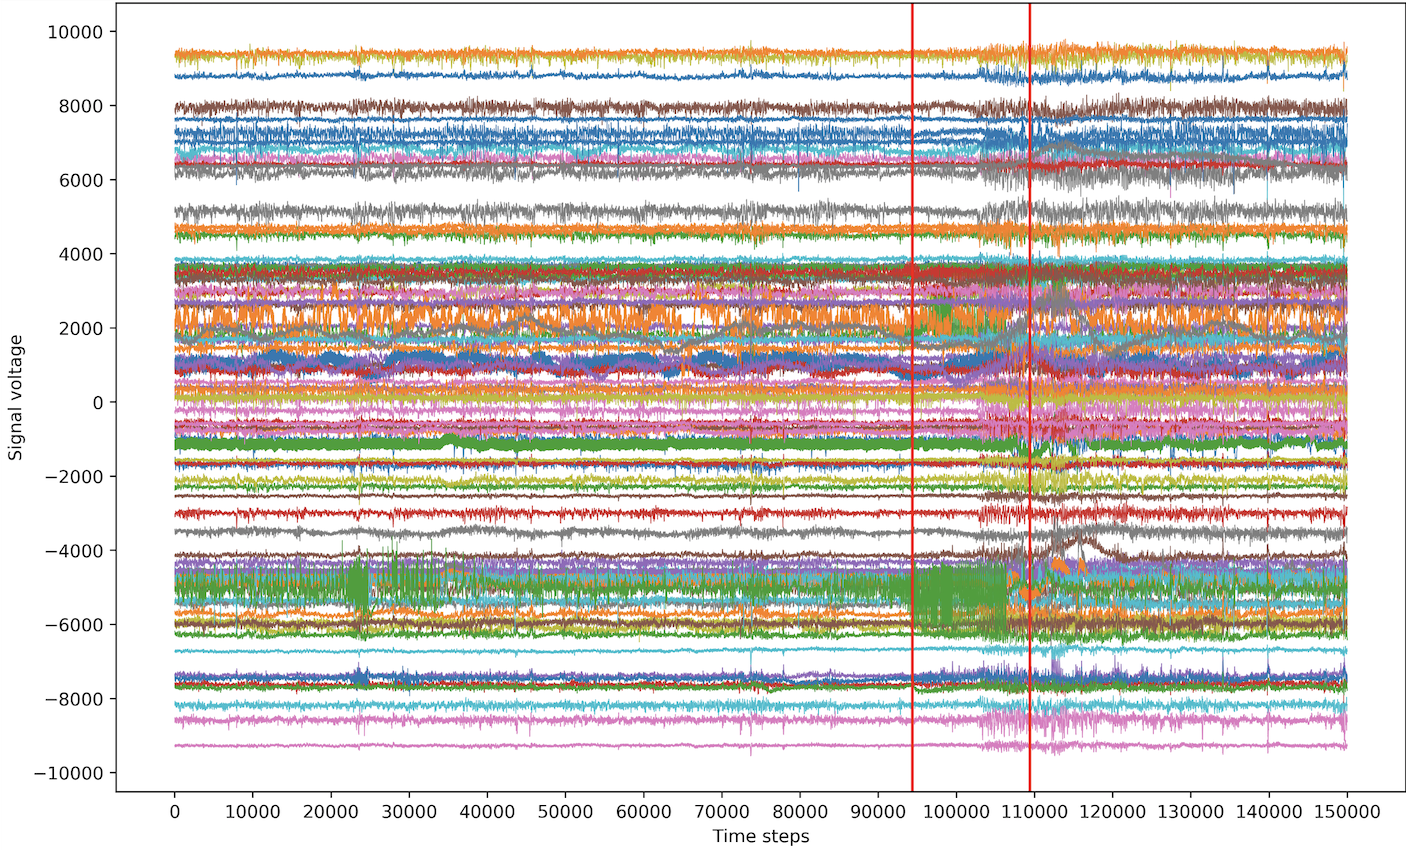
\includegraphics[width=1\textwidth]{plot_seizure1_lowquality}
        \caption{First epileptic seizure}
        \label{fig:plot_seizure1}
	\end{subfigure}
	~
	\begin{subfigure}[t]{0.7\textwidth}
		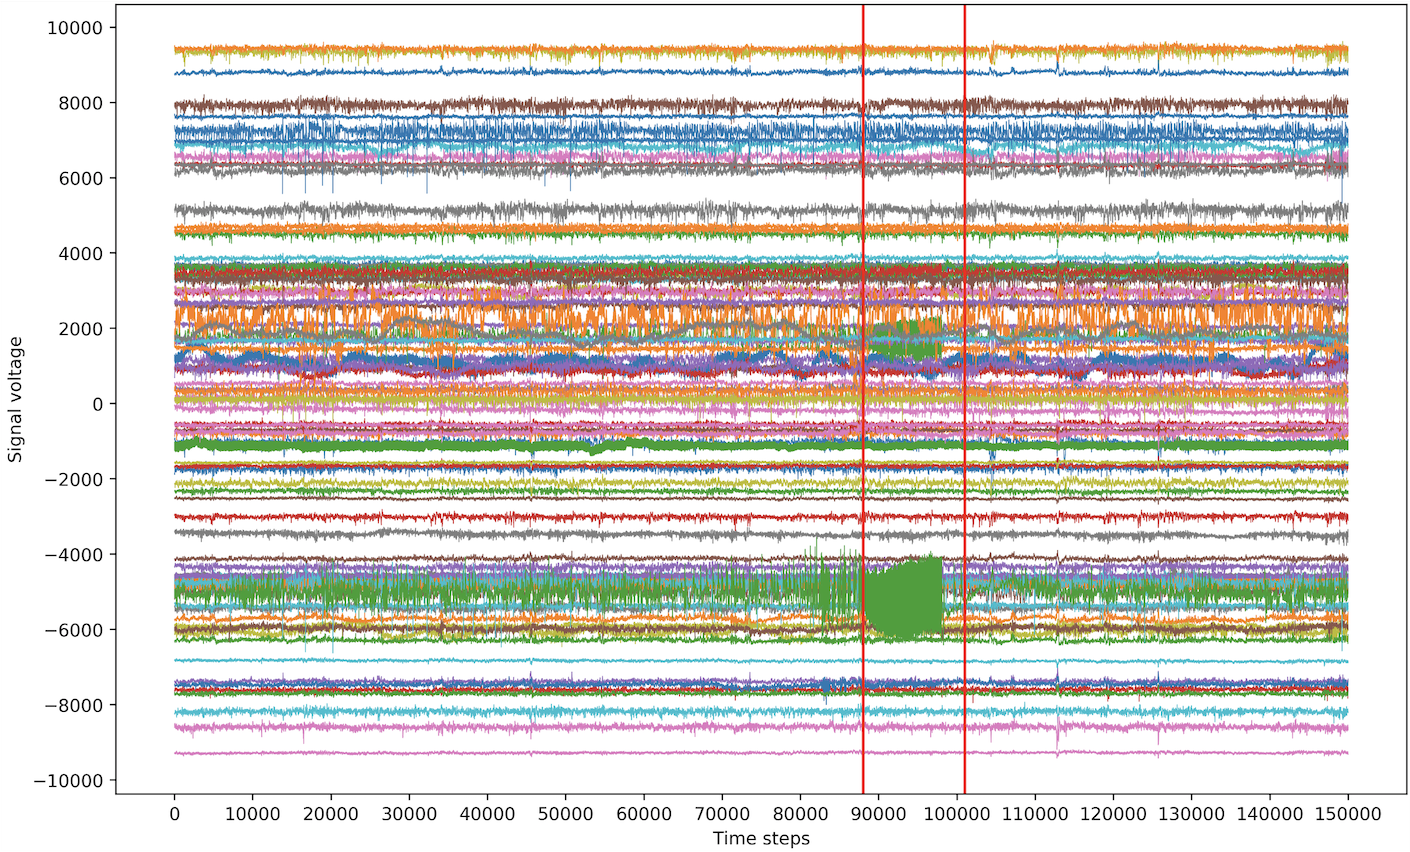
\includegraphics[width=1\textwidth]{plot_seizure2_lowquality}
        \caption{Second epileptic seizure}
        \label{fig:plot_seizure2}
    \end{subfigure}
    ~
    \begin{subfigure}[t]{0.7\textwidth}
		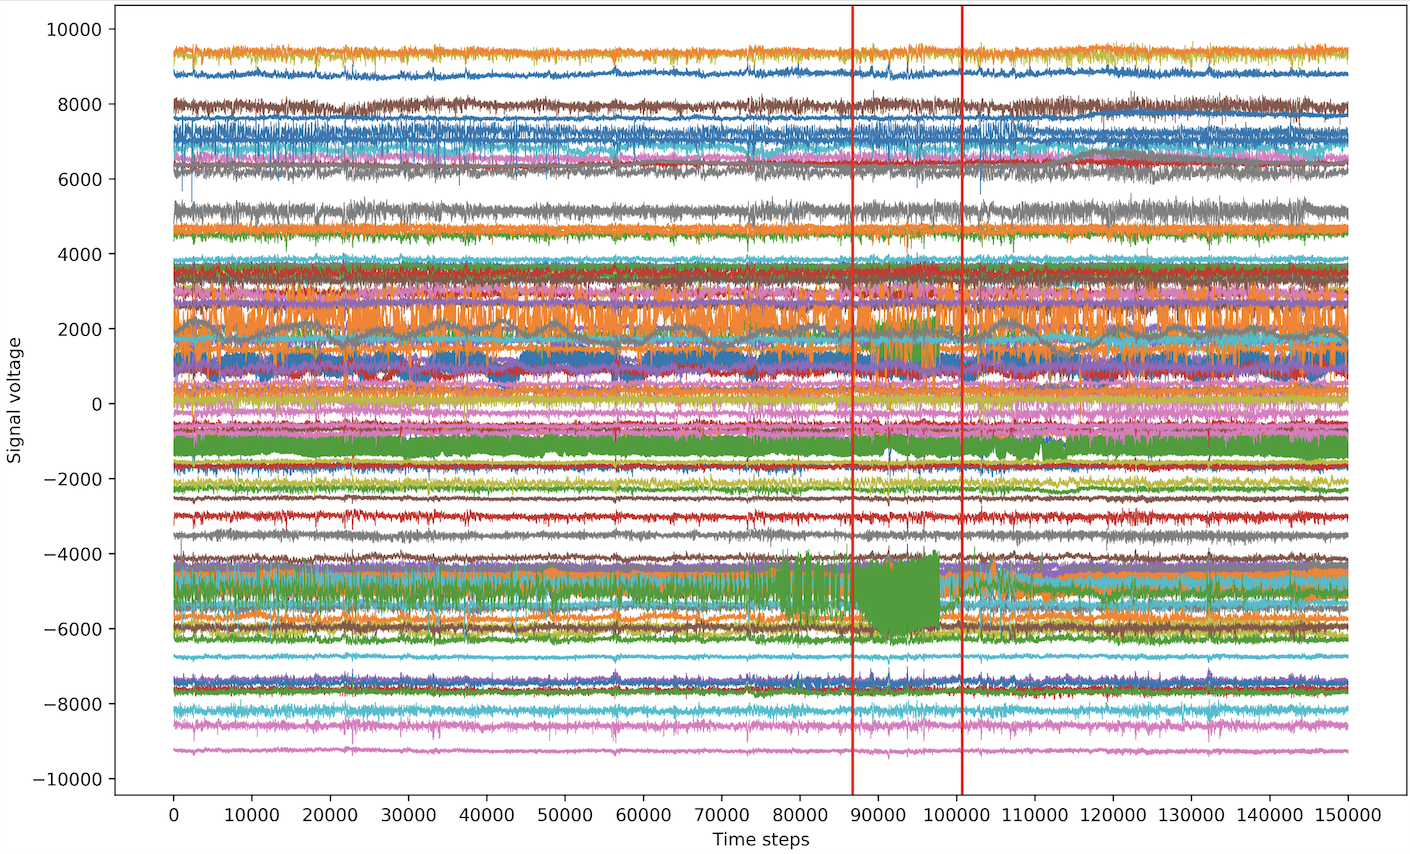
\includegraphics[width=1\textwidth]{plot_seizure3_lowquality}
        \caption{Third epileptic seizure}
        \label{fig:plot_seizure3}
	\end{subfigure}
    \caption{Plots of the \acs{ieeg} around the three epileptic seizures (we suggest to zoom-in the figures in the pdf file). The \acs{ieeg} plots show the voltage values of the 90 channels with respect to time, with y axis in common (hence the time-series overlap). The onset and offset of the seizures are marked by red lines.}
    \label{fig:plot_seizures}
\end{figure}
% \begin{figure}[H]
%     \centering
%     \begin{subfigure}[t]{0.7\textwidth}
% 		\includegraphics[width=1\textwidth]{plot_seizure1}
%         \caption{First epileptic seizure}
%         \label{fig:plot_seizure1}
% 	\end{subfigure}
% 	~
% 	\begin{subfigure}[t]{0.7\textwidth}
% 		\includegraphics[width=1\textwidth]{plot_seizure2}
%         \caption{Second epileptic seizure}
%         \label{fig:plot_seizure2}
%     \end{subfigure}
%     ~
%     \begin{subfigure}[t]{0.7\textwidth}
% 		\includegraphics[width=1\textwidth]{plot_seizure3}
%         \caption{Third epileptic seizure}
%         \label{fig:plot_seizure3}
% 	\end{subfigure}
%     \caption{Plots of the \acs{ieeg} around the three epileptic seizures (we suggest to zoom-in the figures in the pdf file). The \acs{ieeg} plots show the voltage values of the 90 channels with respect to time, with y axis in common (hence the time-series overlap). The onset and offset of the seizures are marked by red lines.}
%     \label{fig:plot_seizures}
% \end{figure}
\newpage

Looking at Figure \ref{fig:plot_seizures}, we are not able to precisely identify the presence of a seizure in the \acs{ieeg}, since the task of seizure detection is too complex for an untrained eye and the dynamic of the electrodes signals does not seem to undergo a big change in correspondence of the beginning of a seizure. In any case, we expect the seizure to be represented not directly by the dynamic of the signals, but by the non-linear relations between the electrodes signal's dynamic through time.

The amount of positive time steps, that are the ones inside the seizure portions, corresponds only to the $9.3$\% of the data, with the remaining $90.7$\% of data being negative time steps; therefore we are dealing with very unbalanced data (see Figure \ref{fig:hist_classes}). The extreme unbalance of the data, together with the severe restriction in the amount of data, make this dataset very difficult to work with, but at the same time very similar to a real-world scenario.
\begin{figure}[htbp]
    \centering
    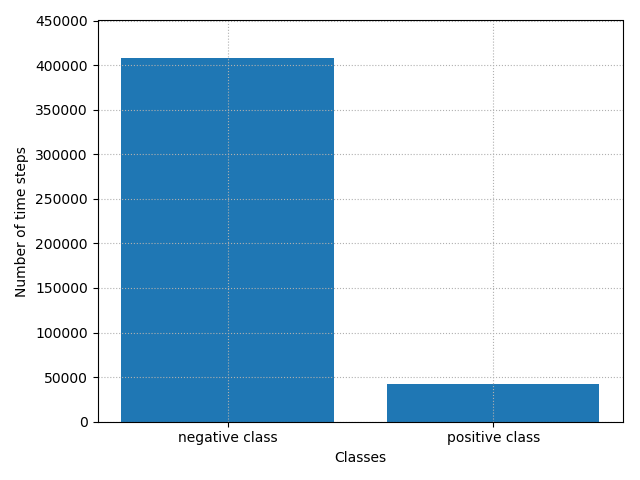
\includegraphics[width=0.6\textwidth]{hist_classes}
    \caption{Histogram of the number of time step for each class}
    \label{fig:hist_classes}
\end{figure}

In order to have an idea of the linear relation between electrodes values, we computed the Pearson correlation coefficient on two sequences of 5 seconds each, one of negative time steps and the other of positive time steps. In Figure \ref{fig:corr_heatmaps} we show the related correlation heatmaps. As you can see from the figures, the correlation heatmap related to the positive time steps reveals a higher linear relation between electrodes values if compared to the correlation heatmap related to the negative time steps. The correlation heatmaps, however, present only the linear relations between data, while we believe that there are hidden non-linear relation between electrodes signal through time which could be crucial for the identification of epileptic seizures.

\begin{figure}[htbp]
    \centering
    \begin{subfigure}[t]{0.49\textwidth}
		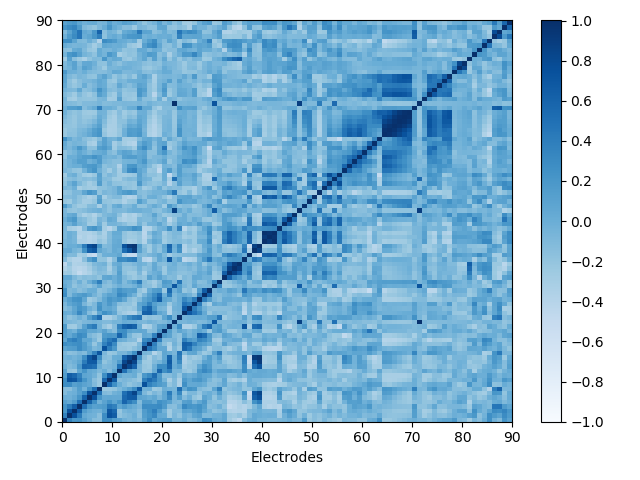
\includegraphics[width=1\textwidth]{corr_nonseizure}
        \caption{Correlation heatmap of 5 seconds of negative time steps}
        \label{fig:corr_nonseizure}
	\end{subfigure}%
	~
	\begin{subfigure}[t]{0.49\textwidth}
		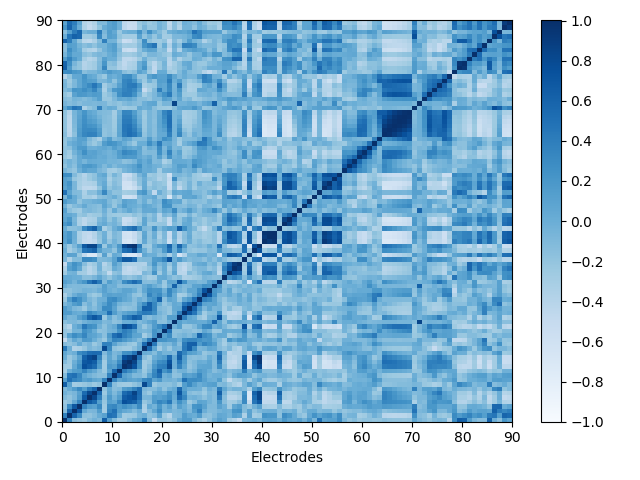
\includegraphics[width=1\textwidth]{corr_seizure}
        \caption{Correlation heatmap of 5 seconds of positive time steps}
        \label{fig:corr_seizure}
    \end{subfigure}
    \caption{Comparison of correlation heatmaps related to negative and positive time steps}
    \label{fig:corr_heatmaps}
\end{figure}

To have another confirmation of the presence of some linear relation between electrodes signals, we computed the standard deviation of the oscillation of each electrode, but this time we computed the mean of the standard deviation both over the negative time steps and over the positive ones. The average standard deviation of the oscillation of each electrode over the negative time steps was around 80 \acs{uv}, while the one over the positive time steps was around 93 \acs{uv}. This shows that, during an epileptic seizure, electrodes signals tends to have wider fluctuation margins, but the difference from the standard fluctuation margins does not seems to be enough to identify a seizure.

%----------------------------------------------------------------
% Data preprocessing
%----------------------------------------------------------------

\section{Data preprocessing} \label{sec: data_preprocessing}
\paragraph{} Once we familiarized with the dataset, we preprocessed it in order to shape it to the right form to be the input of machine learning and deep learning models for the different prediction tasks. As already mentioned in Section \ref{sec: data_analysis_preprocessing}, we divided the data in a training set and a test set, using two seizures' data in the training set and the remaining seizure's data in the test set. The data was prepared to be used by different models for the three prediction tasks described in Section \ref{sec: problem_definition}. Depending on the model and on the task at hand, a sample could represent a time step, a sequence of samples or a sequence of graphs.

\subsection{Time steps as samples}
\paragraph{} This data configuration has been used only for the problem case of detection on a time step; therefore it as been used as input to random forest, gradient boosting, \acs{svm} and dense neural network. In order to prepare data with each time step representing a sample, no additional operations where required, since the dataset was already provided as a big sequence of time step - target couples. Since \acsp{svm} and neural networks are sensible to the scaling of the data, in those cases a \texttt{StandardScaler} from scikit-learn library has been added. The \texttt{StandardScaler} standardize the features of a sample such that the data distribution will have a mean value equal to 0 and a standard deviation value equal to 1. The standardization is computed as:
\begin{align}
    z=\frac{x-\mu}{\sigma} \qquad\qquad \text{with}\qquad &\mu=\frac{1}{N} \sum_{i=1}^{N}\left(x_{i}\right)\\
                                        \text{and}\qquad &\sigma=\sqrt{\frac{1}{N} \sum_{i=1}^{N}\left(x_{i}-\mu\right)^{2}}
\end{align}
where $z$ is the standardized version of $x$, $\mu$ is the mean of $x$ and $\sigma$ is the standard deviation of $x$.

\subsection{Sequences of time steps as samples}
\paragraph{} This data configuration has been used for the problem cases both of detection on a sequence and of prediction on a sequence. The sequences of time steps generated have been the input to standard convolutional and 
\acs{lstm} neural networks. In order to prepare data with each sequence of time steps representing a sample, the dataset has been converted in a set of sequences with a single target associated to each sequence. To do that, we considered different hyperparameters.

The \texttt{'look back'} parameter indicates the number of time steps contained in each sequence; in other words it represents the amount of time steps at which the model can look at in order to predict a target.

The \texttt{'target steps ahead'} parameter determines how far in the future we want the target time step of a sequence to be, starting from the position of the last time step of the sequence. This means that if we consider the \texttt{'target steps ahead'} to be zero, the model will use the sequence's features to predict the target associated with the last time step of the sequence, that corresponds to the problem case of detection on a sequence. Alternatively, if we consider the \texttt{'target steps ahead'} to be higher than zero, the model will use the sequence's features to predict the target associated with a time step outside the sequence and in the future, that corresponds to the problem case of prediction on a sequence.

The \texttt{'stride'} parameter represents the size of the distance between the beginning time step of two consecutive sequences. For instance, if we use a \texttt{'stride'} equal to 1, the sequences will begin time steps at indices $i_0, i_1, i_2, i_3, ...$, while if we use a \texttt{'stride'} equal to 3, the sequences will begin with time steps at indices $i_0, i_3, i_6, i_9, ...$.

The \texttt{'subsampling factor'} parameter allows to downsample the number of sequences by indicating the factor of negative samples to keep with respect to the positive ones. This means that if, for example, we consider the \texttt{'subsampling factor'} to be five, for each positive sample we will keep only five negative samples. This is useful in order to decrease the unbalance in the data. The \texttt{'subsample'} parameter controls whether to apply the downsampling effect or not.

In order to generate the sequences of time steps, we considered one time step index at a time, we took the previous \texttt{'look back'} time steps to create the sequence and we looked \texttt{'target steps ahead'} time steps ahead to identify the target to assign to the sequence. After that, we considered the next time step index, which was \texttt{'stride'} time steps after the current one, and repeated the process. After having created all the sequences, we discarded some random negative sequences in order to respect the proportion between positive and negative samples given by the \texttt{'subsampling factor'}.

In order to create this data configuration, we preprocessed the data by first applying a \texttt{StandardScaler}, like in the previous case, and then generating the sequences both for the training set and the test set, using the same hyperparameters for both of them. The only difference was the fact that we did not use subsampling for the test set, since during the testing of the model we do not need to compensate the unbalance of the dataset.

\subsection{Sequences of graphs as samples}
\paragraph{} This data configuration has been used for the problem cases both of detection on a sequence and of prediction on a sequence. The sequences of graphs generated has been the input to graph-based convolutional and 
\acs{lstm} neural networks. In order to prepare data with each sequence of graphs representing a sample, the first part of the preprocessing process has been the same as for the sequences of time steps: we first applied a \texttt{StandardScaler} and then generated the sequences both for the training set and the test set, without subsampling the test set. After that, an additional operation was required, that is the transformation of the sequences of time steps into sequences of graphs.

As already mentioned in Section \ref{sec: fc_graphs}, the sequences of time steps can be transformed into sequences of graphs by computing the functional connectivity between electrodes and generating a corresponding graph for each time window. To do that, we considered one sequence at a time and we divided it into a fixed number of time windows, each one containing the same number of time steps. For each time window, we built a graph having one node for each electrode and we used the correlation values between electrodes signal in that time window as edge attribute. The number of edges was limited by keeping only the edges with most significative correlation values. Through this process, we generated a graph for each time window in the sequence, therefore the sequence of time steps was transformed in a sequence of graphs. The target remained the same as for sequences of time steps.

This procedure has been implemented with the function \texttt{get\_fc} from \texttt{Spektral} library, which does exactly what just described: it takes a sequence of time steps as input, it divides it in time windows, it computes the functional connectivity between electrodes inside each time window and it outputs the resulting sequence of graphs. For the creation of the sequences of graphs, we considered some additional parameters: the \texttt{'samples per graph'} parameter determines the dimension of the time windows to divide the sequence and the \texttt{'percentiles'} parameter controls which edges in the graphs will be removed. To be more specific, to decide the values for \texttt{'percentiles'}, we choose two numbers between 0 and 100 and we remove from each graph the links with correlation value between the two percentiles.

\subsection{Cross-validation}
\paragraph{} In order to have representative results, we performed k-fold cross validation for all the models and the tasks. Cross validation is a useful technique to evaluate machine learning models, especially when there is a limited amount of data at disposal and we cannot rely on the validation set. In order to perform k-folds cross validation, the dataset is divided into $k$ subsets (folds), of which $k-1$ folds are used as training set and the remaining fold as test set. The training-testing process is performed $k$ times, so that each fold is used as test set one time and it is included in the training set all the other times. To perform cross validation with our data, we divided the dataset into three subsets (3-folds cross validation), each one containing one of the three seizures, and we prepared the three corresponding training and test sets, each time using two folds as training set and the remaining fold as test set.

%----------------------------------------------------------------
% Experiments
%----------------------------------------------------------------

\section{Experiments} \label{sec: experiments}
\paragraph{} As already mentioned in Section \ref{sec: models_application}, a big amount of experiments have been conducted in order to apply the chosen machine learning and deep learning models to the three cases of the problem of epileptic seizures prediction. These experiments helped to identify the best-performing configuration for each model on the task at hand. This section will present the models architectures and parameters that have been tested and the best configuration that has been selected for each model, which generated the results described in section \ref{sec: results}. The best configuration was chosen by looking for the best trade-off between the evaluation metrics over the 3-fold cross-validation.

\subsection{Support Vector Machine experiments}
\paragraph{} The \acs{svm} model has been tested on the problem of detection based on a single time step. We did not make a lot of experiments using \acs{svm}, since the poor results immediately suggested that this machine learning algorithm is too weak to handle the complexity of the seizure prediction task.

In order to test the \acs{svm} model, we used the \texttt{svm.SVC} implementation from scikit-learn library. We kept all the parameters to the default values, except for the \texttt{gamma} and \texttt{class\_weight} parameters. The \acs{svm} has been tested with a penalty parameter $C=1$ and using a Gaussian radial basis function (\acs{rbf}) kernel. The \texttt{gamma} value was set to \texttt{'scale'}, that corresponds to $\frac{1}{F \cdot var(X)}$, where $F$ is the number of features and $var(X)$ is the variance of the input features. We tested both a balanced and an unbalanced version of the \acs{svm} by setting the \texttt{class\_weight} parameter to \texttt{'balanced'} or leaving it to \texttt{None} and we obtained slightly better results using the balanced configuration of the model. Table \ref{tab:svm_param} presents the parameters of the \acs{svm} model that performed better.
\begin{table}[htbp]
    \centering
    \begin{tabular}{ll}
        \hline
        \textbf{Parameter}  & \textbf{Value} \\\hline
        C                   & 1 \\
        kernel              & \texttt{'rbf'} \\
        gamma               & \texttt{'scale'} \\
        balanced            & \texttt{True} \\\hline
    \end{tabular}
    \caption{Parameters of best-performing \acs{svm} model}
    \label{tab:svm_param}
\end{table}

\subsection{Random forest experiments}
\paragraph{} The random forest model has been tested on the problem of detection based on a single time step.

In order to test the random forest model, we used the \texttt{ensemble.RandomForest}-\texttt{Classifier} implementation from scikit-learn library. We kept all the parameters to the default values, except for the \texttt{n\_estimators}, the \texttt{max\_depth} and \texttt{class\_weight} parameters. The \texttt{criterion} parameter to measure the quality of a split was set to \texttt{'gini'}, which corresponds to the Gini impurity function. We tried several values for \texttt{n\_estimators}, which is the number of trees in the forest, and for \texttt{max\_depth}, which is the maximum depth of the tree, in order to find the best balance between the two. We tested both a balanced and an unbalanced version of the random forest classifier by setting the \texttt{class\_weight} parameter to \texttt{'balanced'} or leaving it to \texttt{None} and there was no resulting difference between the two configurations. Table \ref{tab:randomforest_param} presents the parameters of the random forest model that performed better.
\begin{table}[htbp]
    \centering
    \begin{tabular}{ll}
        \hline
        \textbf{Parameter}  & \textbf{Value} \\\hline
        n\_estimators       & 20 \\
        max\_depth          & 8 \\
        criterion           & \texttt{'gini'} \\
        balanced            & \texttt{True/False} \\\hline
    \end{tabular}
    \caption{Parameters of best-performing random forest model}
    \label{tab:randomforest_param}
\end{table}

\subsection{Gradient boosting experiments}
\paragraph{} The gradient boosting model has been tested on the problem of detection based on a single time step.

In order to test the gradient boosting model, we used the \texttt{XGBClassifier} implementation from xgboost library. We kept all the parameters to the default values, except for the \texttt{n\_estimators}, the \texttt{max\_depth} and \texttt{scale\_pos\_weight} parameters. The \texttt{booster} parameter was set to \texttt{'gbtree'} in order to use a tree-based booster. As for the random forest model, we tried different values for \texttt{n\_estimators} and for \texttt{max\_depth} in order to find the best balance between the two. We tested both a balanced and an unbalanced version of the random forest classifier by setting the \texttt{scale\_pos\_weight} parameter to $\frac{\texttt{num\_negative}}{\texttt{num\_positive}}$, which are respectively the number of negative and positive samples, or by leaving it to \texttt{None} and there was no resulting difference between the two configurations. Table \ref{tab:gradientboosting_param} presents the parameters of the gradient boosting model that performed better.
\begin{table}[htbp]
    \centering
    \begin{tabular}{ll}
        \hline
        \textbf{Parameter}  & \textbf{Value} \\\hline
        n\_estimators       & 20 \\
        max\_depth          & 4 \\
        booster             & \texttt{'gbtree'} \\
        balanced            & \texttt{True/False} \\\hline
    \end{tabular}
    \caption{Parameters of best-performing gradient boosting model}
    \label{tab:gradientboosting_param}
\end{table}

\subsection{Dense neural network experiments}
\paragraph{} The dense neural network model has been tested on the problem of detection based on a single time step.

In order to test the \acs{fcnn} model, we used the \texttt{Dense} and \texttt{Dropout} layers implementation from Tensorflow's Keras library. We investigated several configurations of the model by trying different values for the number of dense layers (\texttt{depth\_dense}), the number of units in each layer (\texttt{units}), the activation function to use (\texttt{activation}), the amount of $\ell_2$ regularization to apply to the kernel (\texttt{kernel\_regularizer}) and the dropout rate to apply between the dense layers (\texttt{dropout}). During the training of the model, we used the \texttt{class\_weight} parameter to compensate the unbalance of the dataset.

The model configuration which obtained the best results is composed by three fully-connected layers, with a dropout layer after each one of them. The first two dense layer have 512 units, while the third one has 256 units, and they all use the \acs{relu} activation function and the $\ell_2$ kernel regularization. After the three dense layers, there is a fourth dense layer with only 1 unit and a sigmoid activation function in order to output the prediction. Table \ref{tab:dense_param} presents the parameters of the dense neural network model that performed better.
\begin{table}[htbp]
    \centering
    \begin{tabular}{ll}
        \hline
        \textbf{Parameter}  & \textbf{Value} \\\hline
        epochs              & 20 \\
        batch\_size         & 32 \\
        depth\_dense        & 4 \\
        units               & 512 / 256 \\
        activation          & \texttt{'relu'} \\
        kernel\_regularizer & \texttt{l2(5e-2)} \\
        dropout             & 0.4 \\
        class\_weight       & \{0: $\frac{N}{\texttt{num\_negative}}$, 1: $\frac{N}{\texttt{num\_positive}}$\} \\\hline
    \end{tabular}
    \caption{Parameters of best-performing dense neural network model}
    \label{tab:dense_param}
\end{table}

\subsection{Convolutional neural network experiments}
\paragraph{} The convolutional neural network model has been tested on the problems of detection and prediction based on a sequence of time steps.

In order to test the \acs{cnn} model, we used the \texttt{Conv1D}, \texttt{MaxPooling1D}, \texttt{Flatten}, \texttt{Dense}, \texttt{Dropout} and \texttt{BatchNormalization} layers implementation from Tensorflow's Keras library. We investigated several configurations of the model by first trying different values for the main parameters of the neural network: the number of convolutional layers (\texttt{depth\_conv}), the number of dense layers for the prediction (\texttt{depth\_dense}), the number of output filters in the convolution (\texttt{filters}), the length of the convolution window (\texttt{kernel\_size}), the activation function to use (\texttt{activation}), the amount of $\ell_2$ regularization to apply to the kernel (\texttt{kernel\_regularizer}), the presence of batch normalization (\texttt{batch\_norm}) and the dropout rate (\texttt{dropout}) to apply between the dense layers. During the training of the model, we used the \texttt{class\_weight} parameter to compensate the unbalance of the dataset.

After the first promising results, we tried to improve the performances of the model by using dilated convolution. Using this technique, the filter is "dilated" before its application, meaning that its size is expanded by filling the empty positions with zeros. This means that the filter's dimensions are not altered, but its weights are matched to not-adjacent instances in the input matrix. The distance between the instances is determined by the dilation rate $D$. Figure \ref{fig:nn_conv_dilated} shows an example of a $3 \times 3$ dilated convolution with $D=2$.
\begin{figure}[htbp]
    \centering
    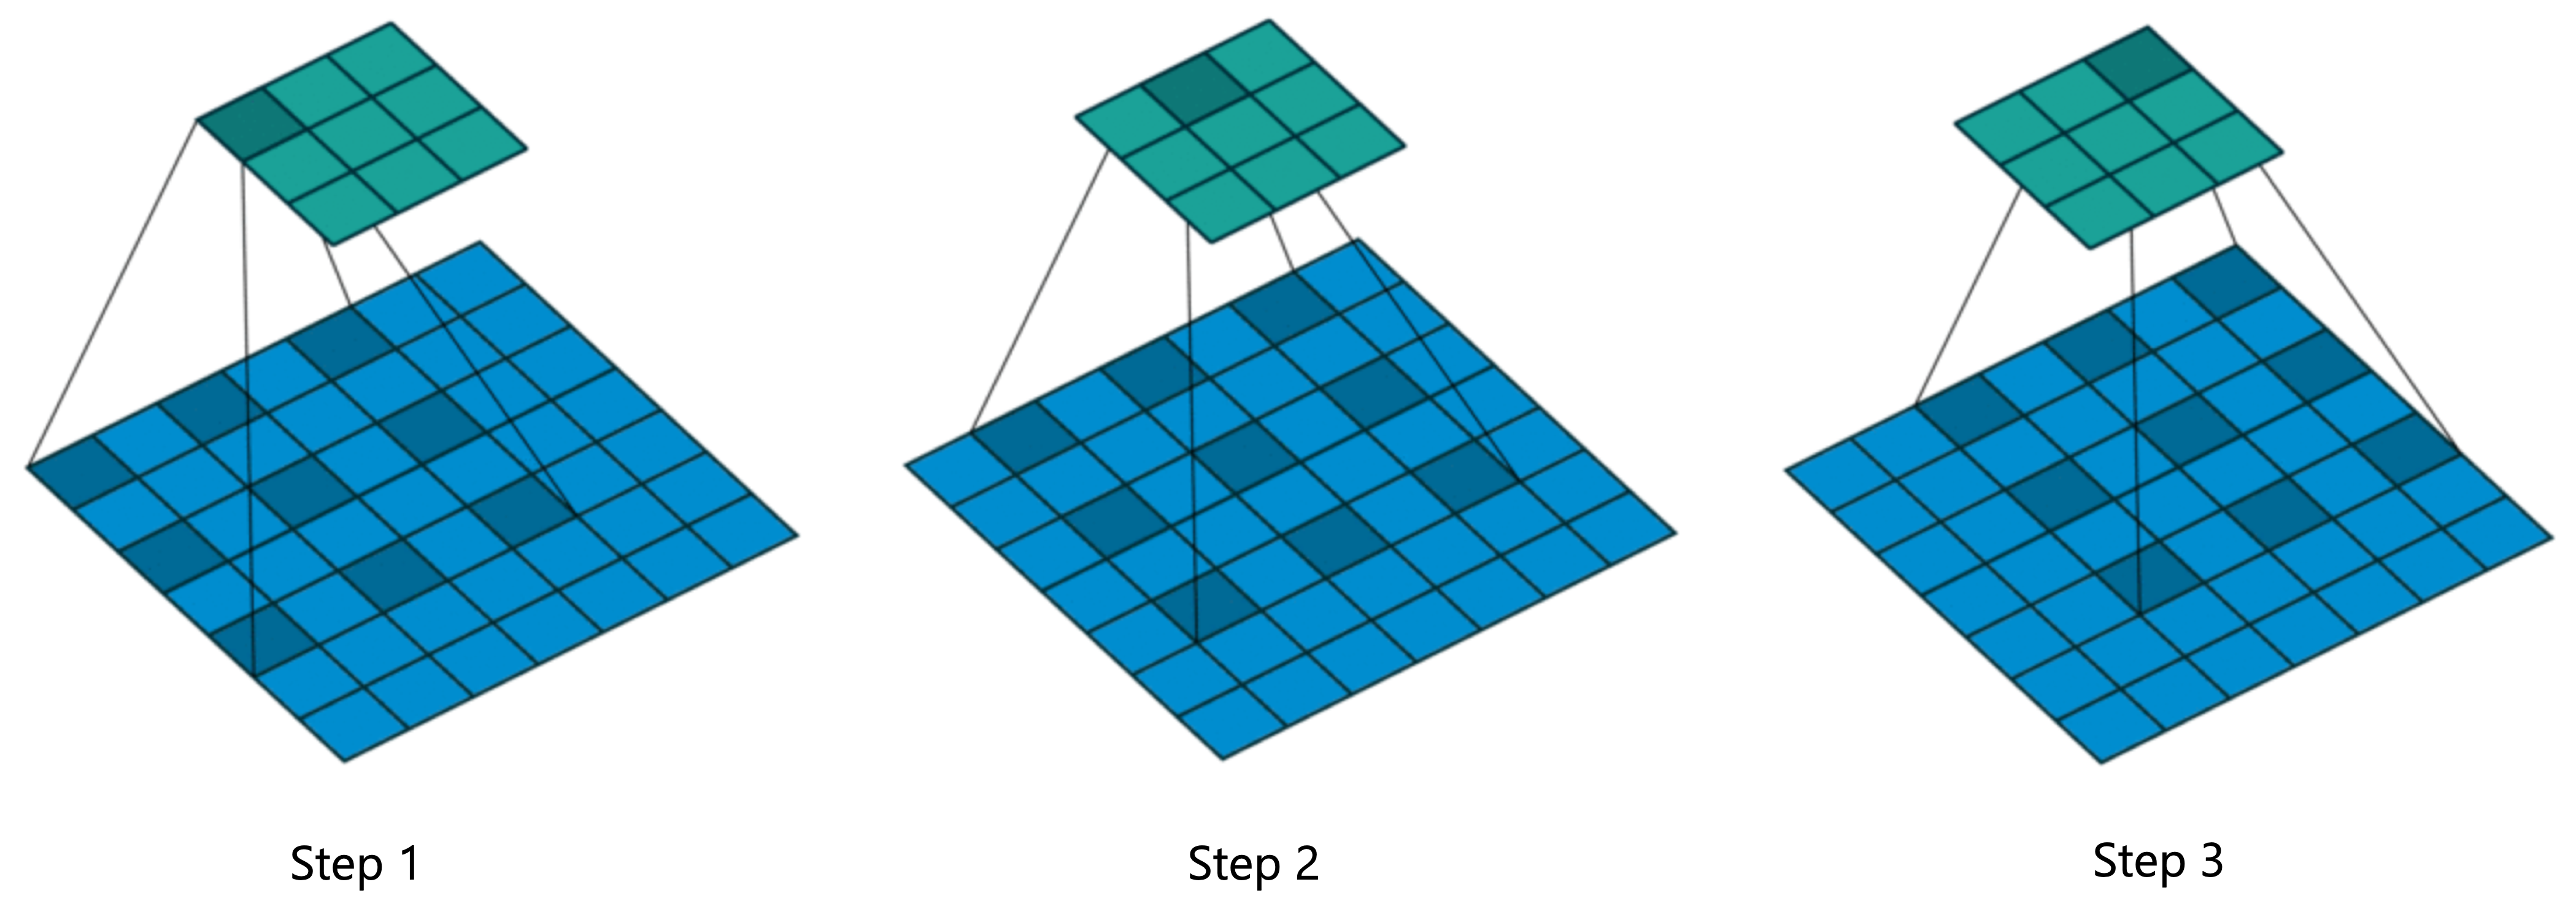
\includegraphics[width=0.8\textwidth]{nn_conv_dilated}
    \caption{Sequence of receptive fields with dilation rate equal to 2 (from \textit{Medium - Towards Data Science})}
    \label{fig:nn_conv_dilated}
\end{figure}

In order to test the model with dilated convolution, we added the dilation rate (\texttt{dilation\_rate}) parameter to the hyperparameters search and we set the padding (\texttt{padding}) to \texttt{'causal'}. In this way, we are limiting the filter at time step $t$ so that it can only see inputs that are no later than $t$. This is done by padding the layer's input with zeros in the front. In order to generalize better, we also added a max-pooling layer after each convolutional layer (\texttt{pooling}).

The \acs{cnn} model was tested both on detection and prediction problems and on different values of \texttt{look\_back} and \texttt{target\_steps\_ahead} for the creation of the input sequences, so we identified different "best" configurations. In general, the architecture that worked better is composed by two or three convolutional layers, each one followed by a max-pooling layer, and by two final fully-connected layers (the first one having 256 units), with a batch normalization layer and a dropout layer between the two. The convolutional layers use 64 filters, except for the last one which uses 32 filters; the kernel size is set to 3 and the convolution is made with a dilation rate equal to 3. All the layers use the \acs{relu} activation function and the $\ell_2$ kernel regularization, except for the last dense layer, which has only 1 unit and which uses a sigmoid activation function in order to output the prediction. 

Table \ref{tab:conv_param} presents the parameters of the dense neural network model that performed better. The best-performing parameters are the same both for the detection and prediction problems, with the only difference in the number of convolutional layers, which for the prediction task varies between two and three depending on the value of \texttt{target\_steps\_ahead}.
\begin{table}[htbp]
    \centering
    \begin{tabular}{ll}
        \hline
        \textbf{Parameter}  & \textbf{Value} \\\hline
        epochs              & 10 \\
        batch\_size         & 64 \\
        depth\_conv         & 2 \\
        depth\_dense        & 2 \\
        filters             & 64 \\
        kernel\_size        & 3 \\
        activation          & \texttt{'relu'} \\
        batch\_norm         & \texttt{True} \\
        kernel\_regularizer & \texttt{l2(5e-1)} \\
        dropout             & 0.4 \\
        pooling             & \texttt{True} \\
        pool\_size          & 2 \\
        padding             & \texttt{'causal'} \\
        dilation\_rate      & 3 \\
        class\_weight       & \{0: $\frac{N}{\texttt{num\_negative}}$, 1: $\frac{N}{\texttt{num\_positive}}$\} \\\hline
    \end{tabular}
    \caption{Parameters of best-performing convolutional neural network model}
    \label{tab:conv_param}
\end{table}

\subsection{\acs{lstm} neural network experiments}
\paragraph{} The \acs{lstm} neural network model has been tested on the problems of detection and prediction based on a sequence of time steps.

In order to test the \acs{lstm} model, we used the \texttt{LSTM}, \texttt{Dense}, \texttt{Dropout} and \texttt{Batch}-\texttt{Normalization} layers implementation from Tensorflow's Keras library. We investigated several configurations of the model by trying different values for the number of \acs{lstm} layers (\texttt{depth\_lstm}), the number of dense layers (\texttt{depth\_dense}), the number of units in each \acs{lstm} layer (\texttt{units\_lstm}), the activation function to use (\texttt{activation}), the amount of $\ell_2$ regularization to apply to the kernel (\texttt{kernel\_regularizer}), the presence of batch normalization (\texttt{batch\_norm}) and the dropout rate (\texttt{dropout}) to apply between the layers. During the training of the model, we used the \texttt{class\_weight} parameter to compensate the unbalance of the dataset.

The \acs{lstm} model was tested both on detection and prediction problems and on different values of \texttt{look\_back} and \texttt{target\_steps\_ahead} for the creation of the input sequences; however we identified a single configuration that obtained the best results in all the tasks. The architecture that worked better is composed by one \acs{lstm} layer followed by two fully-connected layers (the first one having 256 units), with a batch normalization layer and a dropout layer between the three layers. The \acs{lstm} layer uses 256 units and all the layers use the \acs{relu} activation function and the $\ell_2$ kernel regularization, except for the last dense layer, which has only 1 unit and which uses a sigmoid activation function in order to output the prediction. Table \ref{tab:lstm_param} presents the parameters of the \acs{lstm} neural network model that performed better.
\begin{table}[htbp]
    \centering
    \begin{tabular}{ll}
        \hline
        \textbf{Parameter}  & \textbf{Value} \\\hline
        epochs              & 15 \\
        batch\_size         & 64 \\
        depth\_lstm         & 1 \\
        depth\_dense        & 2 \\
        units\_lstm         & 256 \\
        activation          & \texttt{'relu'} \\
        batch\_norm         & \texttt{True} \\
        kernel\_regularizer & \texttt{l2(5e-1)} \\
        dropout             & 0.4 \\
        class\_weight       & \{0: $\frac{N}{\texttt{num\_negative}}$, 1: $\frac{N}{\texttt{num\_positive}}$\} \\\hline
    \end{tabular}
    \caption{Parameters of best-performing \acs{lstm} neural network model}
    \label{tab:lstm_param}
\end{table}

\subsection{Graph-based convolutional neural network experiments}
\paragraph{} The graph-based convolutional neural network model has been tested on the problems of detection and prediction based on a sequence of graphs.

The graph-based \acs{cnn} model has been implemented and tested in the same way as the standard \acs{cnn} model, conducting hyperparameters search on the same parameters and using a similar architecture. The main difference is the addition of an edge-conditioned convolutional layer (\acs{ecc}), followed by a global average-pooling, just before the use of the standard \acs{cnn}. This is necessary in order to convert the input graphs into expressive features that can be processed by the standard \acs{cnn}. In addition to the \acs{cnn} parameters, we tested different values also for the number of output filters in the edge-conditioned convolution (\texttt{g\_filters}).

The graph-based \acs{cnn} model was tested both on detection and prediction problems and on different values of \texttt{look\_back} and \texttt{target\_steps\_ahead} for the creation of the input sequences; however we identified a single configuration that obtained the best results in all the tasks, even though the graph-based \acs{cnn} performance in general were poor. As already mentioned, the configuration is the same as for the standard \acs{cnn} with a \acs{ecc} and a global average-pooling layers added at the beginning. Table \ref{tab:gconv_param} presents the parameters of the graph-based convolutional neural network model that performed better.
\begin{table}[htbp]
    \centering
    \begin{tabular}{ll}
        \hline
        \textbf{Parameter}  & \textbf{Value} \\\hline
        epochs              & 200 \\
        batch\_size         & 32 \\
        depth\_conv         & 3 \\
        depth\_dense        & 2 \\
        filters             & 64 \\
        kernel\_size        & 3 \\
        g\_filters          & 32 \\
        activation          & \texttt{'relu'} \\
        batch\_norm         & \texttt{True} \\
        kernel\_regularizer & \texttt{l2(5e-3)} \\
        dropout             & 0.4 \\
        pooling             & \texttt{True} \\
        pool\_size          & 2 \\
        padding             & \texttt{'causal'} \\
        dilation\_rate      & 3 \\
        class\_weight       & \{0: $\frac{N}{\texttt{num\_negative}}$, 1: $\frac{N}{\texttt{num\_positive}}$\} \\\hline
    \end{tabular}
    \caption{Parameters of best-performing graph-based convolutional neural network model}
    \label{tab:gconv_param}
\end{table}

\subsection{Graph-based \acs{lstm} neural network experiments}
\paragraph{} The graph-based \acs{lstm} neural network model has been tested on the problems of detection and prediction based on a sequence of graphs.

The graph-based \acs{lstm} model has been implemented and tested in the same way as the standard \acs{lstm} model, conducting hyperparameters search on the same parameters and using a similar architecture. The main difference is the addition of an edge-conditioned convolutional layer (\acs{ecc}), followed by a global average-pooling, just before the use of the standard \acs{lstm}. This is necessary in order to convert the input graphs into expressive features that can be processed by the standard \acs{lstm}. In addition to the \acs{lstm} parameters, we tested different values also for the number of output filters in the edge-conditioned convolution (\texttt{g\_filters}).

The graph-based \acs{lstm} model was tested both on detection and prediction problems and on different values of \texttt{look\_back} and \texttt{target\_steps\_ahead} for the creation of the input sequences; however we identified a single configuration that obtained the best results in all the tasks, even though the graph-based \acs{lstm} performance in general were poor. As already mentioned, the configuration is the same as for the standard \acs{lstm} with a \acs{ecc} and a global average-pooling layers added at the beginning. Table \ref{tab:glstm_param} presents the parameters of the graph-based \acs{lstm} neural network model that performed better.
\begin{table}[htbp]
    \centering
    \begin{tabular}{ll}
        \hline
        \textbf{Parameter}  & \textbf{Value} \\\hline
        epochs              & 150 \\
        batch\_size         & 32 \\
        depth\_lstm         & 1 \\
        depth\_dense        & 2 \\
        units\_lstm         & 256 \\
        g\_filters          & 32 \\
        activation          & \texttt{'relu'} \\
        batch\_norm         & \texttt{True} \\
        kernel\_regularizer & \texttt{l2(5e-3)} \\
        dropout             & 0.4 \\
        class\_weight       & \{0: $\frac{N}{\texttt{num\_negative}}$, 1: $\frac{N}{\texttt{num\_positive}}$\} \\\hline
    \end{tabular}
    \caption{Parameters of best-performing graph-based \acs{lstm} neural network model}
    \label{tab:glstm_param}
\end{table}


%----------------------------------------------------------------
% Results evaluation
%----------------------------------------------------------------

\section{Results evaluation} \label{sec: results}
\paragraph{} For the models evaluation, as already mentioned, four metrics have been used: loss, accuracy, ROC-AUC and recall. In order to evaluate models, we chose as best models the ones that obtained highest recall on test data. For this type of task, recall is very important, as it represents the number of true positive instances ($TP$) over the total number of real positive instances ($TP+FN$); therefore it is able to tell us the probability of correct prediction of a seizure. Being totally focused on the positive class, recall is an evaluation metric particularly suited to unbalanced datasets, since it is not influenced by the number of negative instances. Also ROC-AUC had a crucial role in models evaluation, since we want the classifiers to be consistent and to avoid random prediction. Of course, loss and accuracy have not been ignored, since the models need to correctly classify more than the majority of time steps in order to be significant.

To sum up, in order to choose the preferred configuration for the models, we looked for the best trade-off between the four metrics, slightly prioritizing recall over the others. Following this logic, we selected the best model for each machine learning and deep learning method used on each type of task. This allowed us to make a comparison between the performances of different methods for each task.

As already mentioned before, all the results presented have been computed by taking the mean over the 3-fold cross-validation. When choosing the best models, we payed attention also to the standard deviation of the recall over the three folds, in order to avoid choosing a model that can perform extraordinarily well on a fold and awfully on another fold.


\subsection{Detection on a time step}
\paragraph{} The results of \acs{svm}, random forest, gradient boosting and \acs{fcnn} models on the problem of seizure detection based on a single time step are presented in Table \ref{tab:det_timestep_results} and shown as a barplot in Figure \ref{fig:det_timestep_plots}.
\begin{table}[b]
    \centering
    \begin{tabular}{lllll}
        \hline
                          & \multicolumn{4}{c}{\textbf{Metric}}                                    \\ \cline{2-5} 
        \textbf{Model}    & \textit{loss} & \textit{accuracy} & \textit{ROC-AUC} & \textit{recall} \\ \hline
        SVM               & 2.497         & 75.1 \%           & 0.601            & 0.067           \\
        random forest     & 0.303         & 89.9 \%           & 0.768            & 0.121           \\
        gradient boosting & 0.297         & 89.8 \%           & 0.805            & 0.219           \\
        FCNN              & 0.293         & 90.2 \%           & 0.734            & \textbf{0.248}  \\\hline
    \end{tabular}
    \caption{Results of the models for the problem of detection on a time step}
    \label{tab:det_timestep_results}
\end{table}

\begin{figure}[t]
    \centering
    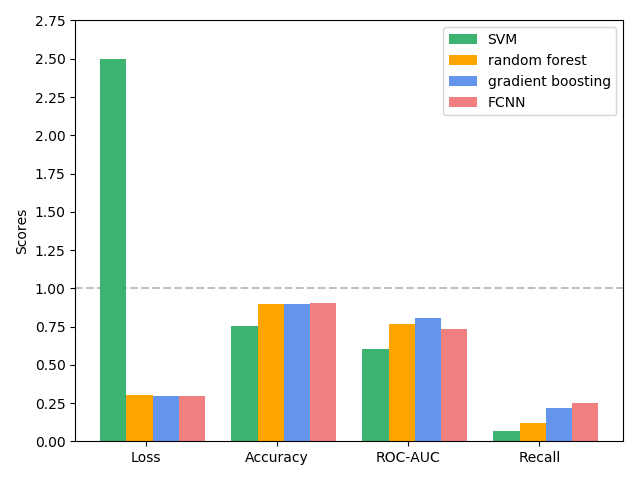
\includegraphics[width=0.7\textwidth]{det_timestep_plots}
    \caption{Barplot of results of the models for the problem of detection on a time step}
    \label{fig:det_timestep_plots}
\end{figure}

As expected, the results on this type of problem were unsatisfactory, since the values of recall do not even come close to the half of positive instances. This means that most of the times the models are not able to correctly detect the presence of a seizure only looking at the features of a single time step. Except for the \acs{svm} model, which obtained the worst results, the other models obtained acceptable performances in predicting general instances, since the accuracy values are around 90 \% and, looking at the ROC-AUC values, the predictions are not random.

The model that performed better on this task was the dense neural network, which was able to correctly detect about a quarter of the positive samples.


\subsection{Detection on a sequence}
\paragraph{} The results of \acs{cnn}, \acs{lstm}, graph-based \acs{cnn} and graph-based \acs{lstm} models on the problem of seizure detection based on a sequence are presented in Table \ref{tab:det_sequence_results} and shown as a barplot in Figure \ref{fig:det_sequence_plots}.
\begin{table}[t]
    \centering
    \begin{tabular}{lllll}
        \hline
                          & \multicolumn{4}{c}{\textbf{Metric}}                                    \\ \cline{2-5} 
        \textbf{Model}    & \textit{loss} & \textit{accuracy} & \textit{ROC-AUC} & \textit{recall} \\ \hline
        CNN               & 0.208         & 94.2 \%           & 0.903            & 0.534           \\
        LSTM              & 0.221         & 95.3 \%           & 0.910            & \textbf{0.580}  \\
        graph-based CNN   & 2.268         & 29.7 \%           & 0.667            & 0.895           \\
        graph-based LSTM  & 1.484         & 69.2 \%           & 0.616            & 0.476           \\\hline
    \end{tabular}
    \caption{Results of the models for the problem of detection on a sequence}
    \label{tab:det_sequence_results}
\end{table}

\begin{figure}[t]
    \centering
    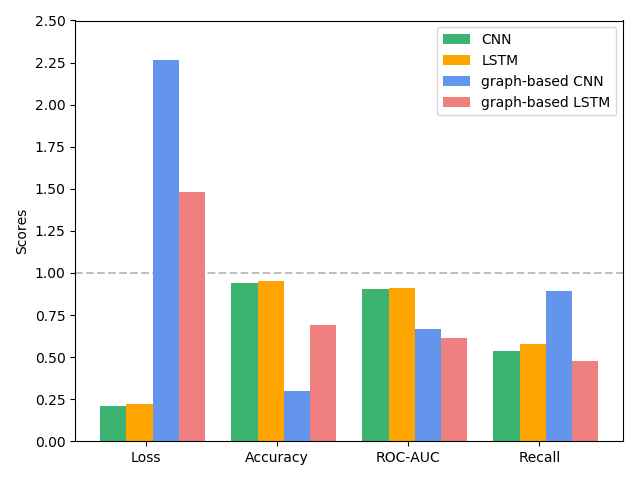
\includegraphics[width=0.7\textwidth]{det_sequence_plots}
    \caption{Barplot of results of the models for the problem of detection on a sequence}
    \label{fig:det_sequence_plots}
\end{figure}

For this type of task, tested different values of \texttt{'look back'} and chose the one that worked better for each model: the CNN model looked at sequences of 100 time steps each; the LSTM model looked at sequences of 200 time steps each; both the graph-based models looked at sequences of 5000 time steps each, corresponding to 10 graphs, each one representing a window of 500 time steps.

The standard \acs{cnn} and \acs{lstm} models achieved acceptable performances, being able to correctly detect more than half of the positive samples. They obtained similar results, but the \acs{lstm} was the model that performed better, since it was able to obtain an higher recall with respect to the \acs{cnn} model. On the other hand, the graph-based models performed very poorly, reaching high loss values, and their prediction where not so far from random predictions. The high recall obtained by the graph-based \acs{cnn} model could be misleading, but the values of the other metrics suggest that it is due to the fact that the model predicts 1 most of the times, without really being able to detect a seizure.


\subsection{Prediction on a sequence}
\paragraph{} For this type of task, after several experiments, we came to the conclusion that the models were not able to correctly predict targets more than 2000 time steps (4 seconds) forward. Passed that threshold, their performances started to rapidly degenerate. For this reason, we chose three \texttt{'target steps ahead'} values as reference for the models evaluation: 500 time steps (1 second), 1000 time steps (2 seconds) and 2000 time steps (4 seconds) forward. The results of \acs{cnn}, \acs{lstm}, graph-based \acs{cnn} and graph-based \acs{lstm} models on the problem of seizure prediction based on a sequence are presented in different tables and barplots based on the value of \texttt{'target steps ahead'}.

Table \ref{tab:pred_sequence500_results} and the barplot in Figure \ref{fig:pred_sequence500_plots} show the results for the prediction of a target 500 time steps (1 second) forward with respect to the associated sequence.
\begin{table}[htbp]
    \centering
    \begin{tabular}{lllll}
        \hline
                          & \multicolumn{4}{c}{\textbf{Metric}}                                    \\ \cline{2-5} 
        \textbf{Model}    & \textit{loss} & \textit{accuracy} & \textit{ROC-AUC} & \textit{recall} \\ \hline
        CNN               & 0.340         & 89.2 \%           & 0.946            & 0.634           \\
        LSTM              & 0.293         & 92.2 \%           & 0.922            & \textbf{0.708}  \\
        graph-based CNN   & 1.812         & 29.1 \%           & 0.570            & 0.877           \\
        graph-based LSTM  & 1.532         & 67.4 \%           & 0.558            & 0.377           \\\hline
    \end{tabular}
    \caption{Results of the models for the problem of prediction on a sequence with the target 500 time steps (1 second) forward}
    \label{tab:pred_sequence500_results}
\end{table}

\begin{figure}[htbp]
    \centering
    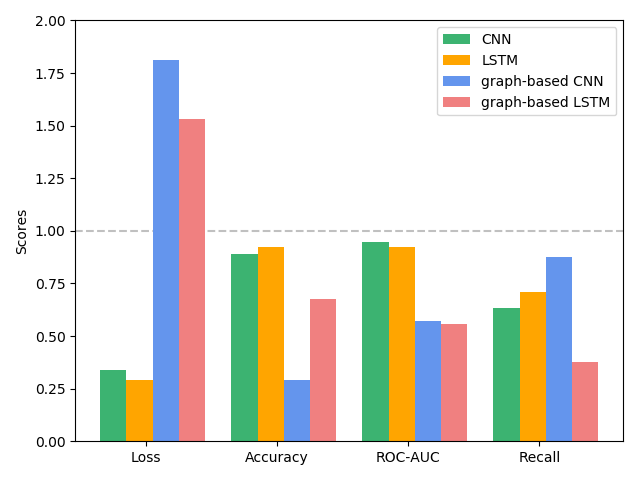
\includegraphics[width=0.7\textwidth]{pred_sequence500_plots}
    \caption{Barplot of results of the models for the problem of prediction on a sequence with the target 500 time steps (1 second) forward}
    \label{fig:pred_sequence500_plots}
\end{figure}

For this configuration, the CNN model looked at sequences of 500 time steps each; the LSTM model looked at sequences of 200 time steps each; both the graph-based models looked at sequences of 5000 time steps each, corresponding to 10 graphs, each one representing a window of 500 time steps.

Table \ref{tab:pred_sequence1000_results} and the barplot in Figure \ref{fig:pred_sequence1000_plots} show the results for the prediction of a target 1000 time steps (2 seconds) forward with respect to the associated sequence.
\begin{table}[htbp]
    \centering
    \begin{tabular}{lllll}
        \hline
                          & \multicolumn{4}{c}{\textbf{Metric}}                                    \\ \cline{2-5} 
        \textbf{Model}    & \textit{loss} & \textit{accuracy} & \textit{ROC-AUC} & \textit{recall} \\ \hline
        CNN               & 0.224         & 92.4 \%           & 0.930            & \textbf{0.702}  \\
        LSTM              & 0.180         & 95.4 \%           & 0.908            & 0.637           \\
        graph-based CNN   & 2.990         & 32.9 \%           & 0.661            & 0.779           \\
        graph-based LSTM  & 1.524         & 61.4 \%           & 0.547            & 0.439           \\\hline
    \end{tabular}
    \caption{Results of the models for the problem of prediction on a sequence with the target 1000 time steps (2 seconds) forward}
    \label{tab:pred_sequence1000_results}
\end{table}

\begin{figure}[htbp]
    \centering
    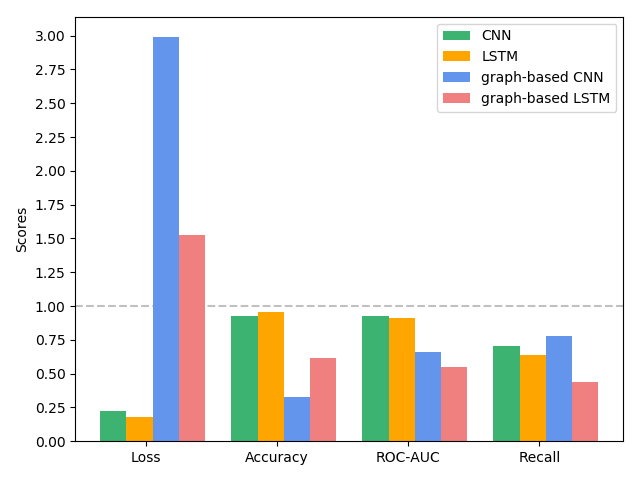
\includegraphics[width=0.7\textwidth]{pred_sequence1000_plots}
    \caption{Barplot of results of the models for the problem of prediction on a sequence with the target 1000 time steps (2 seconds) forward}
    \label{fig:pred_sequence1000_plots}
\end{figure}

For this configuration, the CNN model looked at sequences of 200 time steps each; the LSTM model looked at sequences of 500 time steps each; both the graph-based models looked at sequences of 5000 time steps each, corresponding to 10 graphs, each one representing a window of 500 time steps.

Table \ref{tab:pred_sequence2000_results} and the barplot in Figure \ref{fig:pred_sequence2000_plots} show the results for the prediction of a target 2000 time steps (4 seconds) forward with respect to the associated sequence.
\newpage
\begin{table}[htbp]
    \centering
    \begin{tabular}{lllll}
        \hline
                          & \multicolumn{4}{c}{\textbf{Metric}}                                    \\ \cline{2-5} 
        \textbf{Model}    & \textit{loss} & \textit{accuracy} & \textit{ROC-AUC} & \textit{recall} \\ \hline
        CNN               & 0.236         & 94.0 \%           & 0.911            & 0.604           \\
        LSTM              & 0.204         & 95.6 \%           & 0.932            & \textbf{0.767}  \\
        graph-based CNN   & 2.549         & 32.8 \%           & 0.642            & 0.790           \\
        graph-based LSTM  & 2.103         & 46.7 \%           & 0.475            & 0.463           \\\hline
    \end{tabular}
    \caption{Results of the models for the problem of prediction on a sequence with the target 2000 time steps (4 seconds) forward}
    \label{tab:pred_sequence2000_results}
\end{table}

\begin{figure}[htbp]
    \centering
    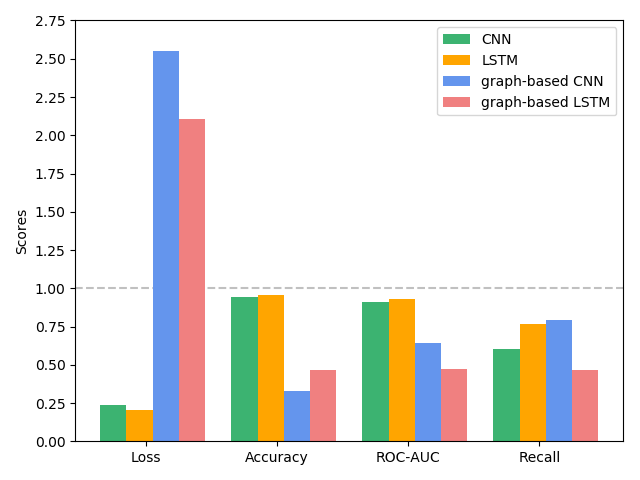
\includegraphics[width=0.7\textwidth]{pred_sequence2000_plots}
    \caption{Barplot of results of the models for the problem of prediction on a sequence with the target 2000 time steps (4 seconds) forward}
    \label{fig:pred_sequence2000_plots}
\end{figure}

For this configuration, the CNN model looked at sequences of 500 time steps each; the LSTM model looked at sequences of 500 time steps each; both the graph-based models looked at sequences of 5000 time steps each, corresponding to 10 graphs, each one representing a window of 500 time steps.

\paragraph{} As regards to the first case (\texttt{'target steps ahead'}=500) and the third case (\texttt{'target steps ahead'}=2000), the \acs{lstm} model obtained the best results, while in the second case (\texttt{'target steps ahead'}=1000) the \acs{cnn} performed better. In general, the two models were able to achieve about 0.70 of recall, which is a great result considering the extremely limited amount of data. The \acs{lstm} obtained the absolute best result with a recall equal to 0.767 for the prediction on a sequence with the target 4 seconds forward.

On the other hand, the performances of the graph-based models were unsatisfactory and very similar to the ones obtained on the task of detection on a sequence. Also in this case, the high recall reached by the graph-based \acs{cnn} is due to a prediction that is almost random, as suggested by the ROC-AUC values, and that most of the time is equal to 1, leading to a low accuracy and very high loss.


\subsection{Comments on the results}
\paragraph{} In general, the results obtained from the experiments were very respectable, given the complexity of the problem and the restricted amount of data. Based on the results, we were able to confirm some assumption, but also to reconsider other ideas.

The task of seizure detection based on a single time step confirmed our expectations: probably the information to correctly detect a seizure is partially included in the time series and not expressed only by the features of a single time step. This is confirmed also by the fact that the models obtained good results on the same task of detection, but based on a sequence. Surprisingly, the task on which the models performed better was the most difficult one, that is the seizure prediction based on a sequence. For this task, the models where able to achieve a recall higher than 0.70, which is an excellent result considering the few data used compared to previous approaches, where way more data have been used.

Overall, the model that performed better was the \acs{lstm} neural network, which most of the times obtained the highest value for recall, accuracy and ROC-AUC and the lowest value for the loss. Also the \acs{cnn} model performed very well, obtaining similar results. The models that curiously did not obtain the results expected were the graph-based \acs{cnn} and \acs{lstm} models. We tested these models with the assumption that they could outperform the standard deep learning models, since the graph representation of the brain activity is a common practice in the field of neuroscience and the application of graph-based models has recently produced good results. Unfortunately, the performances achieved by the graph-based models in this project were really poor, as we were not able to identify a good threshold between overfitting and underfitting.

There could be several reasons explaining the poor performances of the graph-based models on this type of tasks. First of all, these models were trained on graphs representing the functional connectivity between electrodes and functional connectivity networks are extremely sensitive to the choice of the connectivity metric, which in our case was the correlation coefficient. It is possible that the information that characterize the epileptic phenomenon did not arise from the configuration used to create the graphs, even if the connectivity metric has been chosen based on the literature. Another reason for the poor results obtained is the fact that graph-based models significantly suffer the lack of data. This could be a big problem for the seizure prediction task, since in a real-world scenario, seizure data are difficult to gather and we tried to reproduce a setting as real as possible by limiting the amount of available data. Therefore, this could explain why our graph-based models obtained bad performances in comparison to other studies about graph-based epileptic seizure detection which use datasets containing up to thousands of seizures (i.e. \cite{arXiv:graphseizuredet}).
\clearpage
%************************************************
% CONCLUSION
%************************************************

\chapter{Conclusion} \label{chap: conclusion}

\paragraph{} In this work, we provided an overview of machine learning and deep learning methods applied to the task of seizure prediction.

We started by acquiring knowledge about the seizure prediction task and defining three different settings, namely detection on a single time step, detection on a sequence and prediction on a sequence. We worked with a limited amount of data in order to replicate a real-world scenario, where seizures data are highly difficult to gather. In order to test the models on the seizure prediction task, we ran several experiments for the various combinations of models and problem cases, looking for the models configurations that achieved the best performances. We made a comparison between the results of different models across the three problem cases and to identify the methods that worked better on each task. Thanks to the experiments, we were able to confirm of reject some assumptions we made at the beginning and to create new hypotheses based on the results.

By running several experiments and fine-tuning the models hyperparameters, we were able to predict a seizure up to 4 seconds in the future, achieving a recall of 0.767 on the test set, matched by high values for accuracy and ROC-AUC and a low loss. The model that was able to obtain these excellent performances is an \acs{lstm} neural network, which was also the best performer overall. The obtained results are noteworthy considering that the models has been trained and tested on a dataset containing only three seizures, representing an extremely challenging set-up for a such complex problem.

Our project demonstrated the ability of deep learning models to achieve good results on the seizure prediction task even in a situation characterized by a significant lack of data. It also showed that graph deep learning models, on the other hand, are not able to handle this extreme case scenario with the configuration proposed.

Future works on this project could involve a research on a bigger scale, testing a higher amount of machine learning and deep learning models and using some additional data preprocessing technique to improve performances, while still keeping the dataset fairly small to be more realistic. Another interesting deepening could be a study about how to create functional connectivity networks for this type of task, testing different connectivity metrics in order to identify the ones that improve performances. \clearpage
%************************************************
% RANDOM STUFF
%************************************************

\chapter*{Notes}
\addcontentsline{toc}{chapter}{Notes}
\chaptermark{Notes}
% \minitoc

\paragraph{Topics}
\begin{itemize}
    \item Intro (big summary of the thesis)
    \subitem Problem statement
    \subitem What (GNN, LSTM, etc.)
    \item Background (theoretical explanation of models used and SOTA)
    \subitem Machine learning methods
    \subitem Neural Networks
    \subitem Dense
    \subitem LSTM
    \subitem Conv
    \subitem GNN
    \subitem Seizure prediction
    \subitem EEG
    \subitem Functional connectivity network
    \subitem State of the art
    \item Methods (description of all the work done and motivations, but no numbers)
    \subitem Baseline
    \subitem Graph / contribution
    \item Experiments/Implementation (technical description of all the work done with parameters and numbers)
    \subitem Environment (software, server, framework)
    \subitem Data + preprocessing
    \subitem Architectures (params)
    \subitem Results
    \item Conclusions
    \subitem Comments
    \subitem Future work
\end{itemize}

\paragraph{Project steps}
\begin{itemize}
    \item Baseline
    \subitem Detection
    \subitem --- Random Forest
    \subitem --- Gradient Boosting
    \subitem --- SVM
    \subitem --- Dense
    \subitem --- LSTM
    \subitem --- Convolution
    \subitem Prediction
    \subitem --- LSTM
    \subitem --- Convolution
    \subitem ------ Stride > 1 and bigger look\_back
    \subitem ------ Parameters search
    \item Graph Neural Networks
    \subitem GNN + LSTM
    \subitem GNN + Conv1D
    \subitem \textbf{TODO} Pooling
    \subitem --- \textbf{TODO} Hierarchical (Rex Ying)
    \subitem --- \textbf{TODO} Decimation (Bianchi)
    \item Baseline
    \subitem \textbf{TODO} Cross Validation on 3 seizures
    \subitem \textbf{TODO} Bayesian optimization
    \subitem \textbf{TODO} Different functional connectivity nets
    \subitem \textbf{TODO} Big data
    \subitem \textbf{TODO} Structural connectivity (KNN)
\end{itemize}

\todo[inline]{
    Missing experiments: Detection with graph-based models, cross-validation on detection tasks
}


\section{General considerations}

\subsection{IEEG plots}
\paragraph{} The ieeg plots give an overall idea of the type of data to deal with and of the shape of the patient's seizures. On 24 hours of recording, there are three seizures in the first 3 hours. The data is divided in clips of 1 hour each, containing 1800000 timestamps each (the signal is sampled at 500Hz). The three seizures found have a duration between 13000 and 15000 timestamps each (between 26 and 30 seconds).

The ieeg doesn't explicitly show the presence of a seizure; indeed the dynamic of the electrodes signals doesn't change in correspondence of the beginning of a seizure. For example, in the first seizure the signals dynamic remains pretty stable during the first half of the seizure and suddenly changes at the beginning of the second half of the seizure. This behaviour suggests that the seizure is not directly represented by the dynamic of the signals, but it is represented by the non-linear relations between the electrodes behaviours.

The ieeg plots show an interesting thing: in all the three seizures, there are two electrodes that are more dynamic exactly during the seizure. In the plots they are always represented with green colour.
\begin{itemize}
    \item classic plot (with y values): electrodes signals positioned at -5000 and 2500.
    \item norm plot (y normalised): electrodes signals positioned at 8th position from the top and 33th position from the bottom.
\end{itemize}


\section{Machine learning classic models}

\subsection{Experiments with classic methods}
\paragraph{} The three machine learning classic methods used to perform experiments are random forest, gradient boosting and support vector machine. All the three methods have been implemented using scikit learns modules; for gradient boosting also xgboost library has been used. For all the experiment just portions containing seizures of the entire dataset have been used to train and to test data in order to speed up the process and to reduce the huge difference of availability of data between the two classes.

Classic methods have been used only for the detection task, since they are not powerful enough in order to deal with the prediction task, at least with this kind of data.

\paragraph{Parameters:}
\begin{itemize}
    \item random forest:
        \subitem number of estimators: 100
        \subitem maximum depth: 10
        \subitem both balanced and non-balanced class weight
    \item gradient boosting:
        \subitem number of estimators: 100
        \subitem maximum depth: 10
    \item svm:
        \subitem gamma: scale
        \subitem both weighted and non-weighted classes
\end{itemize}

In all the experiments, seizure 2 and 3 have been used as training set, while seizure 1 has been used as test set.
\todo[inline]{Maybe try to cross-validate by exchanging datasets for training and testing.}

\paragraph{Results:} All the experiments had almost the same results:
\begin{itemize}
    \item Loss: around 0.15
    \item Accuracy: around 0.85
    \item Roc auc: around 0.65
\end{itemize}

Only the unbalanced random forest was able to get almost decent results:
\begin{itemize}
    \item Loss: 0.11
    \item Accuracy: 0.85
    \item Roc auc: 0.73
\end{itemize}

The results are very bad and show that the classic methods are too weak to be able to solve this problem having to deal with such a complex and unbalanced dataset. Indeed, the area under the Roc curve is around 0.65 for the majority of the models, which means that the predictions are made almost in a random way.
\todo[inline]{Maybe try using some different metric (ex. F1)}

The predictions have also been plotted in order to have a better idea of what was predicted wrong and where and also the plots show a non-logical distribution, even if in some cases (for example in the non-balanced experiment with the random forest) the predictions in the seizure area seem to match with the targets. Also in the gradient boosting experiment, the model seems to start predicting 1 (there is a seizure) in the same timestamps in which the signals in the ieeg start to be more dynamic (almost in the middle of the seizure 1).


\section{Deep learning classic models}

\subsection{Dense neural network}

A dense neural network have been built in order to deal with the seizure detection task. After some hyperparameters tuning, the final structure of the network was the following:

\paragraph{Parameters:} These are the parameters used in the network's layers.
\begin{itemize}
    \item[-] activation: tanh
    \item[-] kernel regularisation: L2(5e-4)
    \item[-] class weight: \{0: len(y\_train) / n\_negative, len(y\_train / n\_positive\}
\end{itemize}

\paragraph{Structure:} These are the layers used to build the network.
\begin{lstlisting}
Dense(units: 512)
Dropout(0.5)
Dense(units: 512)
Dropout(0.5)
Dense(units: 256)
Dropout(0.5)
Dense(units: 1, activation: 'sigmoid')
\end{lstlisting}

In order to compile the model, binary cross-entropy has been used as loss and Adam as optimiser.

Initially the structure was composed by less layers and each one with less units (ex. 128, 156), but the model wasn't powerful enough so both the number of layers and units have been increased. The kernel regularisation and the dropout layers have been added in order to avoid overfitting on training data. For the activation of the dense layers, both tanh and ReLu have been tried, but for some reason tanh works way better. Since the two classes of the problem, that are "seizure" (1) and "not-seizure" (0), are very unbalanced due to the small presence of seizure timestamps with respect to the number of non-seizure timestamps, class weight has been used to train the network. The weight assigned to each class is inversely proportional to the number of timestamps of that class with respect to the total number of timestamps.

Initially, in order to preprocess the data, the MinMaxScaler from scikit-learn library was used, but then it was substituted by the StandardScaler because this one led to better performances. The data are also shuffled in order to help the network to generalise.

Initially, as for the machine learning classic methods, just portions containing seizures of the entire dataset have been used to train and to test data. In order to do some test, a modification of the initial dataset has been tried: the dataset has been modified so that each clip is trimmed ending with the end of the seizure and starting 100,000 timestamps before the end of the seizure. The intention of this test was to eliminate the useless bias generated by the timestamps after the seizure. However, after testing it, for some reason the results got a lot worse, so the old portions of the dataset have been used for the next experiments.

\paragraph{Results} After all the tuning described above, the best results that the dense network got on the detection task were the following:
\begin{itemize}
    \item Loss: 0.87
    \item Accuracy: 0.79
    \item Roc auc: 0.74
\end{itemize}

These results are not extremely good but they are ok considering the complexity of the problem. The dense network behaved in a similar way to the unbalanced random forest, looking at the results. Looking at the plots of the predictions, they don't seem to be very promising, but in order to better understand the behaviour of the prediction, also the running mean have been plotted and it explicitly shows that the network is able to understand where is the seizure.

A strange thing happens in the predictions: in the test prediction plot, there is a sort of a "hole" of zero predictions right after the end of the seizure.

\subsection{LSTM neural network}

\paragraph{} I built an LSTM network in order to deal both with the detection and the prediction tasks.

For this network, I introduced subsampling to the data preprocessing. The subsampling function take as input the subsampling factor, which represent how many negative examples we want to keep with respect to the positive ones. In this way, we can consistently reduce the disparity in the amount of positive and negative examples, preserving all the positive ones. The subsampling was performed both for the detection and the prediction task. The subsampling factor was set to 2, so that for each positive samples there are two negative ones. The stride in the subsampling was set to 1 in order to keep all the (positive) samples.

Another function was used in order to generate the sequences of data and labels to give as input to the network. It takes the parameters "look\_back", which is the length of the input sequence (how many samples do I look behind), and "target\_steps\_ahead", which represents how many steps ahead to predict (how many samples there are between the end of the input sequence and the future sample I want to predict). Given this two parameters, it creates the pairs input\_sequence - target accordingly.

For the detection task, the parameter "target\_steps\_ahead" was set to 0, that is the target corresponding to the last sample of the input sequence. For the prediction task, obviously the parameter was set to some values higher than 0, as we want to predict the target of a sample in the future, that wasn't inside the input sequence.

\paragraph{Detection task} For the detection task, after some hyperparameter search and tuning, the best result was given by these parameters (experiment 147):
\begin{lstlisting}
epochs:			10
batch_size:		64
depth_lstm:		1
depth_dense:	2
units_lstm:		256
reg:            l2(5e-1)
activation:		relu
batch_norm:		True
dropout:        0.4
class_weight:	{0: 0.4682, 1: 3.0}
look_back:		100
stride:			1
predicted_timestamps:	1
target_steps_ahead:		0
subsampling_factor:		2
\end{lstlisting}

The network was build in this way:

\begin{lstlisting}
LSTM(units: 256)
BatchNormalization()
Dropout(0.4)
Dense(units: 256)
BatchNormalization()
Dropout(0.4)
Dense(units: 1, activation: 'sigmoid')
\end{lstlisting}

The results on an input sequence of length 100 were:

\begin{itemize}
    \item Loss: 0.2632
    \item Accuracy: 0.9059
    \item Roc auc: 0.9263
\end{itemize}

\paragraph{Prediction task} For the prediction task, after some hyperparameter search and tuning, the best result was given by these parameters (experiment 20):
\begin{lstlisting}
epochs:			10
batch_size:		64
depth_lstm:		1
depth_dense:	2
units_lstm:		256
reg:            l2(5e-1)
activation:		relu
batch_norm:		True
dropout:        0.4
class_weight:	{0: 1.1561, 1: 7.4074}
look_back:		200
stride:			1
predicted_timestamps:	1
target_steps_ahead:		2000
subsampling_factor:		2
\end{lstlisting}

The network was build in this way:

\begin{lstlisting}
LSTM(units: 256)
BatchNormalization()
Dropout(0.4)
Dense(units: 256)
BatchNormalization()
Dropout(0.4)
Dense(units: 1, activation: 'sigmoid')
\end{lstlisting}

The results on an input sequence of length 100 and a target steps ahead of 2000 were:

\begin{itemize}
    \item Loss: 0.3098
    \item Accuracy: 0.9454
    \item Roc auc: 0.9337
\end{itemize}

The network that performed better was the same for both the detection and prediction tasks, even with the same regularisation parameters. What changed was, of course, the distance of the sample predicted and the length of the input sequence. The LSTM, in both the situation, wasn't able to deal with more than 200 samples in the input sequence (the results were way worse with a higher value). For the prediction task, the network was able to successfully predict until 2000 steps ahead, which correspond to 4 seconds. Higher than that, the prediction became almost random.


\subsection{Convolutional neural network}

\paragraph{} I built a CNN in order to deal both with the detection and the prediction tasks.

For this network, as for the LSTM, I introduced subsampling to the data preprocessing (see LSTM).The subsampling was performed both for the detection and the prediction task. The subsampling factor was set to 2, so that for each positive samples there are two negative ones. Another function was used in order to generate the sequences of data and labels to give as input to the network (see LSTM).

\paragraph{Detection task} For the detection task, we used the same parameter we found for the LSTM, except for the look\_back, that in the case of the convolutional can be much higher. The best result was given by these parameters (experiment 2):
\begin{lstlisting}
epochs:			10
batch_size:		64
depth_conv:		5
depth_dense:	2
filters:        512
kernel_size:	5
reg:            l2(5e-1)
activation:		relu
batch_norm:		True
dropout:        0.4
class_weight:	{0: 1.1561, 1: 7.4074}
look_back:		1000
stride:			1
predicted_timestamps:	1
target_steps_ahead:		0
subsampling_factor:		2
\end{lstlisting}

\todo[inline]{Run again experiments for detection with CNN using less filters and smaller kernel size}

The network was build in this way:

\begin{lstlisting}
Conv1D(filters: 512)
MaxPooling1D()
Conv1D(filters: 512)
MaxPooling1D()
Conv1D(filters: 512)
MaxPooling1D()
Conv1D(filters: 512)
MaxPooling1D()
Conv1D(filters: 512)
MaxPooling1D()
Flatten()
Dense(units: 256)
BatchNormalization()
Dropout(0.4)
Dense(units: 1, activation: 'sigmoid')
\end{lstlisting}

The results on an input sequence of length 1000 were:

\begin{itemize}
    \item Loss: 0.1550
    \item Accuracy: 0.9374
    \item Roc auc: 0.9870
\end{itemize}

\paragraph{Prediction task} For the prediction task, I began with some hyperparameter search and tuning using the same parameters used for the LSTM as initial model. The best result was given by these parameters (experiment 29):
\begin{lstlisting}
epochs:			10
batch_size:		64
depth_conv:		5
depth_dense:	2
filters:        256
kernel_size:	5
reg:            l2(5e-1)
activation:		relu
batch_norm:		True
dropout:        0.4
class_weight:	{0: 1.1560, 1: 7.4074}
look_back:		1000
stride:			1
predicted_timestamps:	1
target_steps_ahead:		2000
subsampling_factor:		2
\end{lstlisting}

The network was build in this way:

\begin{lstlisting}
Conv1D(filters: 256)
MaxPooling1D()
Conv1D(filters: 256)
MaxPooling1D()
Conv1D(filters: 256)
MaxPooling1D()
Conv1D(filters: 256)
MaxPooling1D()
Conv1D(filters: 128)
MaxPooling1D()
Flatten()
Dense(units: 256)
BatchNormalization()
Dropout(0.4)
Dense(units: 1, activation: 'sigmoid')
\end{lstlisting}

The results on an input sequence of length 100 and a target steps ahead of 2000 were:

\begin{itemize}
    \item Loss: 0.2598
    \item Accuracy: 0.9314
    \item Roc auc: 0.9274
\end{itemize}

For the prediction task, the network was able to successfully predict until 2000 steps ahead, which correspond to 4 seconds. Higher than that, the prediction became almost random.


\todo[inline]{CNN notes}


\clearpage
% %************************************************
% APPENDIX
%************************************************

\appendix %optional, use only if you have an appendix

\chapter{Some retarded material}
\section{It's over\dots}
\lipsum \clearpage


%************************************************
% FINAL SECTION
%************************************************
\backmatter

% \nocite{*}
\bibliographystyle{unsrtnat} %plainnat
\bibliography{corpus/biblio}
%\chapter{Glossary} %optional
% \input{corpus/bibliography}\clearpage


%\cleardoublepage
%\theindex %optional, use only if you have an index, must use
%\makeindex in the preamble

\end{document}



% BIBLIOGRAPY STUFF as example

% @article{einstein,
%     author =       "Albert Einstein",
%     title =        "{Zur Elektrodynamik bewegter K{\"o}rper}. ({German})
%         [{On} the electrodynamics of moving bodies]",
%     journal =      "Annalen der Physik",
%     volume =       "322",
%     number =       "10",
%     pages =        "891--921",
%     year =         "1905",
%     DOI =          "http://dx.doi.org/10.1002/andp.19053221004"
% }
 
% @book{latexcompanion,
%     author    = "Michel Goossens and Frank Mittelbach and Alexander Samarin",
%     title     = "The \LaTeX\ Companion",
%     year      = "1993",
%     publisher = "Addison-Wesley",
%     address   = "Reading, Massachusetts"
% }
 
% @misc{knuthwebsite,
%     author    = "Donald Knuth",
%     title     = "Knuth: Computers and Typesetting",
%     url       = "http://www-cs-faculty.stanford.edu/\~{}uno/abcde.html"
% }